%%%%%%%%%%%%%%%%%%%%%%%%%%%%%%%%%%%%%%%%%%%%%%%%%%%%%%%%%%%%%

%%%%%%%%%%%%%%%%%%%%%%%%%%%%%%%%%%%%%%%%%%%%%%%%%%%%%%%%%%%%%
%% HEADER
%%%%%%%%%%%%%%%%%%%%%%%%%%%%%%%%%%%%%%%%%%%%%%%%%%%%%%%%%%%%%
\documentclass[letterpaper,twoside,12pt]{report}
% Alternative Options:
%	Paper Size: a4paper / a5paper / b5paper / letterpaper / legalpaper / executivepaper
% Duplex: oneside / twoside
% Base Font Size: 10pt / 11pt / 12pt

%% Language %%%%%%%%%%%%%%%%%%%%%%%%%%%%%%%%%%%%%%%%%%%%%%%%%
\usepackage[spanish]{babel} %francais, polish, spanish, ...
\usepackage[T1]{fontenc}
%\usepackage[ansinew]{inputenc}
%\usepackage[latin1]{inputenc}
\usepackage[utf8]{inputenc}
\usepackage{enumitem}

\usepackage{lmodern} %Type1-font for non-english texts and characters

%% Packages for Graphics & Figures %%%%%%%%%%%%%%%%%%%%%%%%%%
\usepackage{graphicx} %%For loading graphic files
\usepackage{float} %%For loading graphic files

%% Math Packages %%%%%%%%%%%%%%%%%%%%%%%%%%%%%%%%%%%%%%%%%%%%
%\usepackage{amsmath}
\usepackage{amsthm}
\usepackage{amssymb, amsmath} %Paquetes matemáticos de la American Mathematical Society
\usepackage{amsfonts}

\usepackage{multirow} %for tables
\usepackage{booktabs}  % Líneas horizontales de calidad

%% Line Spacing %%%%%%%%%%%%%%%%%%%%%%%%%%%%%%%%%%%%%%%%%%%%%
%\usepackage{setspace}
%\singlespacing        %% 1-spacing (default)
%\onehalfspacing       %% 1,5-spacing
%\doublespacing        %% 2-spacing

%% Other Packages %%%%%%%%%%%%%%%%%%%%%%%%%%%%%%%%%%%%%%%%%%%
\usepackage{parskip}
\usepackage{tabularx}
\usepackage{array, ragged2e}
%\usepackage{fancyhdr} %%Fancy headings
%\usepackage{longtable} %%For tables, that exceed one page
%\usepackage{quthesis}%

\hyphenation{com-por-ta-mien-to in-ter-pre-ta-ci\'on con-di-cio-nes mo-vi-mien-tos}

\makeatletter
 \def\@textbottom{\vskip \z@ \@plus 1pt}
 \let\@texttop\relax
\makeatother

%%%%%%%%%%%%%%%%%%%%%%%%%%%%%%%%%%%%%%%%%%%%%%%%%%%%%%%%%%%%%
%% DOCUMENT
%%%%%%%%%%%%%%%%%%%%%%%%%%%%%%%%%%%%%%%%%%%%%%%%%%%%%%%%%%%%%

\begin{document}
\title{Apuntes y Conceptualizaciones aprendidos durante el curso Pollitos Sept-Oct/2024}
\author{by\\Daniel Orozco
\\
\\
\\
\\Esta es una serie de apuntes y notas
\\que he podido tomar y seguir consultando
\\luego de haber participado en el curso Sept-Oct/2024
\\con el lobo alfa de Precio y Volumen
\\
\\
\\
\\Santiago de Cali, Valle del Cauca, Colombia
}
\date{Marzo 2025}
\maketitle

\chapter*{Resumen}

Lo que aqu\'i expongo lo hago a t\'itulo personal y es cada uno de los conceptos que voy aprendiendo a reconocer en vivo y a diario.

No es de extra\~{n}ar que, mientras perfecciono, se presenten errores de conceptualizaci\'on.

Sin embargo, dispuesto estoy a corregir y a aprender correctamente. Pues de esto se trata esta actividad, de un constante aprendizaje y repaso de lo ya aprendido.

\chapter*{Agradecimientos}

Inicialmente a mi mentor, el lobo alfa, a qui\'en quiero parecerme, (aclaro), en su estilo de operativa y nivel de acierto. 

A mi esposa que ha sufrido conmigo este cambio de actividad y dice que cree en m\'i, y yo le creo.

\newpage
\tableofcontents
\chapter{Introducci\'on}

Paso a paso ir\'e construyendo este apartado hasta que considere que est\'a muy bien escrito y que realmente puede orientar a un futuro lector. Inicialmente este escrito es s\'olo para m\'i.

%\section{Results}

\section{Aportes y Contribuciones}
Ya lo dije anteriormente, en la medida que pueda ir aportando conocimiento lo har\'e:
\begin{itemize}
	\item Mostrar los conceptos.
	\item Establecer mi sistema.
	\item Mostrar mi operativa.
\end{itemize}

\section{Descripci\'on}
Indicar c\'omo est\'a esteblecido el presente documento.
Chapter 3 muestra...

Chapter 4 describe ....

Chapter 5 conclusiones y aportes...
\chapter{Conceptos}

\section{Conceptos Clave en la Lectura Profesional}

\subsection{Intenci\'on}

La \textbf{intenci\'on} se define como el prop\'osito oculto del operador profesional para influir en la direcci\'on del precio, manifest\'andose mediante patrones en volumen y velas. Se evidencia al observar:

\begin{itemize}
    \item Entrada relevante de volumen.
    \item Movimientos verticales y r\'apidos.
    \item Ruptura de zonas relevantes como rangos, soportes o resistencias y claviculares.
\end{itemize}

\begin{figure}[htb]
    \centering
    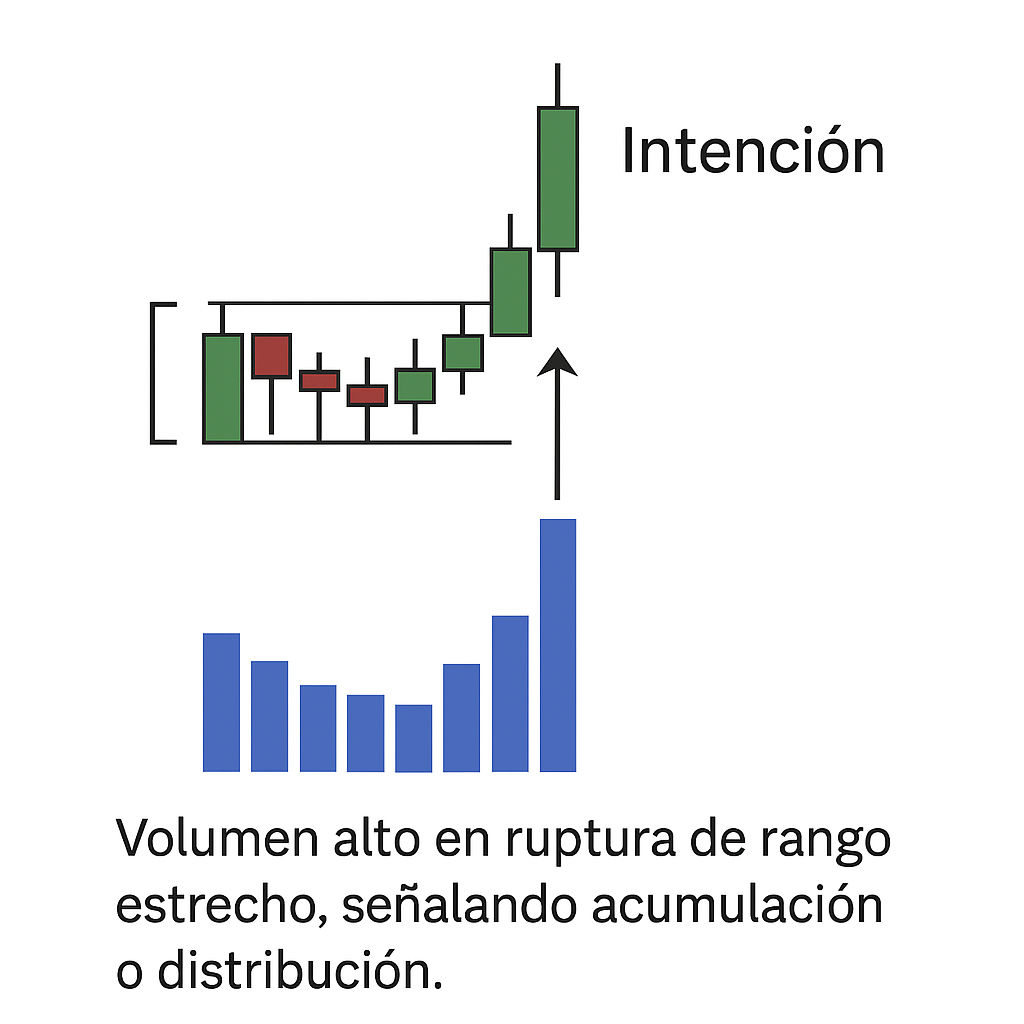
\includegraphics[width=11cm]{images/Intencion.png}
    \caption{Intenci\'on}
    \label{fig:Intencion}
\end{figure}

En la figura \ref{fig:Intencion} ...

\subsection{Desequilibrio}

El \textbf{desequilibrio} ocurre cuando una fuerza (oferta o demanda) domina claramente, impulsando movimientos significativos:

\begin{itemize}
    \item Se evidencia en velas amplias con alto volumen.
    \item Genera fases impulsivas como markup o markdown.
\end{itemize}

La combinaci\'on de estos elementos (intenci\'on, testeo y secado) facilita identificar momentos ideales para actuar en direcci\'on al desequilibrio.

\vspace{1em}
\noindent

\begin{figure}[!htbp]
    \centering
    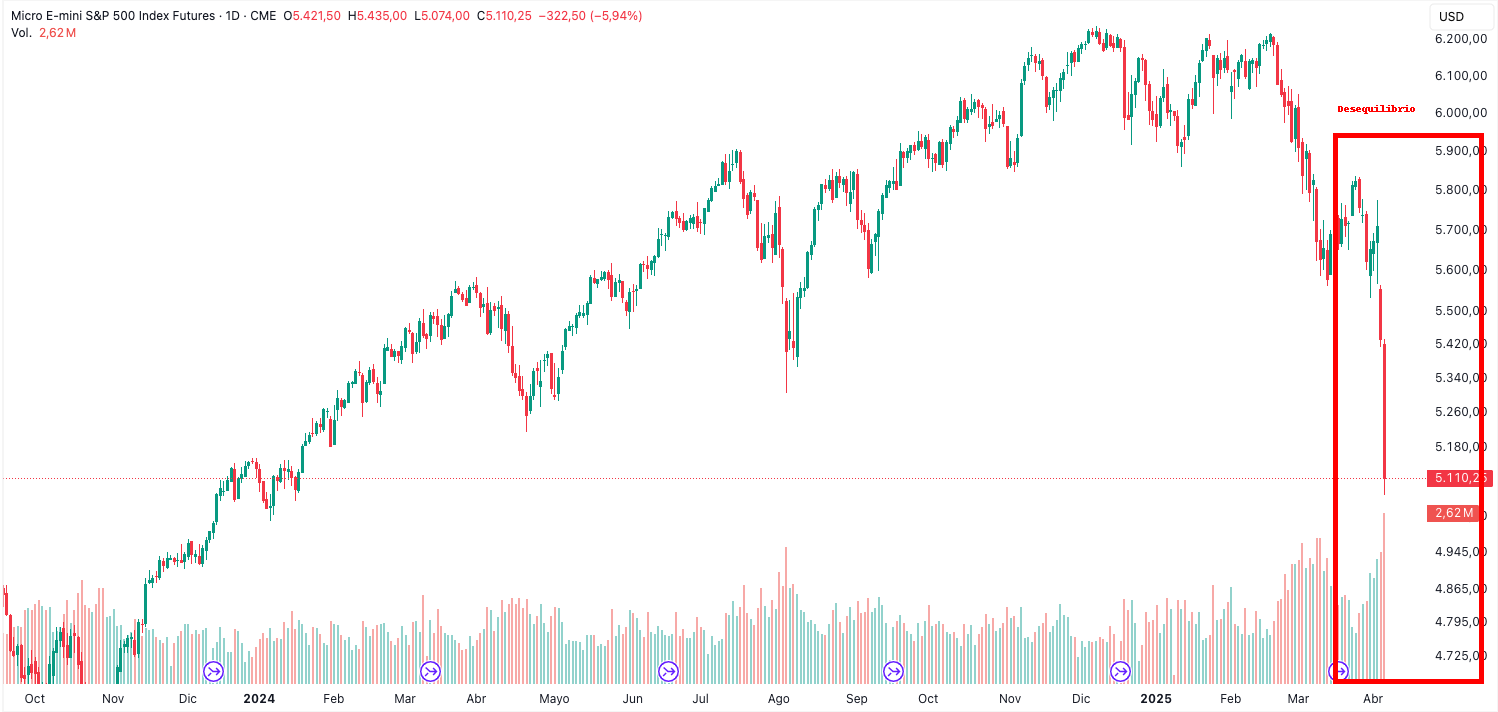
\includegraphics[width=11cm]{images/desequilibrio_mes0625_ampliado.png}
    \caption{Desequilibrio}
    \label{fig:desequilibrio_mes0625_ampliado}
\end{figure}
\vspace{0.5em}
\noindent

\subsection{Ejemplo de Desequilibrio en el MES-0625 (Abril 2025)}

En el contrato \textbf{MES-0625}, en el marco diario correspondiente al 4 de abril de 2025, figura \ref{fig:desequilibrio_mes0625_ampliado}, se observa un claro ejemplo de \textbf{desequilibrio bajista}:

\begin{itemize}
    \item El precio presenta una \textbf{vela bajista de cuerpo amplio}, con un rango significativamente mayor al promedio reciente.
    \item Esta vela rompe m\'ultiples soportes anteriores, generando una fase impulsiva tipo \textit{markdown}.
    \item El volumen asociado es el m\'as alto del per\'iodo observado, alcanzando los \textbf{2{,}62 millones de contratos}, lo cual confirma \textbf{intenci\'on profesional} en la acci\'on vendedora.
\end{itemize}

La combinaci\'on de una vela de amplio rango con volumen extremo constituye una manifestaci\'on clara de desequilibrio, validando la dominancia de la oferta en ese tramo del mercado.


\subsection{Secado}

El \textbf{secado} refleja la retirada deliberada de una de las partes profesionales del mercado:

\begin{itemize}
    \item Se caracteriza por un volumen muy bajo posterior a un movimiento.
    \item Suele preceder o formar parte del testeo.
    \item Indica ausencia de presi\'on contraria.
\end{itemize}

\begin{figure}[!htbp]
    \centering
    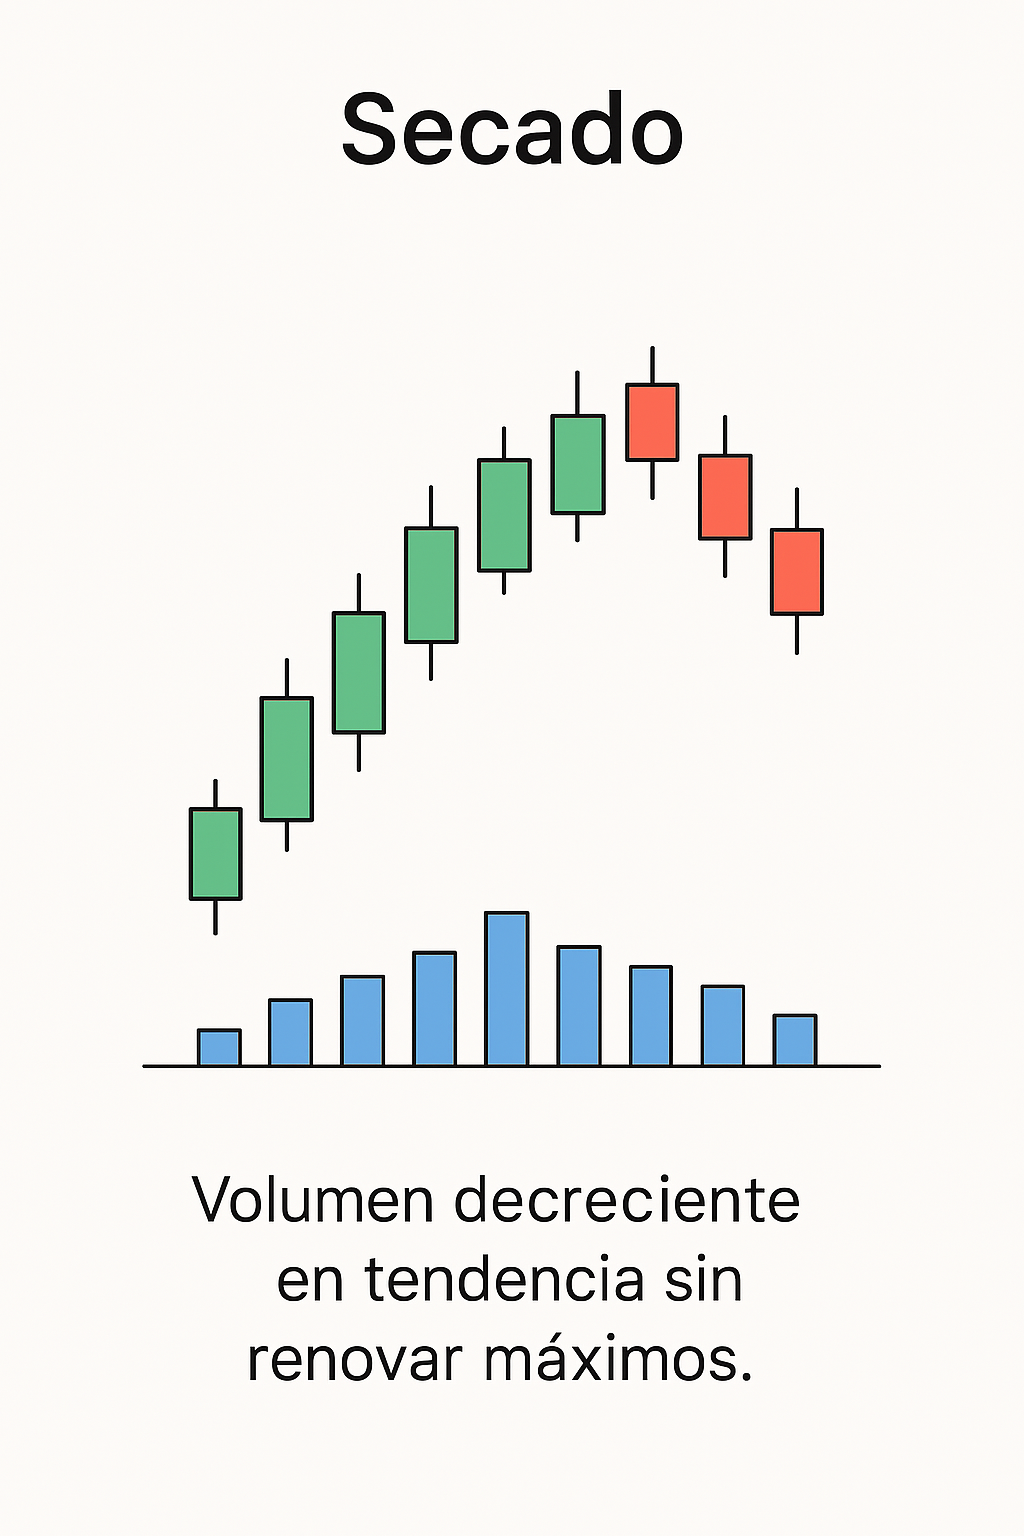
\includegraphics[width=11cm]{images/Secado.png}
    \caption{Secado}
    \label{fig:Secado}
\end{figure}

En la figura \ref{fig:Secado} ...

\subsection{Testeo}

El \textbf{testeo} es un movimiento correctivo con volumen estable o decreciente para evaluar si persiste presi\'on contraria tras una intenci\'on manifiesta:

\begin{itemize}
    \item No debe superar el origen del movimiento intencional previo.
    \item Si ocurre, debe recuperarse r\'apidamente.
\end{itemize}

\begin{figure}[!htbp]
    \centering
    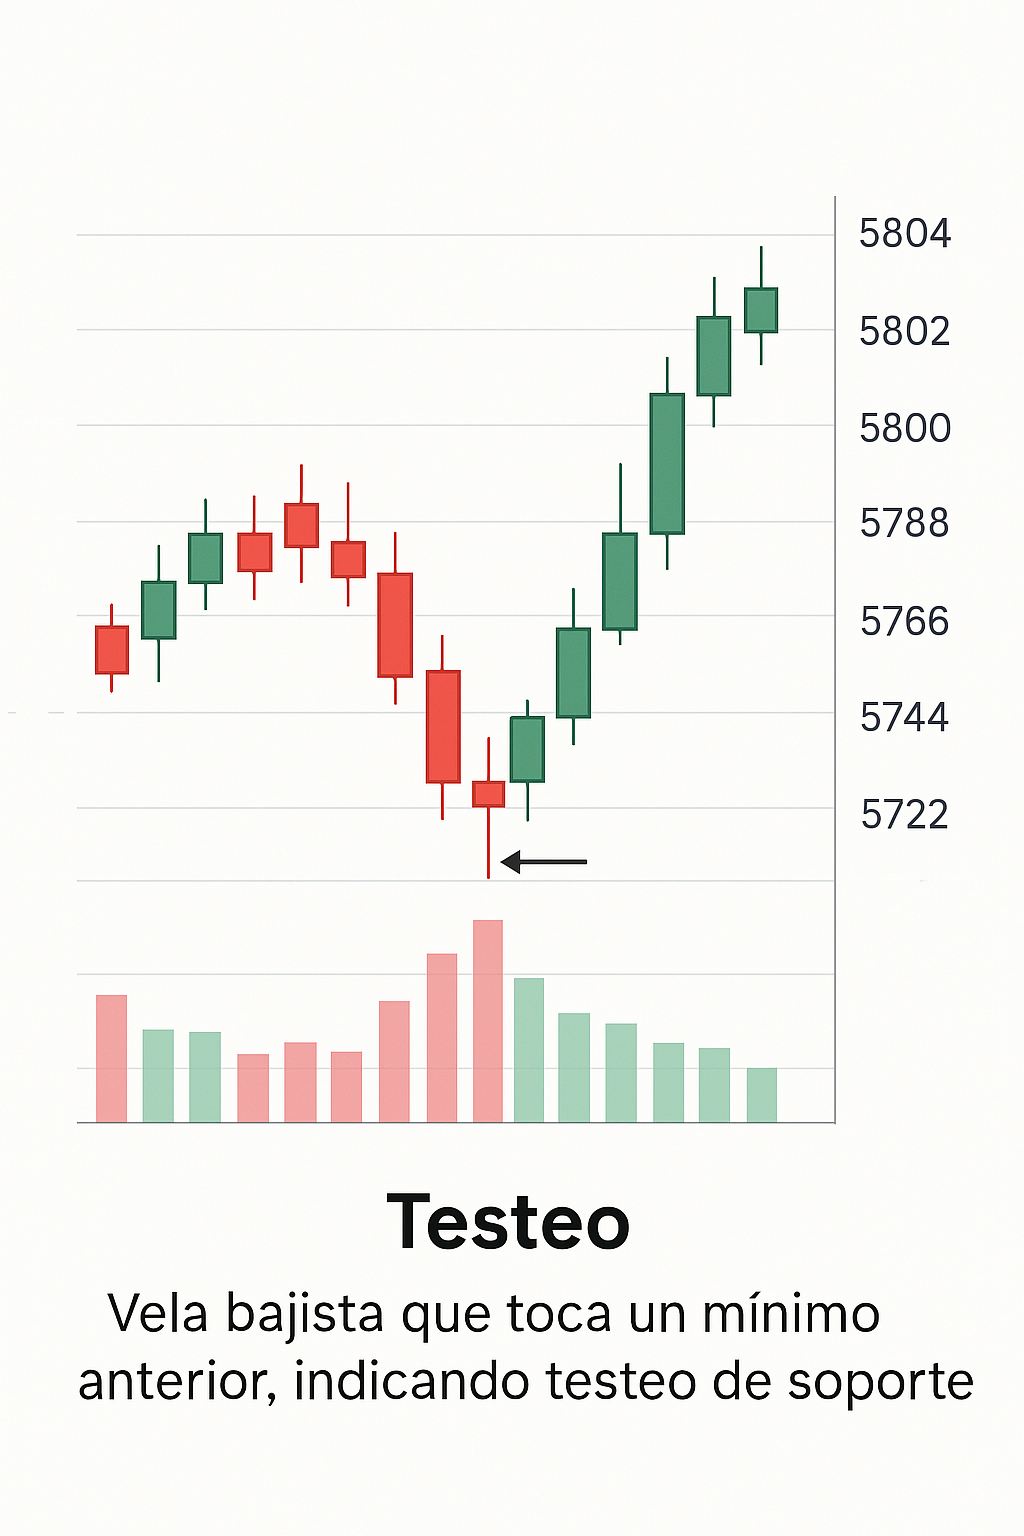
\includegraphics[width=11cm]{images/Testeo.png}
    \caption{Testeo}
    \label{fig:Testeo}
\end{figure}

En la figura \ref{fig:Testeo} ...

\subsection{Divergencia}

La \textbf{divergencia} se identifica por discordancias entre precio y volumen, indicando debilidad en la continuidad del movimiento:

\begin{itemize}
    \item Precio avanza, pero el volumen no lo respalda.
    \item Se busca en soportes, resistencias, directrices y zonas previamente operadas.
\end{itemize}

\begin{figure}[!htbp]
    \centering
    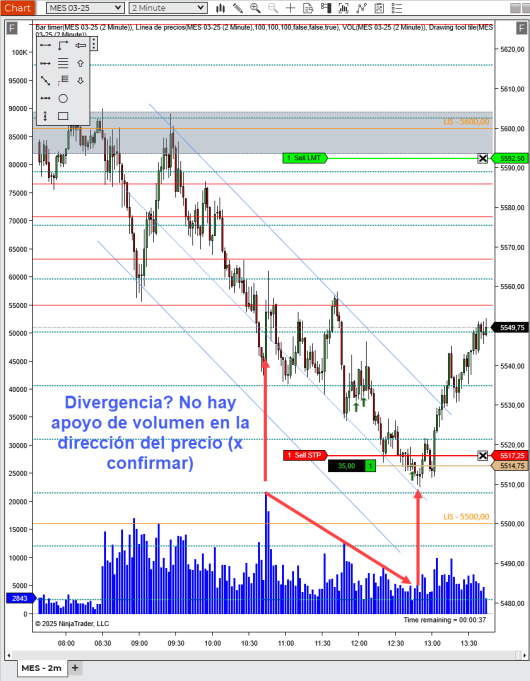
\includegraphics[width=11cm]{images/diver_1.png}
    \caption{Divergencia}
    \label{fig:diver_1}
\end{figure}

En la figura \ref{fig:diver_1} ...

\section{Fases y Estructuras del Profesional}

\subsection{Acumulaci\'on y Distribuci\'on}

\textbf{Acumulaci\'on}: compra institucional en un rango estrecho en la parte baja del gr\'afico.

\subsubsection*{Acumulaci\'on (Fase Profesional)}

\textbf{Descripci\'on textual:}

Proceso mediante el cual los operadores institucionales compran progresivamente en zonas de soporte, generalmente tras una fase de ca\'ida o correcci\'on prolongada. Se caracteriza por:

\begin{itemize}
    \item Movimiento lateral con m\'inimos similares.
    \item Volumen sostenido o creciente sin avance inmediato en el precio.
    \item Velas de rechazo alcista (\textit{pin bars}, \textit{engulfings}).
    \item Picos de volumen que coinciden con velas de rango estrecho o sombras inferiores largas.
\end{itemize}

\begin{figure}[!htbp]
    \centering
    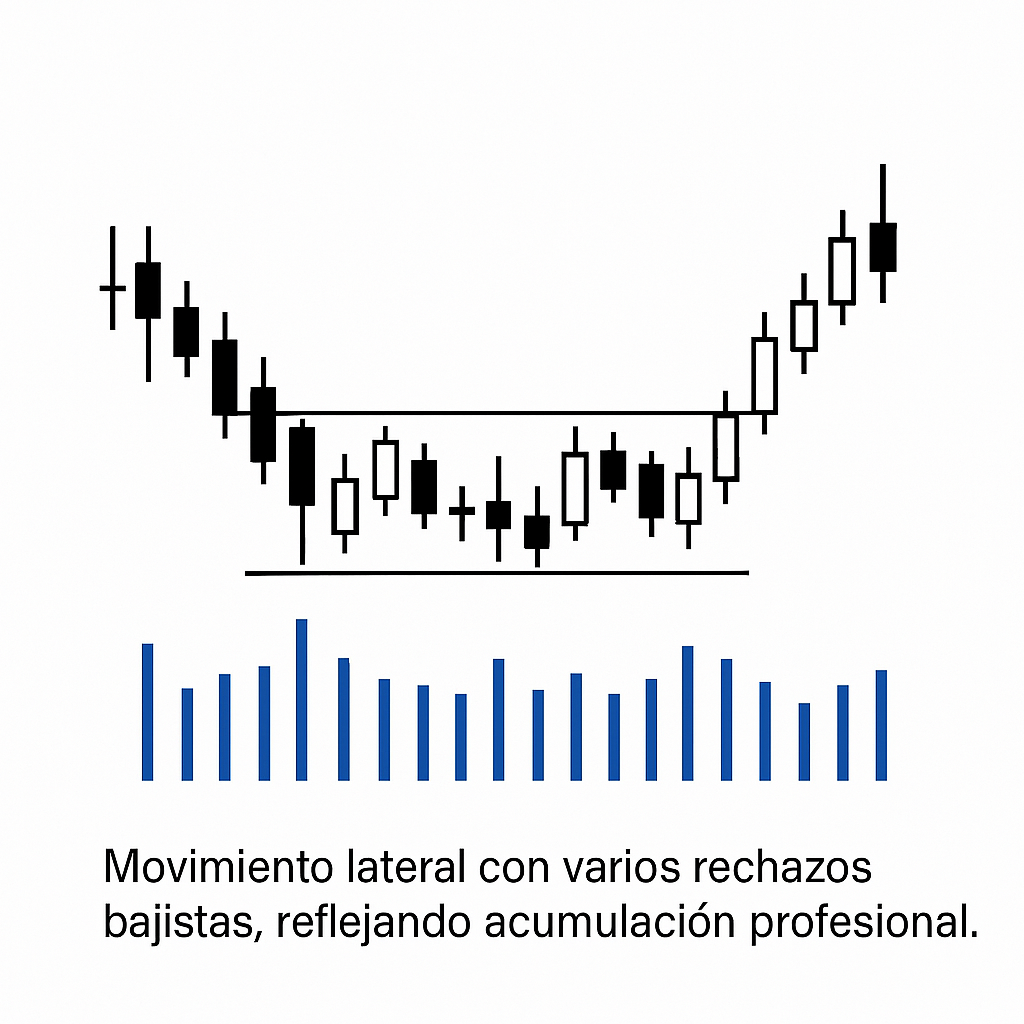
\includegraphics[width=11cm]{images/Acumulacion.png}
    \caption{Acumulaci\'on}
    \label{fig:Acumulacion}
\end{figure}

En la figura \ref{fig:Acumulacion} ...

\textbf{Distribuci\'on}: venta institucional en rangos estrechos en la parte alta del gr\'afico.
\subsubsection*{Distribuci\'on (Fase Profesional)}

\textbf{Descripci\'on textual:}

Proceso en el cual los operadores institucionales descargan posiciones (venden) en una zona de resistencia, generalmente tras una fase de tendencia alcista. Se caracteriza por:

\begin{itemize}
    \item Movimiento lateral con m\'aximos similares.
    \item Volumen alto sin progreso en el precio.
    \item Velas de rechazo bajista (\textit{pin bars}, \textit{engulfings}).
    \item Picos de volumen que coinciden con velas de cuerpo peque\~no o sombras superiores largas.
\end{itemize}

\begin{figure}[!htbp]
    \centering
    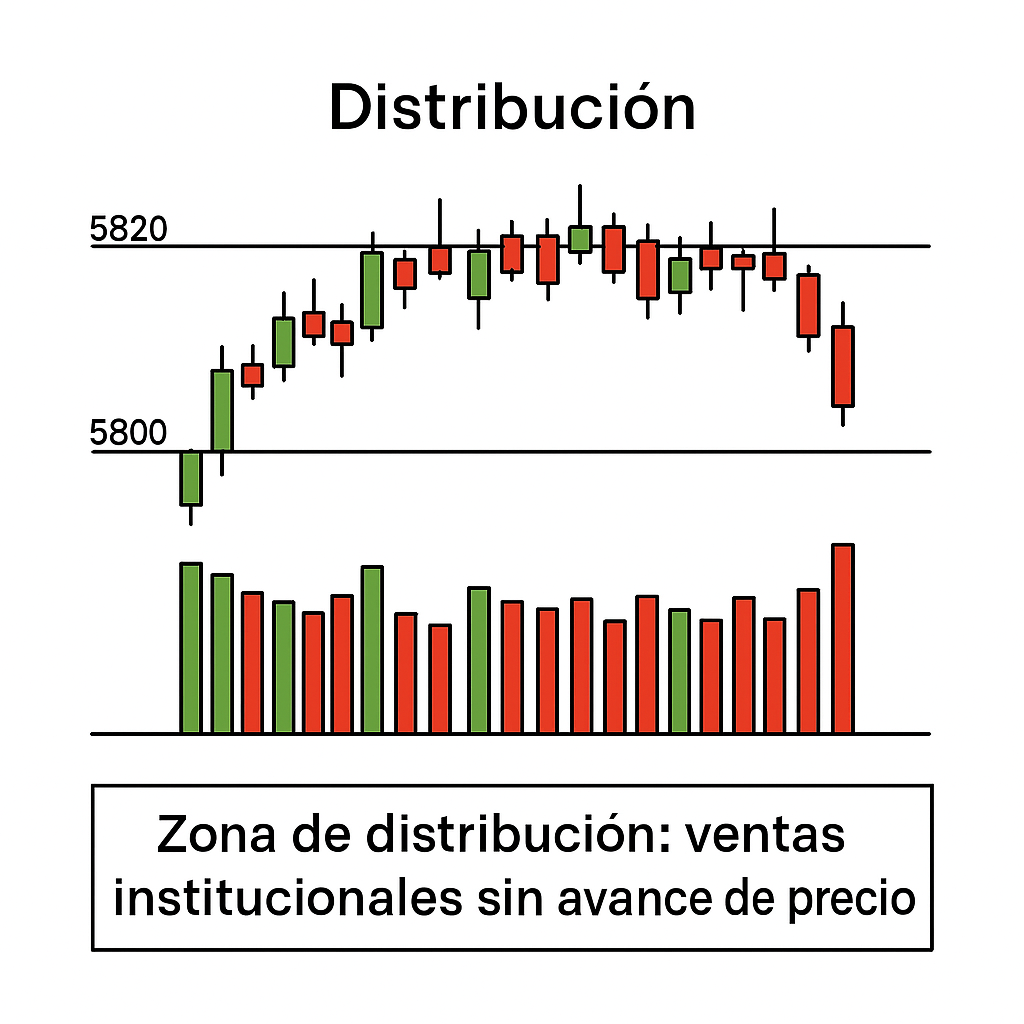
\includegraphics[width=11cm]{images/Distribucion.png}
    \caption{Distribuci\'on}
    \label{fig:Distribucion}
\end{figure}

En la figura \ref{fig:Distribucion} ...

Ambas fases implican una inversi\'on de tiempo y volumen significativos por parte del profesional, preparando movimientos posteriores mayores.

%\subsection{Caballo Ganador}

%Estructura fractal que combina impulsos y correcciones de distintos grados, todos en favor de un impulso principal. Sus claves:

%\begin{itemize}
%    \item Confirmaci\'on de cada subestructura por superaci\'on de niveles previos.
%    \item Objetivo: completar una segunda pata proporcional al impulso mayor.
%    \item Si una correcci\'on es superada, se confirma la continuaci\'on impulsiva.
%\end{itemize}

\section{An\'alisis de Velas}

El an\'alisis de velas, seg\'un Al Brooks, constituye una herramienta poderosa para entender la din\'amica subyacente del mercado, permitiendo interpretar la acci\'on del precio de manera profunda y eficaz. Brooks enfatiza la importancia del contexto, afirmando que ninguna vela debe analizarse de manera aislada; cada vela debe estudiarse considerando su posici\'on dentro de la tendencia global y el comportamiento precedente del precio.

\subsection{Velas de Intenci\'on}

Estas velas presentan un cuerpo amplio y cierran cerca de sus extremos superiores (si son alcistas) o inferiores (si son bajistas). Brooks considera que una vela de gran cuerpo refleja un sentimiento fuerte del mercado, con una clara dominancia por parte de compradores o vendedores. El volumen asociado a estas velas suele ser alto, indicando una fuerte participaci\'on institucional. Sin embargo, si una vela de intenci\'on aparece sin continuidad y con volumen decreciente, puede estar indicando una trampa o enga\~no de mercado.

\begin{figure}[!htbp]
    \centering
    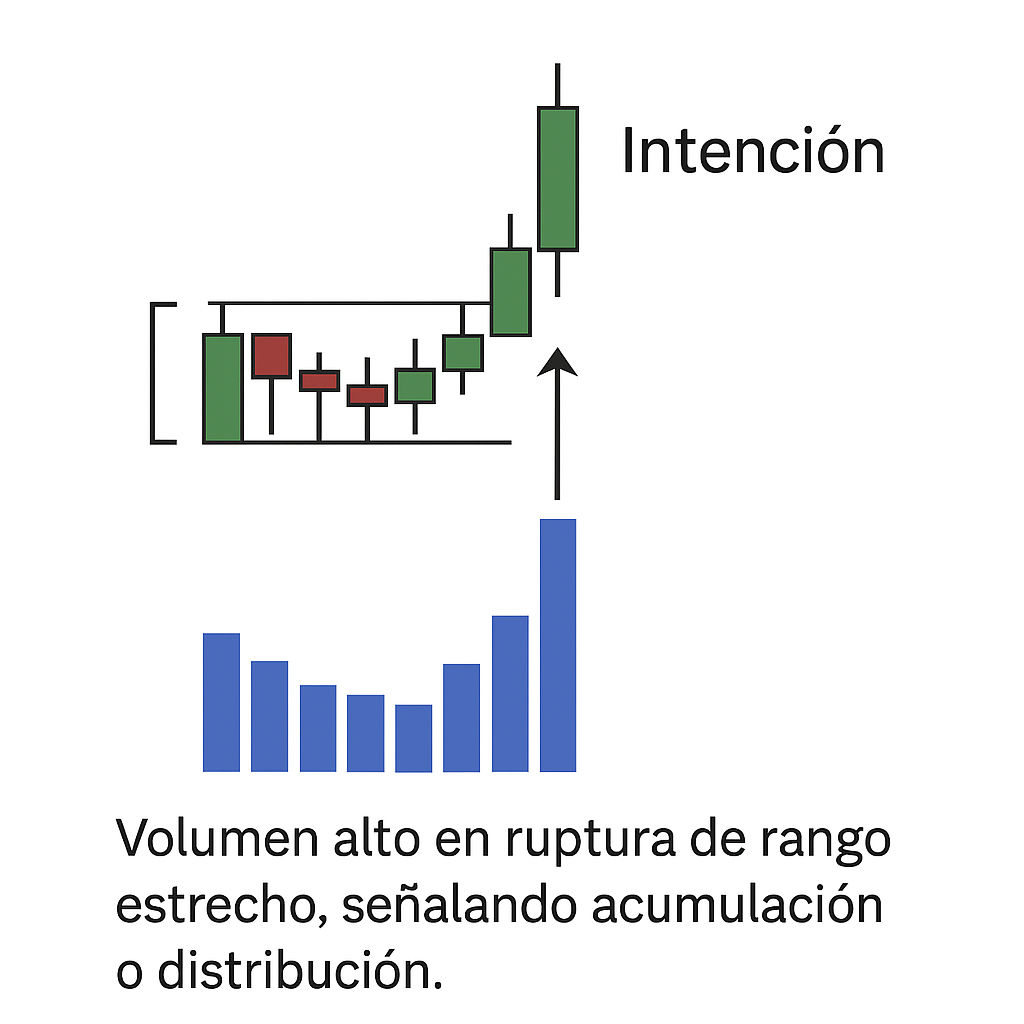
\includegraphics[width=11cm]{images/Intencion.png}
    \caption{Intenci\'on}
    \label{fig:Intencion2}
\end{figure}

En la figura \ref{fig:Intencion2} ...

\subsection{Velas Envolventes (Outside Bars)}

Una vela envolvente tiene un rango que excede tanto el m\'aximo como el m\'inimo de la vela anterior. Brooks indica que estas velas son complejas y deben analizarse con precauci\'on, pues pueden representar desde una pausa moment\'anea hasta un cambio de tendencia definitivo. Su relevancia aumenta considerablemente si aparecen tras movimientos prolongados, especialmente cuando capturan a operadores que entraron en velas anteriores, generando movimientos reactivos bruscos.

\begin{figure}[!htbp]
    \centering
    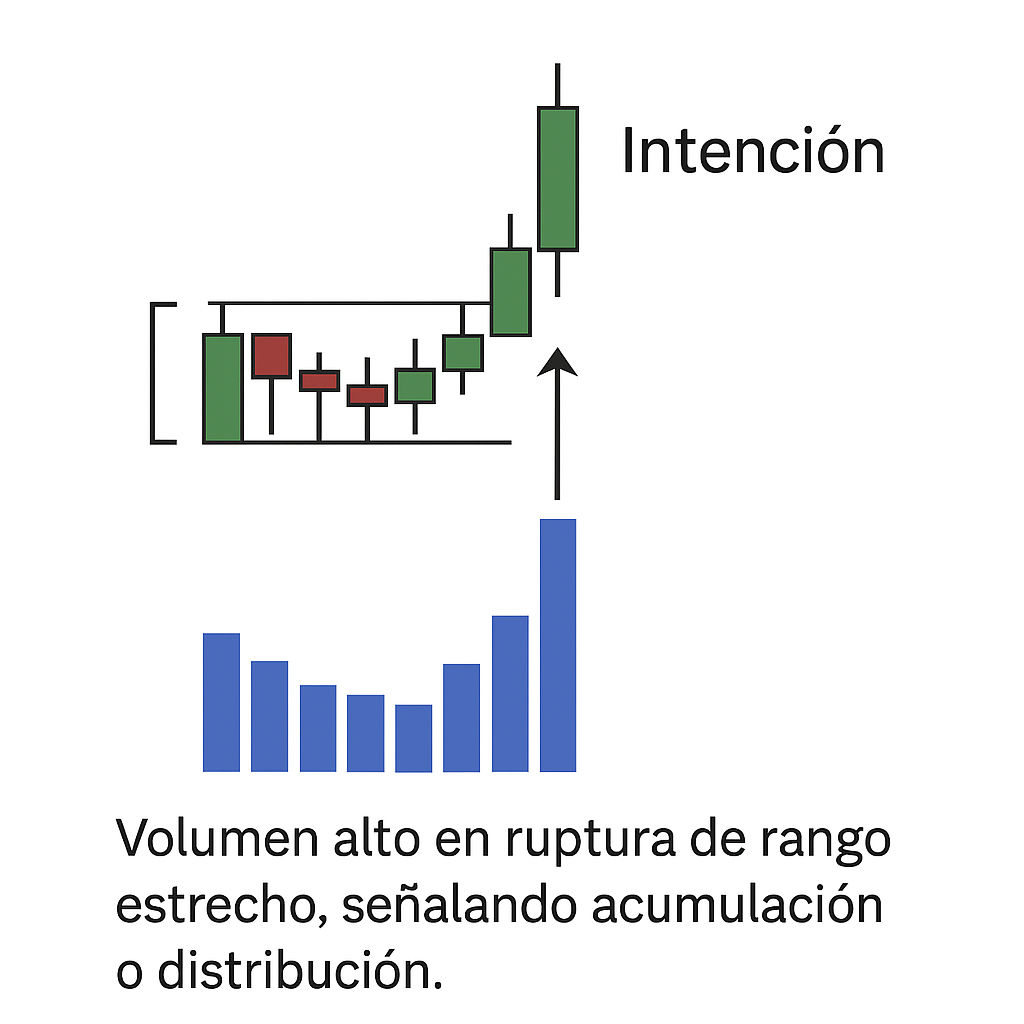
\includegraphics[width=11cm]{images/Intencion.png}
    \caption{Intenci\'on}
    \label{fig:Intencion3}
\end{figure}

En la figura \ref{fig:Intencion3} ...

\subsection{Velas de Rango Estrecho}

Estas velas, tambi\'en denominadas peonzas, muestran un cuerpo peque\~no y generalmente presentan mechas largas. Para Brooks, reflejan indecisi\'on o pausa, sugiriendo un agotamiento temporal de la fuerza impulsora predominante en el mercado. Cuando aparecen con volumen alto, son especialmente relevantes pues pueden indicar una absorci\'on significativa de \textit{oferta} o \textit{demanda}, alertando sobre posibles puntos de reversi\'on.

\subsection{Velas de Volumen Excesivo}

Caracterizadas por un cuerpo amplio acompa\~nado de un volumen extraordinariamente alto, estas velas a menudo esconden fuerza contraria. En una tendencia alcista, por ejemplo, una vela de este tipo podr\'ia implicar una distribuci\'on oculta por parte de operadores profesionales. Brooks recomienda analizar con cuidado estas velas dentro del contexto, especialmente en niveles extremos del gr\'afico.

\subsection{Velas Doji y Velas Inside}

Brooks se\~nala que las velas Doji, con apertura y cierre casi id\'enticos, representan una fuerte indecisi\'on del mercado. Cuando aparecen con volumen significativo, son potenciales precursoras de giros importantes. Las velas inside, contenidas completamente dentro del rango de la vela anterior, indican consolidaci\'on o equilibrio temporal. Pueden anticipar movimientos explosivos cuando son rotas con volumen elevado.

\subsection{Importancia del Contexto}

Al Brooks insiste en que el contexto define la validez de cualquier vela o patr\'on de velas. Una misma vela puede tener interpretaciones distintas seg\'un su ubicaci\'on dentro del ciclo del mercado. Por ejemplo, una vela envolvente en un mercado lateralizado tiene implicaciones diferentes a si ocurre tras una larga tendencia alcista o bajista.

\subsection{Integraci\'on con An\'alisis de Volumen}

Finalmente, es esencial validar la acci\'on del precio con volumen. Una vela alcista amplia debe estar respaldada por volumen alto para confirmar la intenci\'on profesional. Si el volumen es bajo, la vela podr\'ia ser una se\~nal falsa o manipulativa. Esta integraci\'on del an\'alisis de velas con el volumen es clave para la metodolog\'ia propuesta por Brooks, proporcionando un marco completo y robusto para la toma de decisiones operativas.

En resumen, el an\'alisis de velas seg\'un Al Brooks ofrece una visi\'on detallada y pragm\'atica para interpretar la din\'amica del mercado, enfatizando la importancia del contexto, el volumen y la acci\'on colectiva de las velas para anticipar movimientos futuros del precio.

\section{An\'alisis de Velas: Integrando los enfoques de Al Brooks y Miguel \'Angel Ram\'irez}

El an\'alisis de velas constituye una herramienta esencial para interpretar la acci\'on del precio. Tanto Miguel \'Angel Ram\'irez como Al Brooks enfatizan la importancia de estudiar la formaci\'on, estructura, volumen y contexto de las velas para detectar la intenci\'on profesional oculta detr\'as del movimiento del mercado.

Para ambos autores, las velas no deben interpretarse de forma aislada; es imprescindible considerar su contexto inmediato, la continuidad posterior al cierre y la relaci\'on con el volumen que las acompa\~na.

\subsection{La importancia del Contexto}

Al Brooks afirma que el significado de cada vela depende crucialmente de su ubicaci\'on en la estructura del mercado (tendencia, rango o transici\'on). Miguel \'Angel Ram\'irez, por su parte, coincide y enfatiza especialmente las \textbf{zonas relevantes} donde las velas adquieren mayor significaci\'on:

\begin{itemize}
    \item \textbf{Soportes y resistencias clave:} una vela alcista de intenci\'on con volumen alto en soporte revela acumulaci\'on profesional; en resistencia, una vela bajista de intenci\'on con alto volumen denota distribuci\'on.
    \item \textbf{Directrices mayores y menores:} velas que reaccionan claramente en estas l\'ineas de tendencia sugieren validaci\'on o ruptura profesional.
    \item \textbf{Patrones complejos (HCH, rangos laterales):} la ruptura o rechazo mediante velas de intenci\'on valida la presencia activa del profesional.
\end{itemize}

\subsection{Tipos de Velas y su interpretaci\'on operativa}

Al integrar ambos enfoques, se reconocen varios tipos espec\'ificos de velas y su significado desde la acci\'on profesional:

\subsubsection{Velas de Intenci\'on (Trend Bar - Brooks / Velas con Volumen Alto - Ram\'irez)}

Son velas con un cuerpo amplio, cierre en el extremo alto o bajo y con un volumen significativo. Ambas perspectivas coinciden en su interpretaci\'on:

\begin{itemize}
    \sloppy
    \item Indican clara dominancia de una de las fuerzas del mercado (compradores o vendedores).
    \item Son caracter\'isticas en rupturas genuinas de zonas relevantes (soportes, resistencias, directrices, rango).
    \item La ausencia inmediata de continuidad posterior puede indicar una trampa profesional (enga\~no).
\end{itemize}

Ejemplo: una vela grande alcista, que cierra cerca de m\'aximos y con alto volumen rompiendo un nivel relevante de resistencia, indica fuerte acumulaci\'on e intenci\'on profesional compradora. Sin embargo, si la siguiente vela revierte con volumen alto, puede indicar una trampa.

\subsubsection{Velas de Rango Estrecho o Peonzas}

Estas velas tienen cuerpos peque\~nos y volumen elevado. Seg\'un Ram\'irez, representan absorci\'on profesional; seg\'un Brooks, reflejan equilibrio temporal e indecisi\'on. Su interpretaci\'on conjunta es clara:

\begin{itemize}
    \item Indican pausa o potencial cambio de intenci\'on del mercado.
    \item La presencia de alto volumen confirma actividad profesional encubierta (acumulaci\'on o distribuci\'on oculta).
    \item Deben analizarse cuidadosamente en zonas relevantes, pues suelen anticipar movimientos explosivos posteriores.
\end{itemize}

Ejemplo: Una peonza con alto volumen en la parte alta de un rango indica posible distribuci\'on encubierta antes de una ca\'ida importante del mercado.

\subsubsection{Velas de Volumen Excesivo (Exhaustion Bar - Brooks)}

Seg\'un ambos autores, estas velas muestran cuerpos muy amplios con volumen exageradamente alto, indicando sobreesfuerzo y posible cl\'imax del movimiento vigente:

\begin{itemize}
    \item Brooks las describe como velas clim\'aticas, marcando agotamiento.
    \item Ram\'irez advierte que en niveles extremos pueden ocultar intenciones contrarias: los profesionales rara vez compran agresivamente en techos ni venden agresivamente en fondos.
    \item La falta de continuidad posterior confirma agotamiento y potencial giro del mercado.
\end{itemize}

Ejemplo: una vela clim\'atica alcista con volumen extremadamente alto tras una fuerte tendencia alcista puede se\~nalar distribuci\'on profesional previa a un giro bajista.

\subsection*{Puntos en Com\'un}

\begin{enumerate}
    \item \textbf{Aparici\'on tras movimientos prolongados:}
    \begin{itemize}
        \item Ambas velas suelen adquirir mayor relevancia cuando se presentan \textbf{al final de una tendencia fuerte}.
        \item En ese contexto, act\'uan como se\~nales potenciales de \textbf{cambio de fase}: transici\'on de tendencia a rango o reversi\'on.
    \end{itemize}

    \item \textbf{Lectura de agotamiento o trampa:}
    \begin{itemize}
        \item La \textbf{vela envolvente}, si no tiene continuaci\'on, puede reflejar \textbf{una trampa} o \textbf{absorci\'on profesional}.
        \item La \textbf{vela de volumen excesivo} tambi\'en sugiere un \textbf{cl\'imax de agotamiento}, donde los profesionales \textbf{capturan liquidez} de \textit{traders} minoristas.
    \end{itemize}

    \item \textbf{Advertencia de reversi\'on inminente:}
    \begin{itemize}
        \item Ambas velas pueden se\~nalar que el \textbf{movimiento vigente est\'a maduro o agotado}, y que existe un riesgo elevado de giro.
        \item En especial si van seguidas de falta de continuaci\'on o de una vela contraria fuerte.
    \end{itemize}

    \item \textbf{Necesidad de validaci\'on contextual:}
    \begin{itemize}
        \item Ni la vela envolvente ni la de volumen excesivo deben operar por s\'i solas: su interpretaci\'on requiere el \textbf{an\'alisis del contexto estructural y del volumen}.
        \item Ambas pueden fallar si se interpretan fuera de zonas relevantes (resistencias, soportes, extremos de canales).
    \end{itemize}

    \item \textbf{Captura de operadores mal posicionados:}
    \begin{itemize}
        \item Las dos velas suelen estar asociadas a \textbf{movimientos que atrapan} a quienes entraron tarde, lo que genera \textbf{reacciones violentas} en sentido contrario.
    \end{itemize}
\end{enumerate}

\subsection*{Conclusi\'on}

Ambos tipos de velas deben ser interpretados como \textbf{manifestaciones del comportamiento profesional} al final de un tramo de mercado. Aunque se enfocan en aspectos distintos (estructura vs.\ volumen), \textbf{convergen en su utilidad como se\~nales de agotamiento, manipulaci\'on o transici\'on}, especialmente en zonas t\'ecnicas clave.


\subsubsection{Velas de Rechazo (Reversal Bar - Brooks)}

Estas velas presentan largas sombras superiores o inferiores y cuerpo peque\~no a medio. Para Ram\'irez, estas velas aparecen en «testeos» para comprobar la presencia contraria. Para Brooks, significan un claro rechazo a un nivel espec\'ifico:

\begin{itemize}
    \item Una sombra inferior larga en un soporte relevante indica rechazo a precios m\'as bajos y posible comienzo de acumulaci\'on profesional.
    \item Una sombra superior larga en resistencia relevante denota rechazo de precios altos y posible inicio de distribuci\'on profesional.
    \item La confirmaci\'on mediante la siguiente vela es fundamental para validar o descartar la reversi\'on del movimiento.
\end{itemize}

Ejemplo: una vela bajista con sombra inferior muy larga sobre un soporte importante, seguida de una vela alcista de intenci\'on con volumen, indica acumulaci\'on validada y giro alcista.

\subsection{Integraci\'on operativa: Precio y Volumen}

La integraci\'on del volumen en el an\'alisis de velas potencia enormemente la capacidad predictiva del trader:

\begin{itemize}
    \item Las velas de intenci\'on deben ir acompa\~nadas siempre de volumen alto para ser consideradas v\'alidas; ausencia de volumen implica falsa ruptura o trampa profesional.
    \item Velas de rango estrecho con volumen alto indican absorci\'on profesional, anticipando movimientos significativos.
    \item Las velas clim\'aticas (excesivas) siempre tienen volumen exagerado, confirmando agotamiento.
\end{itemize}

Ambos enfoques coinciden plenamente en que el volumen aporta confirmaci\'on y seguridad operativa.

\subsection{Confirmaci\'on y Continuidad}

Para Brooks y Ram\'irez es clave la continuidad posterior a cualquier vela relevante:

\begin{itemize}
    \item Una vela fuerte (intenci\'on) requiere continuidad inmediata; su ausencia sugiere una trampa.
    \item Las velas de rechazo deben ser seguidas de velas confirmatorias en direcci\'on contraria al rechazo.
    \item Velas clim\'aticas deben mostrar rechazo inmediato al movimiento previo para confirmar el agotamiento.
\end{itemize}

\subsection{Conclusi\'on Integradora}

La combinaci\'on de las perspectivas de Al Brooks y Miguel \'Angel Ram\'irez en el an\'alisis de velas proporciona un enfoque potente y detallado para interpretar adecuadamente el mercado. Al observar la interacci\'on entre contexto, fuerza relativa (forma y tama\~no), continuidad y volumen, el trader obtiene una lectura clara de las verdaderas intenciones profesionales, logrando as\'i anticiparse a movimientos importantes y evitando trampas comunes en los mercados financieros.

Este an\'alisis profundo permite al operador actuar del lado correcto del mercado, alineado con las fuerzas institucionales y aumentando significativamente sus probabilidades de \'exito.

\section{Zonas Relevantes: Profundizaci\'on Operativa}

Las \textbf{zonas relevantes} constituyen niveles clave donde la interacci\'on del precio y el volumen revela con claridad la actividad profesional y permite tomar decisiones operativas precisas. Miguel \'Angel Ram\'irez y Al Brooks enfatizan que el correcto reconocimiento y an\'alisis de estas zonas representa uno de los pilares fundamentales del trading profesional basado en la acci\'on del precio.

Estas zonas no son simples l\'ineas est\'aticas, sino \textbf{\'areas din\'amicas} donde la lucha entre oferta y demanda genera patrones espec\'ificos y reveladores.

\subsection{Soportes y Resistencias Clave}

Seg\'un ambos autores, soportes y resistencias relevantes no son niveles fijos, sino rangos donde los profesionales han demostrado inter\'es significativo, ya sea mediante acumulaci\'on (compras institucionales) o distribuci\'on (ventas institucionales):

\begin{itemize}
    \item \textbf{Soporte relevante:} Un nivel o rango inferior del gr\'afico en el que, reiteradamente, el precio ha detenido su descenso. La presencia profesional se revela mediante velas de rechazo con volumen alto o testeos con secado de volumen.
    
    \item \textbf{Resistencia relevante:} Nivel o rango superior donde el precio repetidamente se ha detenido en su ascenso. Suele revelarse mediante velas de rechazo bajista, velas de rango estrecho con volumen alto (absorci\'on) o secado posterior a testeos alcistas fallidos.
    
    \item \textbf{Validaci\'on del nivel relevante:} Seg\'un Ram\'irez, un soporte recuperado con volumen e intenci\'on es la se\~nal m\'as clara de fortaleza. De manera an\'aloga, una resistencia dilatada con volumen sugiere clara debilidad y posible reversi\'on bajista.
\end{itemize}

\vspace{1em}
\noindent

\begin{figure}[!htbp]
    \centering
    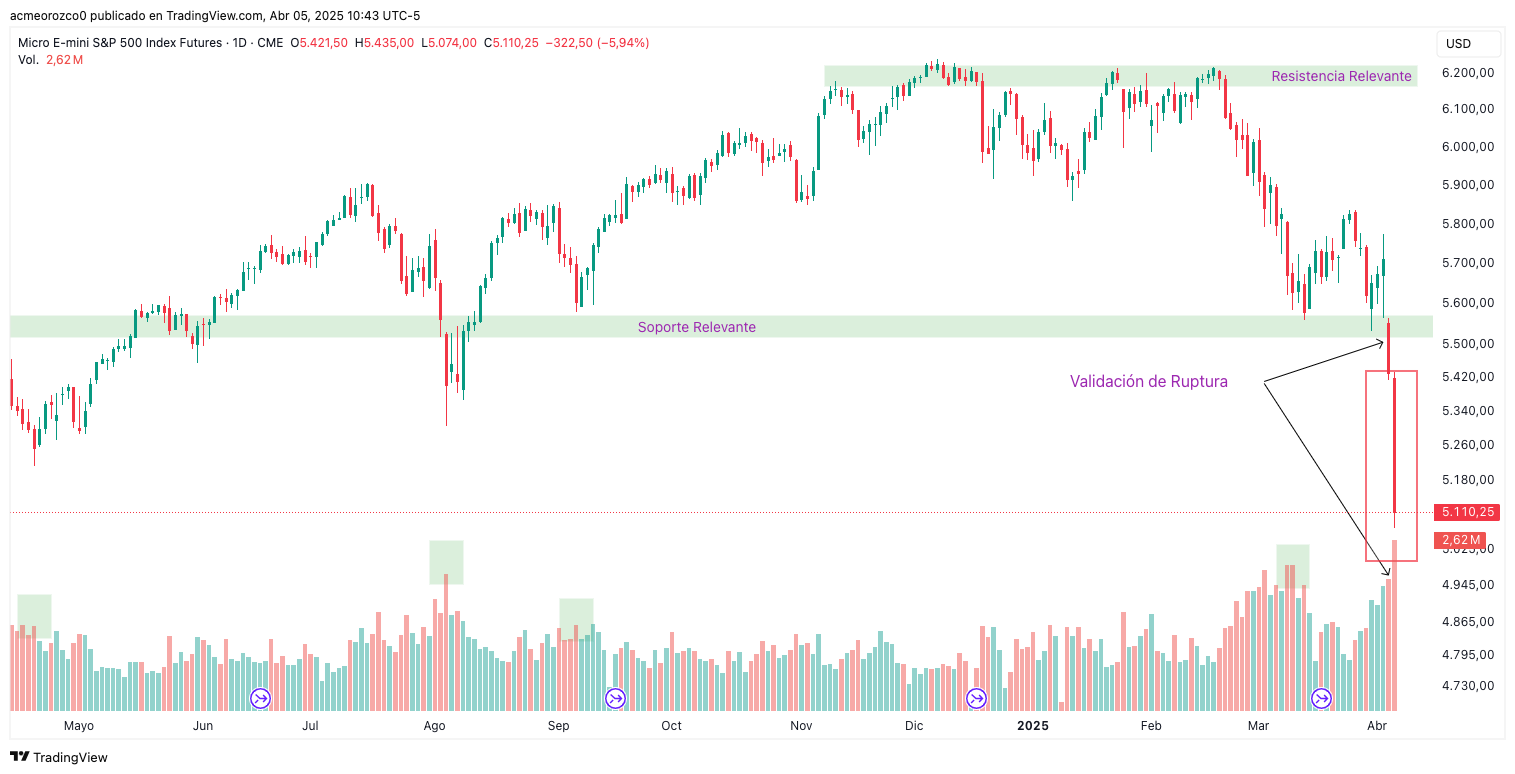
\includegraphics[width=11cm]{images/soportes_resistencias_validacion.png}
    \caption{Soporte, Resistencia y validaci\'on de Ruptura de Zona Clave}
    \label{fig:soportes_resistencias_validacion}
\end{figure}
\vspace{0.5em}
\noindent

\subsection{Interpretaci\'on del Gr\'afico, figura \ref{fig:soportes_resistencias_validacion}: Soportes, Resistencias y Validaci\'on}

La imagen anotada representa visualmente el concepto de \textbf{Soportes y Resistencias Clave}, aplicado al contrato diario del \textbf{MES-0625 (Micro E-mini S\&P 500 Futures)}. A continuaci\'on se detalla la lectura t\'ecnica de cada elemento:

\subsubsection*{Soporte relevante}

\textbf{Ubicaci\'on:} Zona horizontal entre 5.570 y 5.500 puntos, marcada con un recuadro verde con la anotaci\'on ``Soporte Relevante''.

\begin{itemize}
    \item Esta \'area muestra varios \textbf{rebotes del precio} tras ca\'idas, indicando la presencia de demanda institucional.
    \item Es una regi\'on donde se ha evidenciado \textbf{acumulaci\'on profesional}, seg\'un Ram\'irez, observable por:
    \begin{itemize}
        \item Velas con sombras inferiores largas (rechazo del precio a seguir cayendo).
        \item Incremento del volumen en los rebotes.
    \end{itemize}
    \item Act\'ua como \textbf{zona de defensa} del mercado: cada contacto del precio con esta zona activa la intervenci\'on de compradores profesionales.
\end{itemize}

\subsubsection*{Resistencia relevante}

\textbf{Ubicaci\'on:} Rango entre 6.150 y 6.220 puntos, señalado con un recuadro verde.

\begin{itemize}
    \item Este nivel funciona como techo t\'ecnico, deteniendo el avance del precio en m\'ultiples ocasiones.
    \item Se observa \textbf{distribuci\'on profesional} por medio de:
    \begin{itemize}
        \item Velas de rango estrecho con volumen alto (absorci\'on).
        \item Rechazos bajistas tras testeos fallidos.
    \end{itemize}
    \item La incapacidad del precio de mantenerse por encima de esta zona refuerza su condici\'on de resistencia clave.
\end{itemize}

\subsubsection*{Validaci\'on bajista del soporte}

\textbf{Ubicaci\'on:} Vela del 4 de abril de 2025, marcada con un recuadro rojo.

\begin{itemize}
    \item Se trata de una \textbf{vela bajista de cuerpo amplio}, con un volumen excepcional de \textbf{2{,}62 millones de contratos}.
    \item Representa una \textbf{ruptura con intenci\'on} del soporte, seg\'un el criterio de Miguel \'Angel Ram\'irez.
    \item El movimiento vertical y la falta de rechazo sugieren \textbf{dominancia de la oferta institucional}.
    \item Esto valida la \textbf{debilidad del nivel}, abriendo paso a una fase tipo \textit{markdown}.
\end{itemize}

\subsubsection*{Conclusi\'on operativa}

Este gr\'afico constituye un ejemplo pr\'actico del modelo de lectura institucional:

\begin{itemize}
    \item Identificaci\'on de zonas de inter\'es profesional (soporte y resistencia).
    \item Observaci\'on del comportamiento del precio ante dichos niveles.
    \item Confirmaci\'on mediante \textbf{intenci\'on y volumen} para validar rupturas o rechazos.
\end{itemize}

Este tipo de lectura permite al operador alinear sus decisiones con el flujo profesional del mercado.

\subsection{L\'ineas de Tendencia (Directrices)}

Al Brooks resalta la importancia operativa de las l\'ineas de tendencia como zonas din\'amicas, mientras Ram\'irez se enfoca en identificar la intenci\'on profesional en estas directrices:

\begin{itemize}
    \item Una l\'inea de tendencia efectiva conecta m\'ultiples puntos donde los profesionales actuaron previamente (acumulaci\'on o distribuci\'on).
    
    \item Para que una ruptura de directriz sea fiable, debe hacerse con \textbf{intenci\'on}: vela de amplio rango, cierre decidido m\'as all\'a de la directriz y aumento significativo del volumen. De lo contrario, se trata de un testeo o dilataci\'on (trampa profesional).
    
    \item Una l\'inea de tendencia rota con intenci\'on revela cambios potencialmente profundos en la estructura del mercado, indicando transici\'on desde una fase impulsiva a correctiva o viceversa.
\end{itemize}

\subsubsection{L\'ineas de Tendencia (Directrices) en el MES-0625}

En la siguiente imagen, \ref{fig:lineas_tendencia_directrices}, se ilustran dos \textbf{directrices clave} que reflejan la acci\'on institucional sobre el contrato \textbf{MES-0625} en el marco diario, junto con una \textbf{ruptura con intenci\'on} que valida un cambio estructural del mercado:


\vspace{1em}
\noindent

\begin{figure}[!htbp]
    \centering
    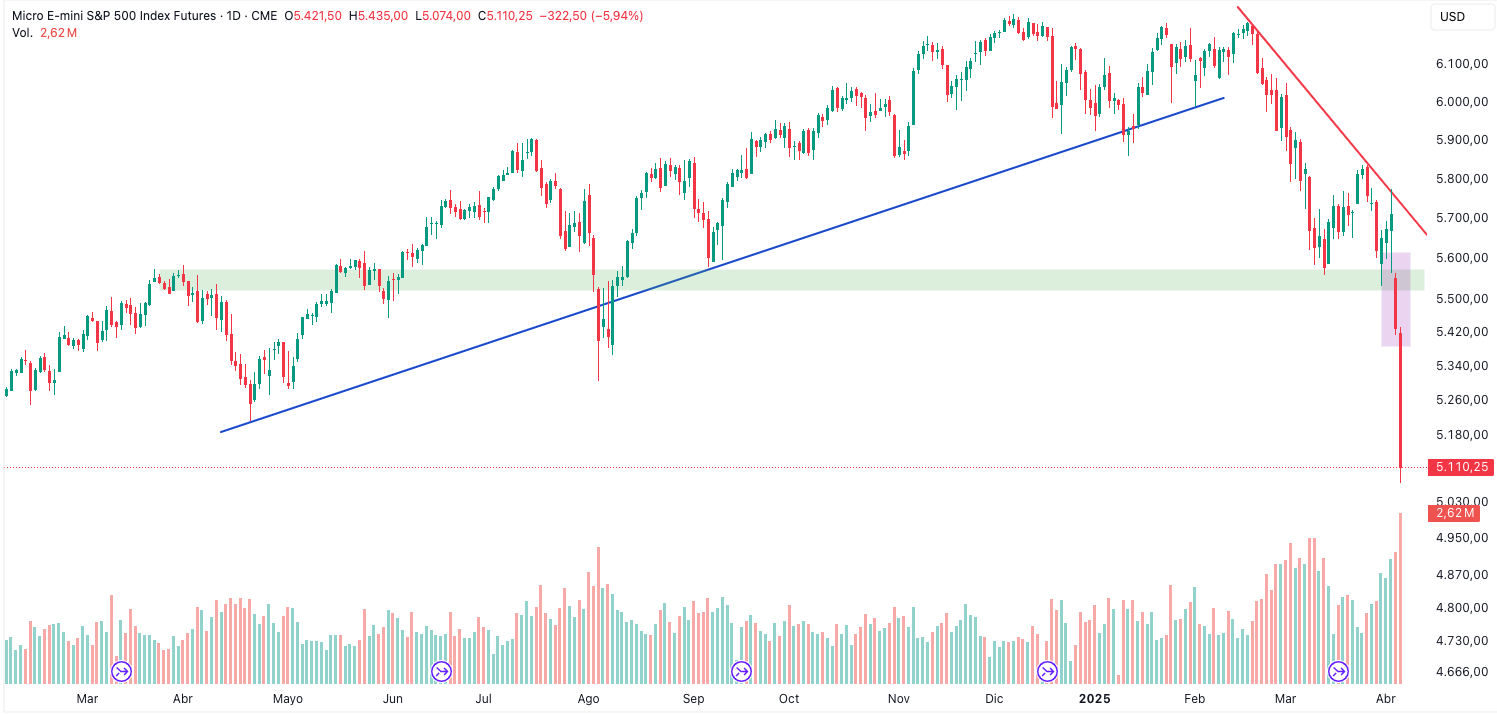
\includegraphics[width=11cm]{images/lineas_tendencia_directrices.png}
    \caption{L\'ineas de Tendencia (Directrices) en el MES-0625 y Ruptura de Zona Clave}
    \label{fig:lineas_tendencia_directrices}
\end{figure}
\vspace{0.5em}
\noindent

\begin{itemize}
    \item \textbf{Directriz alcista (azul):} conecta los m\'inimos ascendentes desde octubre de 2023 hasta abril de 2024. Esta l\'inea representa una fase de \textbf{acumulaci\'on profesional}, donde la demanda institucional sosten\'ia el mercado. Su pendiente refleja una estructura de m\'inimos crecientes, t\'ipica de una fase impulsiva alcista.
    
    \item \textbf{Directriz bajista (roja):} une los m\'aximos descendentes desde inicios de 2025 hasta marzo–abril del mismo a\~no. Esta estructura indica una fase de \textbf{distribuci\'on}, donde la oferta comienza a dominar lentamente el mercado, frenando los impulsos alcistas y anticipando un giro.
    
    \item \textbf{Ruptura con intenci\'on (recuadro morado):} el 4 de abril de 2025 se observa una \textbf{vela de amplio rango bajista} que rompe de forma decidida el soporte relevante. Esta vela est\'a acompa\~nada por un volumen hist\'oricamente alto (2{,}62 millones de contratos), cumpliendo con los criterios de Ram\'irez para validar una ruptura con intenci\'on:
    \begin{itemize}
        \item Cuerpo amplio y direccional.
        \item Cierre por debajo de la directriz.
        \item Volumen extraordinario.
    \end{itemize}
    Esta ruptura sugiere el paso desde una fase de \textbf{distribuci\'on} a una \textbf{fase impulsiva bajista} o \textit{markdown}.
\end{itemize}

\vspace{1em}
\noindent
Este tipo de lectura sobre las directrices permite anticipar cambios de fase del mercado y validar la presencia profesional en zonas clave, fortaleciendo la estrategia operativa basada en acci\'on del precio y volumen.


\subsection{Patrones Complejos y Zonas Claviculares}

Miguel \'Angel Ram\'irez enfatiza la importancia de los \textbf{patrones complejos}, como el Hombro-Cabeza-Hombro (HCH), dobles techos y estructuras compuestas, como manifestaciones t\'ipicas de \textbf{distribuci\'on o acumulaci\'on profesional} en zonas t\'ecnicas clave. En este marco, el concepto de \textbf{zona clavicular} adquiere un rol operativo fundamental.

\begin{itemize}
    \item La \textbf{clavicular} es una l\'inea que conecta los \textbf{m\'inimos en patrones alcistas} o los \textbf{m\'aximos en patrones bajistas}, actuando como \textbf{nivel din\'amico de equilibrio} entre oferta y demanda. En t\'erminos funcionales, representa la frontera que, una vez rota con convicci\'on, habilita desplazamientos impulsivos.

    \item La clavicular conecta puntos cr\'iticos (m\'inimos en patrones alcistas o m\'aximos en bajistas), formando niveles din\'amicos clave.  
    \item Una ruptura clara de la clavicular con volumen alto valida el patr\'on y anticipa movimientos de gran amplitud. Ausencia de volumen sugiere falsa ruptura o testeo fallido.    
    \item Ram\'irez recomienda trazar la clavicular no solo en el grado mayor, sino tambi\'en en el grado menor m\'as reciente, aumentando la precisi\'on operativa.
    \item Una \textbf{ruptura con volumen alto e intenci\'on clara} valida el patr\'on y suele anticipar movimientos amplios y definidos. Este elemento es esencial para distinguir entre una \textbf{ruptura genuina} y una \textbf{falsa ruptura} o \textit{trampa institucional}, cuando la acci\'on carece de volumen o continuidad.
    \item Ram\'irez propone un an\'alisis multigrado: no basta con trazar la clavicular en el patr\'on visible de mayor jerarqu\'ia, sino que tambi\'en debe identificarse la \textbf{clavicular del patr\'on interno m\'as reciente}. Esta pr\'actica permite:
    \begin{itemize}
        \item Mejorar la \textbf{precisi\'on en las entradas}.
        \item Detectar anticipadamente \textbf{fallos estructurales} o \textbf{confirmaciones operativas}.
    \end{itemize}
    \item Las zonas claviculares tambi\'en permiten evaluar el \textbf{rol de testeo}, ya que un retroceso hacia la clavicular rota puede validar la ruptura si se acompa\~na de secado de volumen o rechazo (intenci\'on inversa).
    \item Las zonas claviculares tambi\'en son v\'alidas como \textbf{zonas de testeo posterior a la ruptura}. Un retroceso controlado hacia la clavicular rota, con \textbf{secado de volumen o rechazo}, puede confirmar la intenci\'on profesional y habilitar una entrada en favor del movimiento validado.
\end{itemize}

\noindent
Este abordaje profundo de las zonas claviculares se integra al enfoque institucional de Ram\'irez, quien no las utiliza como patrones autom\'aticos, sino como \textbf{zonas vivas}, en las que la lectura del volumen, el contexto previo y la continuidad posterior determinan su validez como punto de transici\'on estructural.

\vspace{1em}
\noindent
\begin{figure}[!htbp]
    \centering
    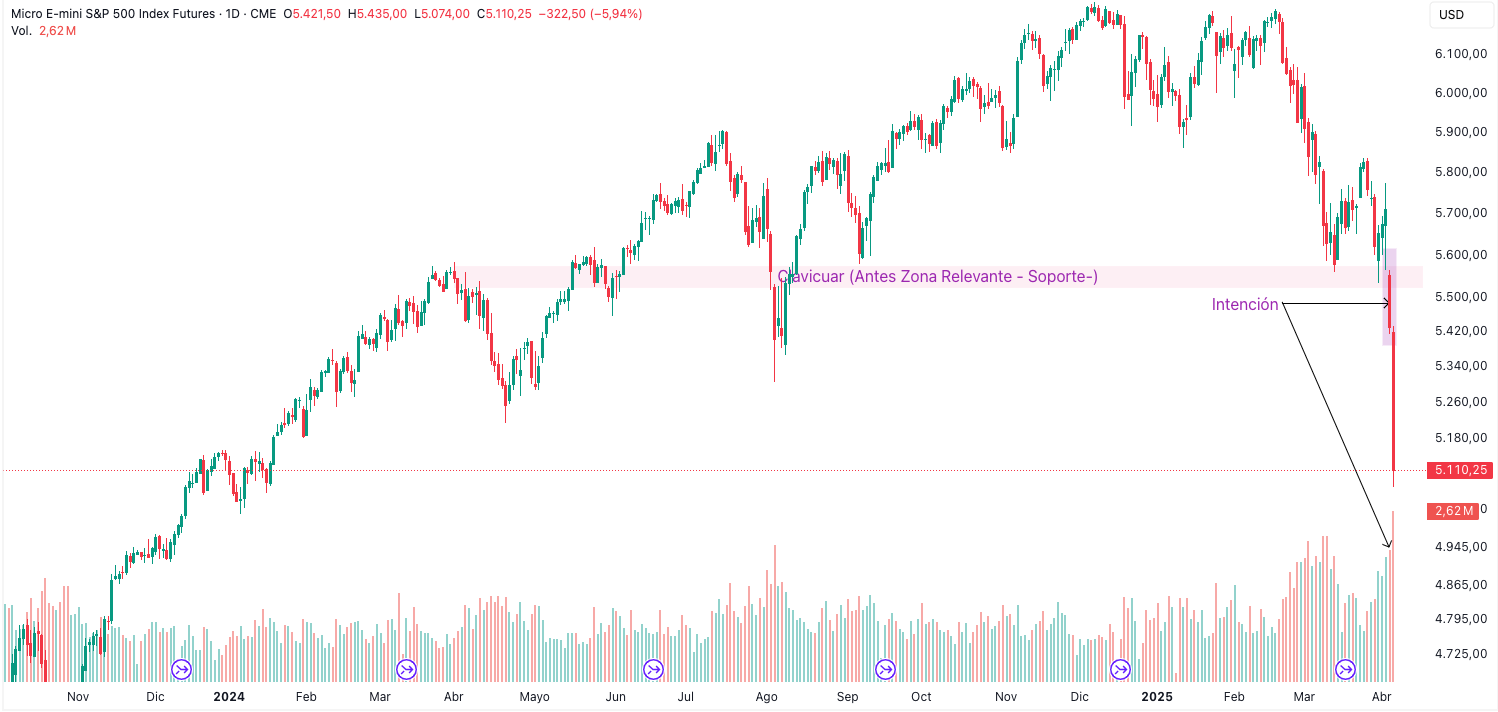
\includegraphics[width=11cm]{images/patrones_claviculares_test_ruptura.png}
    \caption{Estructura de clavicular, testeo previo y ruptura con volumen en el MES-0625}
    \label{fig:patrones_claviculares_test_ruptura}
\end{figure}
\vspace{0.5em}
\noindent


En la figura \ref{fig:patrones_claviculares_test_ruptura} se observa un ejemplo operativo del concepto de \textbf{zonas claviculares} aplicado al contrato \textbf{MES-0625} en marco diario. La estructura muestra un patr\'on complejo tipo Hombro-Cabeza-Hombro, seguido de una ruptura validada por volumen. Se identifican los siguientes elementos:

\begin{itemize}
    \item \textbf{Clavicular:} traza la l\'inea que conecta los m\'inimos clave de la estructura completa, actuando como frontera principal entre la fase de distribuci\'on y el potencial movimiento impulsivo bajista.

    \item \textbf{Testeo:} antes de la ruptura definitiva, el precio realiza un retroceso que pone a prueba la zona clavicular, valid\'andola mediante rechazo con bajo volumen.

    \item \textbf{Ruptura con Volumen:} la vela del 4 de abril de 2025 rompe la clavicular (antes Zona Relevante ---Soporte--- ) con cuerpo amplio y volumen hist\'orico (2{,}62 millones de contratos), confirmando la intenci\'on institucional y validando el patr\'on bajista.
\end{itemize}

\noindent
Este tipo de lectura secuencial permite detectar y operar transiciones estructurales reales, evitando falsas rupturas y posicionando al operador en sincron\'ia con la acci\'on profesional del mercado.


\subsection{Zonas de Acumulaci\'on y Distribuci\'on}

Estas zonas son centrales en el an\'alisis de Ram\'irez y respaldadas indirectamente por Brooks mediante su interpretaci\'on contextual:

\begin{itemize}
    \item \textbf{Zonas de Acumulaci\'on:} Identificadas en la parte baja del gr\'afico, caracterizadas por movimientos laterales con volumen alto en velas de rango estrecho (absorci\'on). La salida alcista posterior, con velas de intenci\'on y volumen relevante, confirma la acumulaci\'on previa. Ram\'irez describe estas zonas como estructuras laterales que se forman tras prolongadas ca\'idas, usualmente en la parte baja del gr\'afico. En ellas, el operador profesional \textbf{absorbe oferta} mediante velas de rango estrecho y volumen elevado. La salida posterior mediante velas de intenci\'on con volumen creciente valida dicha acumulaci\'on. Este enfoque coincide con la lectura contextual de Brooks, quien se enfoca en \textbf{rangos en la base con ruptura impulsiva y continuidad}.
    
    \item \textbf{Zonas de Distribuci\'on:} Encontradas en la parte alta del gr\'afico, con movimientos laterales similares pero con actividad vendedora oculta. Confirmadas cuando aparecen velas bajistas fuertes con alto volumen rompiendo soportes internos del rango lateral. Estas estructuras se configuran en los techos del mercado. Seg\'un Ram\'irez, el profesional \textbf{vende sin mover el precio}, generando una aparente lateralidad. La ruptura bajista posterior, con volumen alto y velas de amplio rango, confirma la distribuci\'on. Brooks, desde su an\'alisis de rango y reversi\'on en extremos, tambi\'en reconoce este comportamiento, aunque lo interpreta desde el \textbf{cambio de probabilidad en zonas de resistencia}.
    
    \item \textbf{Duraci\'on y volumen acumulado:} Ram\'irez enfatiza que \textbf{a mayor duraci\'on y volumen en la fase de acumulaci\'on o distribuci\'on}, mayor ser\'a la energ\'ia liberada una vez se valide la ruptura. Este principio est\'a vinculado con la \textbf{ley de causa y efecto}, y se proyecta directamente en la magnitud del desplazamiento posterior. Brooks, por su parte, indica que \textbf{cuanto m\'as testado un rango, m\'as fuerte suele ser su ruptura si hay confirmaci\'on de volumen e intenci\'on}. Cuanto mayor es el tiempo y volumen invertido en acumulaci\'on o distribuci\'on, m\'as potente ser\'a el movimiento resultante una vez que se rompa definitivamente dicha zona.
\end{itemize}

\noindent
Esta integraci\'on te\'orica refuerza la utilidad operativa de estas zonas como puntos estructurales clave, donde la lectura combinada de \textbf{volumen, acci\'on del precio y continuidad} permite identificar de manera anticipada la participaci\'on profesional y proyectar movimientos de alta probabilidad.


\vspace{1em}
\noindent
\begin{figure}[!htbp]
    \centering
    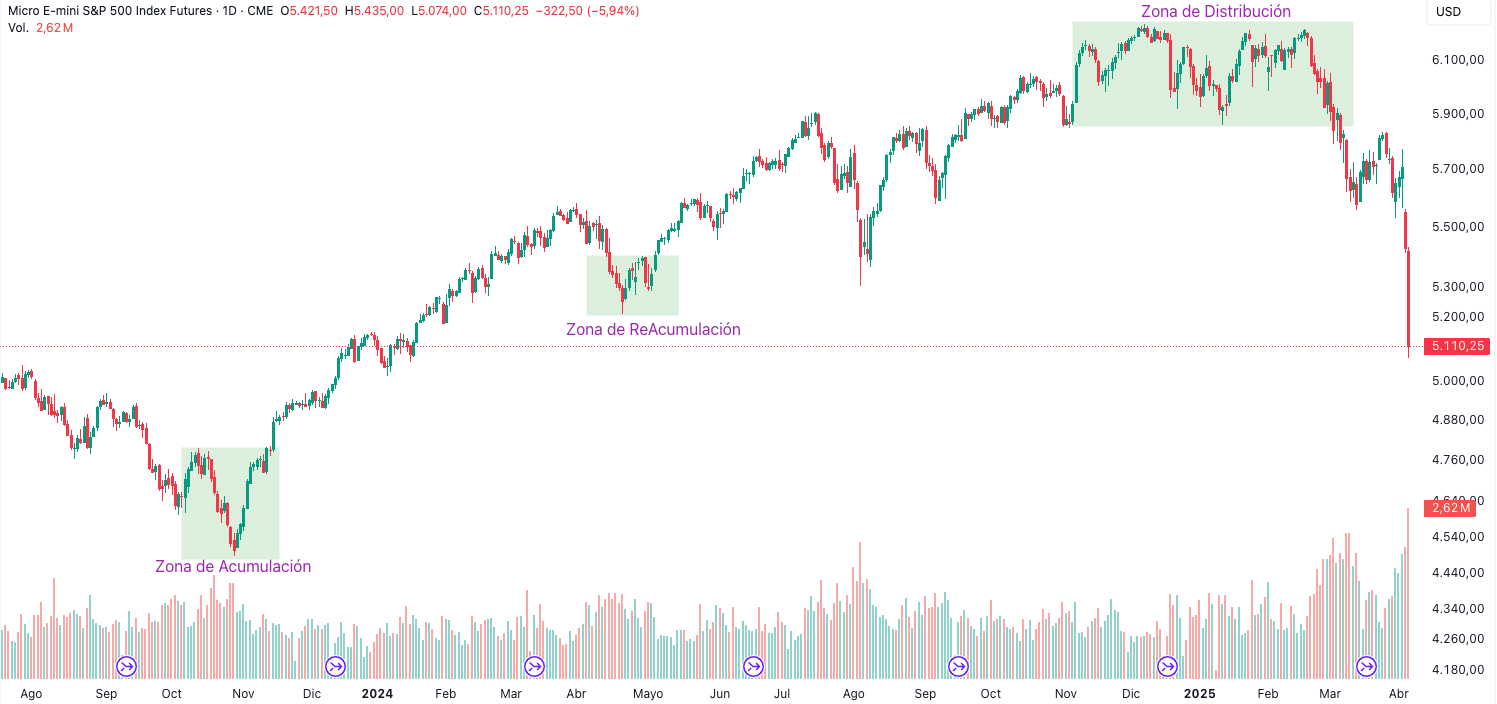
\includegraphics[width=11cm]{images/zonas_acumulacion_distribucion.png}
    \caption{Zonas de acumulaci\'on y distribuci\'on profesional en el MES-0625}
    \label{fig:zonas_acumulacion_distribucion}
\end{figure}
\vspace{0.5em}

\noindent
En la figura \ref{fig:zonas_acumulacion_distribucion} se ilustran dos zonas estructurales clave identificadas a partir del an\'alisis de \textbf{precio y volumen}, tal como lo propone \textbf{Miguel \'Angel Ram\'irez}, y que encuentran respaldo t\'acito en la lectura contextual de \textbf{Al Brooks}.

\begin{itemize}
    \item \textbf{Zona de Acumulaci\'on:} ubicada en la parte baja del gr\'afico, entre octubre de 2023 y noviembre de 2023. Se caracteriza por una fase lateral tras una ca\'ida prolongada, con velas de rango estrecho y volumen elevado, lo cual sugiere \textbf{absorci\'on profesional}. La salida alcista posterior, mediante velas de intenci\'on con volumen creciente, valida esta fase como acumulativa.

    \item \textbf{Zona de Distribuci\'on:} situada en el techo del mercado, entre noviembre de 2024 y febrero de 2025. Presenta un comportamiento lateral sin continuidad alcista, lo que indica \textbf{actividad vendedora encubierta}. La confirmaci\'on se da cuando el precio rompe los soportes internos del rango con una vela bajista de amplio rango y volumen extremo, iniciando una fase impulsiva descendente.

    \item \textbf{Principio de causa y efecto:} tal como sostiene Ram\'irez, \textbf{a mayor duraci\'on y volumen en estas zonas, mayor energ\'ia tendr\'a el movimiento posterior}. Este principio se observa en ambos casos, donde los desplazamientos posteriores fueron amplios y decididos.
\end{itemize}

\noindent
Estas zonas reflejan la participaci\'on activa del operador institucional y constituyen una herramienta de alta precisi\'on para anticipar transiciones estructurales en el mercado. Su correcta identificaci\'on permite actuar en sinton\'ia con la intenci\'on profesional y proyectar movimientos de alta probabilidad.



\subsection{Dilataciones y Falsas Rupturas}

Ambos autores coinciden en que las falsas rupturas (dilataciones) constituyen una herramienta estrat\'egica para los profesionales:

\begin{itemize}
    \item Las dilataciones se caracterizan por romper brevemente soportes o resistencias sin continuidad posterior, generando trampas que inducen al error a traders menos experimentados.
    
    \item Son reconocibles por el bajo volumen de ruptura, velas de rechazo inmediatas o por la falta de continuidad tras la vela inicial de ruptura.
    
    \item Detectar estas dilataciones tempranamente permite identificar los niveles verdaderos de acumulaci\'on o distribuci\'on profesional.
\end{itemize}


\subsection{Dilataciones y Falsas Rupturas}

Tanto Miguel \'Angel Ram\'irez como Al Brooks reconocen que las \textbf{dilataciones} o \textbf{falsas rupturas} son maniobras recurrentes del operador profesional para inducir a error al trader minorista y redistribuir la liquidez. Se trata de movimientos en apariencia decisivos que, al no presentar confirmaci\'on o continuidad posterior, revelan su naturaleza manipulativa.

\begin{itemize}
    \sloppy
    \item Las \textbf{dilataciones} ocurren cuando el precio rompe brevemente un soporte o resistencia relevante, para luego regresar r\'apidamente al rango anterior. Este comportamiento genera falsas se\~nales de ruptura que suelen \textbf{activar stops}, inducir entradas precipitadas y provocar reacciones emocionales en los operadores menos preparados.

    \item Ram\'irez describe estas maniobras como \textbf{trampas profesionales}, orientadas a \textbf{capturar liquidez} antes de realizar el movimiento verdadero. Estas rupturas se producen sin el respaldo de un volumen significativo ni de velas con intenci\'on clara, lo que las distingue de las rupturas aut\'enticas.

    \item Al Brooks, desde su perspectiva de acci\'on del precio pura, hace \'enfasis en que la ruptura de un nivel debe ser evaluada en funci\'on del \textbf{contexto previo} y la \textbf{reacci\'on inmediata posterior}. La falta de continuidad o la aparici\'on de una vela contraria fuerte suele ser indicio de una dilataci\'on.

    \item Los elementos t\'ecnicos que permiten identificar estas dilataciones incluyen:
    \begin{itemize}
        \item \textbf{Volumen bajo} en la ruptura o ruptura con volumen inusual pero sin continuidad.
        \item \textbf{Velas de rechazo inmediato}, con cuerpo estrecho y sombra larga en direcci\'on contraria.
        \item \textbf{Retorno r\'apido al rango} anterior o al canal previo.
    \end{itemize}

    \item Detectar estas maniobras permite al operador interpretar correctamente el \textbf{nivel real de inter\'es profesional} (acumulaci\'on o distribuci\'on), y aprovechar el enga\~no institucional como oportunidad operativa.
\end{itemize}

\noindent
En s\'intesis, las dilataciones no deben interpretarse como fallos del mercado, sino como \textbf{manifestaciones intencionadas del profesional}, cuyo objetivo es redistribuir posiciones, activar liquidez pasiva y \textbf{construir el movimiento real a contracorriente del consenso}. Reconocerlas a tiempo ofrece una ventaja decisiva en la lectura estructural del mercado.


\vspace{1em}
\noindent
\begin{figure}[!htbp]
    \centering
    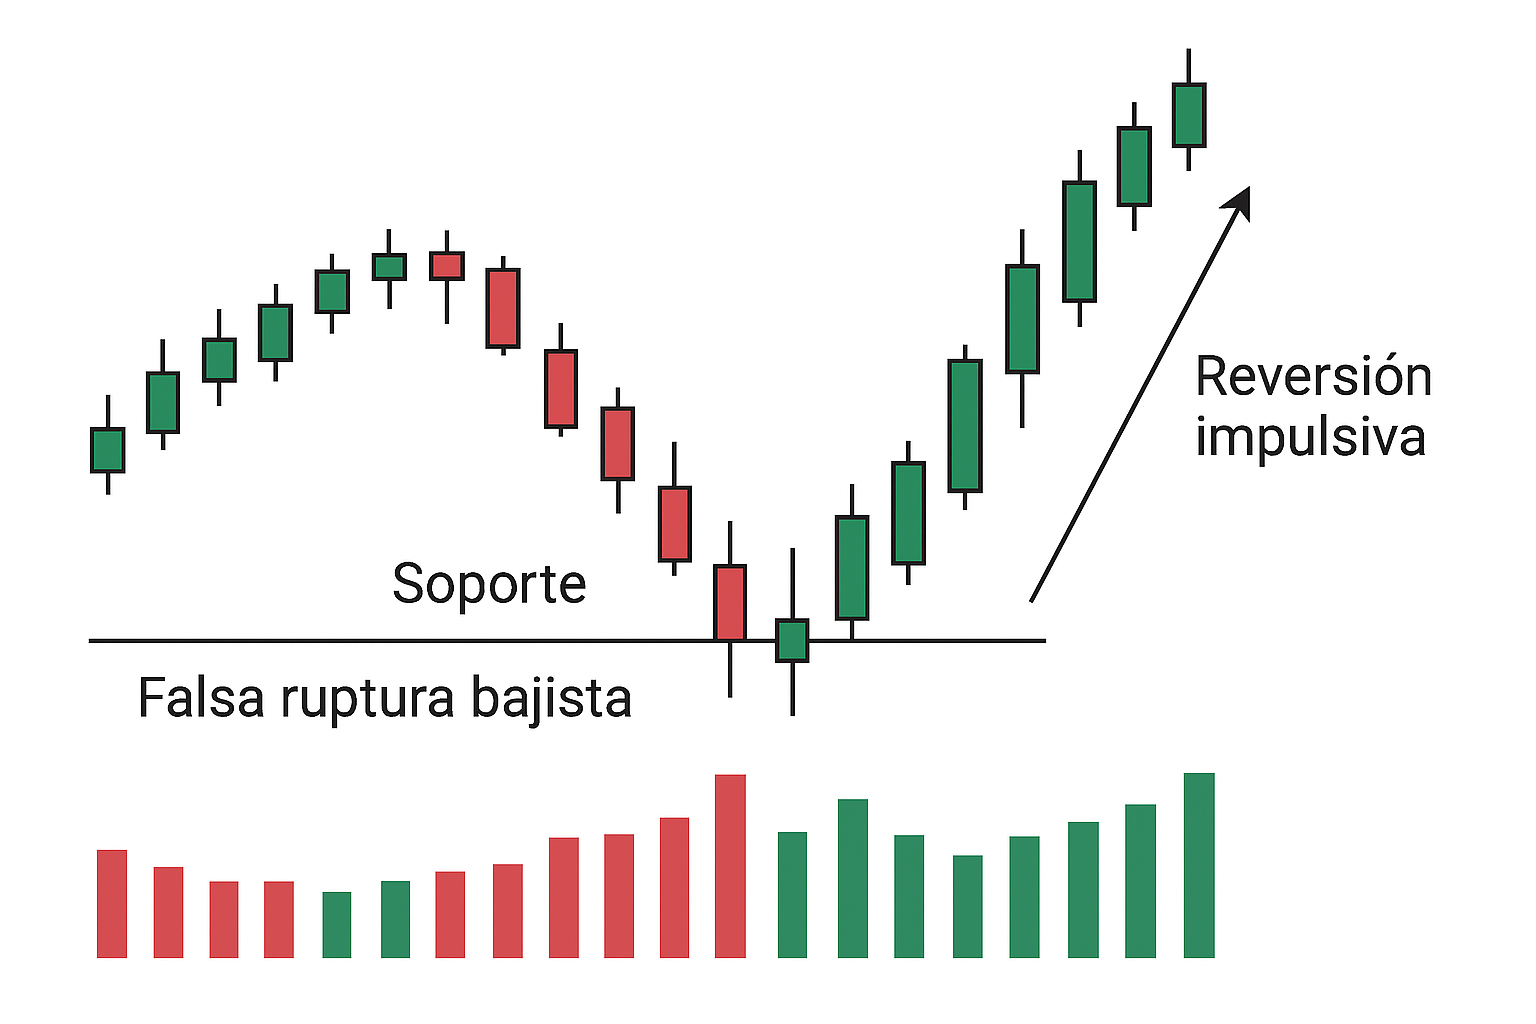
\includegraphics[width=11cm]{images/Dilatacion_Falsa_Ruptura.png}
    \caption{Falsa ruptura bajista seguida de reversi\'on impulsiva}
    \label{fig:Dilatacion_Falsa_Ruptura}
\end{figure}
\vspace{0.5em}

\noindent
En la figura \ref{fig:Dilatacion_Falsa_Ruptura} se ilustra un ejemplo cl\'asico de \textbf{dilataci\'on bajista}, tambi\'en denominada \textbf{falsa ruptura}, seguida por una \textbf{reversi\'on con intenci\'on}. Este tipo de estructura es descrita por \textbf{Miguel \'Angel Ram\'irez} como una maniobra de enga\~no profesional para capturar liquidez, y por \textbf{Al Brooks} como una ruptura fallida de un rango seguida de una entrada de segunda intenci\'on.

\begin{itemize}
    \item En la parte inferior del gr\'afico se destaca una \textbf{zona de soporte t\'ecnico}, la cual ha sido testeada previamente. Esta zona atrae atenci\'on por parte de operadores minoristas y algoritmos.

    \item La vela roja que rompe el soporte representa una \textbf{dilataci\'on}, caracterizada por su breve penetraci\'on del nivel sin continuidad posterior. El volumen es moderado o incluso bajo, y el precio no logra sostenerse por debajo del soporte.

    \item A continuaci\'on aparece una \textbf{vela verde de rechazo}, que anula la ruptura y confirma el fallo. Este es el punto de inflexi\'on que marca el \textbf{cambio de control institucional}.

    \item Lo que sigue es una \textbf{reversi\'on impulsiva}: varias velas alcistas consecutivas con cuerpo amplio, cierres en m\'aximos y volumen creciente. Esta secuencia confirma la intenci\'on institucional en direcci\'on contraria a la ruptura inicial.

    \item El patr\'on revela c\'omo el operador profesional induce al error a los traders menos experimentados, \textbf{absorbiendo su liquidez} antes de ejecutar el movimiento real.
\end{itemize}

\noindent
Este tipo de configuraci\'on es esencial dentro de la lectura institucional del mercado. Su correcta identificaci\'on permite al operador evitar trampas y alinearse con la verdadera intenci\'on del profesional, fortaleciendo la calidad de sus decisiones operativas.

\vspace{1em}
\noindent
\begin{figure}[!htbp]
    \centering
    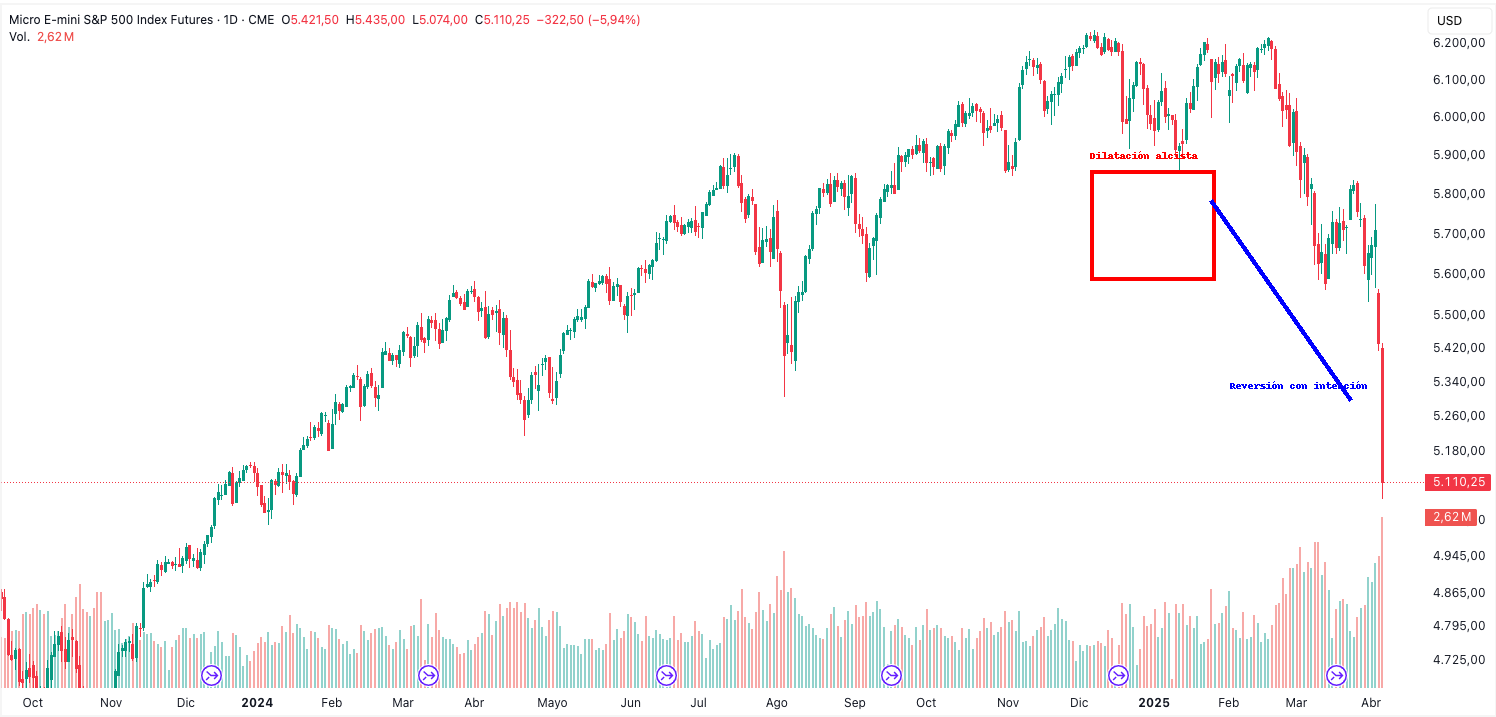
\includegraphics[width=11cm]{images/dilatacion_alcista_reversion.png}
    \caption{Dilataci\'on alcista en resistencia seguida de reversi\'on bajista con intenci\'on}
    \label{fig:dilatacion_alcista_reversion}
\end{figure}
\vspace{0.5em}

\noindent
La figura \ref{fig:dilatacion_alcista_reversion} muestra un caso representativo de \textbf{dilataci\'on alcista} o \textbf{falsa ruptura por encima de una resistencia relevante}, seguido por una \textbf{movilidad bajista con volumen e intenci\'on}, en el contrato MES-0625. Esta estructura es interpretada por \textbf{Miguel \'Angel Ram\'irez} como una trampa profesional orientada a inducir compras tard\'ias, y por \textbf{Al Brooks} como un fallo de ruptura que da paso a una entrada de segunda intenci\'on en sentido contrario.

\begin{itemize}
    \item La \textbf{zona roja} corresponde a una resistencia t\'ecnica previamente testeada por el precio. En dicha zona, el mercado rompe moment\'aneamente al alza, generando una aparente ruptura impulsiva que activa compras especulativas o stops de vendedores.

    \item Sin embargo, la ruptura carece de continuidad y es seguida por un \textbf{rechazo inmediato}, evidenciado en velas bajistas con volumen progresivamente mayor, lo que confirma la ausencia de convicci\'on institucional en la ruptura inicial.

    \item El movimiento posterior es una \textbf{reversi\'on bajista con intenci\'on}, en la que se suceden velas con cuerpo amplio, cierre en los extremos y volumen creciente. Esto valida el fallo como una maniobra de \textbf{distribuci\'on encubierta}.

    \item Esta dilataci\'on alcista permite redefinir el verdadero nivel de oferta institucional, y representa una oportunidad de entrada con ventaja informativa cuando se confirma el giro.
\end{itemize}

\noindent
Este tipo de secuencia es clave en la lectura profesional del mercado: permite identificar maniobras de manipulaci\'on por parte del operador institucional, y operar a favor del movimiento real con criterios de confirmaci\'on basados en \textbf{rechazo, volumen e intenci\'on}.


\subsection{Confirmaci\'on Operativa en Zonas Relevantes}

Para Brooks y Ram\'irez, la confirmaci\'on inmediata es clave para validar cualquier nivel relevante:

\begin{itemize}
    \item Una vela fuerte con volumen alto, seguida de continuidad en la direcci\'on de la ruptura, valida la zona relevante como punto de inflexi\'on genuino.
    
    \item La ausencia de continuidad posterior implica una falsa ruptura y ofrece una se\~nal operativa contraria, aprovechable por traders avanzados para incorporarse en sentido contrario al movimiento inicial enga\~noso.
\end{itemize}

\subsection{Integraci\'on Pr\'actica y Estrat\'egica}

Finalmente, una comprensi\'on profunda y operativa de estas zonas relevantes permite:

\begin{itemize}
    \item Detectar puntos cr\'iticos de entrada con riesgo controlado y alto potencial de recompensa.
    \item Reconocer tempranamente trampas profesionales y evitar posiciones desfavorables.
    \item Interpretar con claridad la intenci\'on profesional, tomando decisiones en consonancia con el verdadero flujo del mercado.
\end{itemize}

\subsection{Conclusi\'on sobre las Zonas Relevantes}

Las zonas relevantes, cuando se entienden profundamente desde el an\'alisis combinado del precio y volumen, ofrecen al operador una poderosa ventaja operativa. Ram\'irez y Brooks destacan la importancia de interpretar estas zonas desde la acci\'on real del mercado, reconociendo la intenci\'on profesional, validando las rupturas con volumen y buscando continuidad inmediata que confirme la fuerza real detr\'as de los movimientos. Este conocimiento profundo transforma la operativa en un ejercicio consciente y altamente efectivo, alineado con las fuerzas institucionales que realmente mueven los mercados.

\section{S\'intesis Operativa}

La combinaci\'on consciente de estos elementos convierte el trading en una pr\'actica profundamente profesional, alineada con las fuerzas institucionales dominantes, lo que aumenta significativamente las probabilidades de \'exito.

\begin{itemize}
    \item Identificaci\'on precisa de zonas relevantes.
    \item Confirmaci\'on de intenci\'on mediante testeo y secado.
    \item Interpretaci\'on de velas clave para entradas y salidas operativas.
    \item Gesti\'on estrat\'egica en contextos claramente definidos (dilataciones, recuperaciones, acumulaciones o distribuciones confirmadas).
\end{itemize}

``Encontrar la verdadera intenci\'on es la clave para poder actuar del lado correcto.''

\section*{Glosario t\'ecnico}

\vspace{1em}

\noindent A continuaci\'on se presenta un glosario operativo con las definiciones clave utilizadas en la estrategia, integrando terminolog\'ia de Ram\'irez, Brooks, Coulling y Neely:

\begin{description}[leftmargin=2cm, style=nextline]
    \item[Acumulaci\'on silenciosa:] Proceso de compras institucionales en una zona lateral con volumen bajo creciente y velas alcistas peque\~nas. Implica absorci\'on progresiva sin intenci\'on inmediata.
    
    \item[Distribuci\'on activa:] Zona de alto volumen con velas mixtas, donde grandes operadores venden posiciones en repuntes controlados. Suele finalizar con agotamiento.
    
    \item[Volumen de intenci\'on:] Volumen que excede el 2.5x del promedio en velas de rango medio-alto. Indica presencia institucional clara (Ram\'irez).
    
    \item[Stopping volume:] Pico de volumen en vela con sombra inferior prolongada y cierre en mitad o parte superior. Implica freno de ca\'ida y posible giro (Coulling).
    
    \item[Reversi\'on por pin bar:] Vela con mecha larga (superior o inferior), cuerpo peque\~no y volumen menor al promedio. Detecta trampas y rechazo institucional (Brooks).
    
    \item[Correcci\'on plana:] Estructura de 3 ondas ABC donde B sobrepasa el inicio de A y C no logra superar a A. Detecta consolidaci\'on inestable (Neely).
    
    \item[Zigzag correctivo:] Patr\'on impulsivo correctivo en 3 tramos (A–B–C) con retrocesos claros. Cierra estructura r\'apida de correcci\'on (Neely).
    
    \item[Divergencia volumen–precio:] Desfase entre aumento/disminuci\'on de precio sin confirmaci\'on del volumen. Se interpreta como se\~nal de agotamiento o trampa.
    
    \item[Canal alcista moderado:] Serie de m\'inimos y m\'aximos ascendentes con volumen constante o decreciente. Indica continuidad profesional sin euforia.
    
    \item[Rango estrecho:] Zona lateral con velas peque\~nas y volumen bajo. Suele preceder a movimiento brusco si hay absorci\'on acumulativa.
    
    \item[Trampa de ruptura:] Movimiento repentino fuera del rango con bajo volumen, seguido de retorno r\'apido. Indica enga\~no de mercado.
    
    \item[Testeo profesional:] Vela peque\~na tras un rally, con volumen bajo y sin seguimiento. Confirma absorci\'on o distribuci\'on previa.
    
    \item[Breakout v\'alido:] Ruptura con vela de cuerpo completo, volumen superior a 2.5x el promedio y sin mecha contraria dominante.
    
    \item[Backtest de nivel:] Regreso al nivel recientemente roto, con vela de rango medio y volumen decreciente. Valida continuidad.
    
    \item[Media direccional de 15m:] Media m\'ovil simple de 10 velas en marco de 15 minutos. Define sesgo institucional para filtrar entradas.
    
    \item[Engulfing decisivo:] Vela envolvente con cuerpo grande, que cubre al menos dos velas previas, con volumen 2x superior. Se\~nal fuerte de giro (Brooks).
\end{description}

\vspace{2em}

\subsection*{Ejemplos operativos por concepto}

A continuaci\'on se presentan ejemplos t\'ipicos de aplicaci\'on contextual en entorno real (nivel 5800, ES-0625):

\begin{itemize}
    \item \textbf{Acumulaci\'on silenciosa:} Zona entre 5790–5800 con velas alcistas peque\~nas y volumen estable (1800–2200 contratos), sin ruptura inmediata.
    
    \item \textbf{Stopping volume:} Vela con sombra inferior larga en 5788, cuerpo pequeño, volumen 5000 contratos; cierra en 5791. Implica absorci\'on institucional.
    
    \item \textbf{Trampa de ruptura:} Ruptura bajista de 5785 con volumen de 1000 contratos; siguiente vela engulfing alcista con 3500 contratos. Falsa ruptura detectada.
    
    \item \textbf{Correcci\'on plana irregular:} Estructura A: 5810–5790, B: 5790–5815, C: 5815–5805. Volumen decreciente en C y stopping volume en 5805.
\end{itemize}

\vspace{2em}

\subsection*{Ruido y trampas: detecci\'on y filtros operativos}

En marcos de 2 minutos, el ruido puede inducir entradas falsas o anticipadas. Para mitigar su impacto, se emplean los siguientes filtros:

\begin{itemize}
    \item \textbf{Filtro correctivo:} No operar dentro de estructuras correctivas activas (zigzag o plana) hasta confirmaci\'on de onda C con volumen e intenci\'on clara.

    \item \textbf{Filtro de divergencia:} Si el precio sube y el volumen decrece, evitar entradas alcistas. Confirmar con vela de agotamiento o rechazo (Coulling).

    \item \textbf{Filtro de validaci\'on institucional:} Si el volumen no alcanza el umbral din\'amico (2.2x media de 10 velas), no asumir ruptura ni continuidad.

    \item \textbf{Filtro de contexto multinivel:} Si la media de 15 minutos est\'a plana o en contra, abstenerse de operar. Esperar alineaci\'on.

    \item \textbf{Se\~nales de trampa comunes:}
    \begin{itemize}
        \item Vela pin bar con volumen bajo.
        \item Vela con cuerpo largo sin volumen.
        \item Doji tras vela impulsiva sin continuidad.
        \item Rango estrecho con volumen creciente.
    \end{itemize}
\end{itemize}

\chapter{Pautas Correctivas}  % Conceptos relativos a la operativa

El mercado alterna entre \textbf{impulsos} (movimientos en la direcci\'on de la tendencia) y \textbf{correcciones} (retrocesos opuestos). Las \textbf{pautas correctivas} permiten identificar estos retrocesos, anticipar su fin y optimizar entradas en la tendencia, respetando un \textit{l\'imite correctivo} que, si se supera, indica una nueva tendencia. Este cap\'itulo aborda su definici\'on, clasificaci\'on y aplicaci\'on pr\'actica, integrando enfoques de Elliott, Neely, Coulling, Ram\'irez y Prechter para traders del S\&P 500 (ES), especialmente en marcos de 2 minutos.

Las pautas correctivas son clave para mapear escenarios de precios y determinar la fase del ciclo del mercado. Adem\'as, representan procesos de \textit{acumulaci\'on-reacumulaci\'on} y/o \textit{distribuci\'on-redistribuci\'on}~\cite{ramirez18}.

\section{Concepto y Caracter\'isticas}

Estas pautas suelen estar compuestas por tres segmentos principales, etiquetados generalmente como A-B-C. Permiten anticipar pausas en la tendencia y valorar una posible continuaci\'on o reversi\'on. A diferencia de las ondas impulsivas, suelen ser m\'as complejas y menos evidentes, con patrones que requieren interpretaci\'on cuidadosa del volumen y del comportamiento del precio.

\textbf{En s\'intesis:}
\begin{itemize}
    \item Tras un impulso (e.g., subida de 100 puntos), se espera otro impulso en la misma direcci\'on.
    \item Entre impulsos, se identifica una pauta correctiva (e.g., retroceso de 38-50 puntos).
    \item Una correcci\'on no debe igualar ni superar el rango del impulso previo.
    \item Retrocesos muy peque\~nos (5-10 puntos) son pausas, no correcciones significativas.
\end{itemize}

\section{Clasificaci\'on de las Pautas Correctivas}

\subsection{Pautas Correctivas Simples}

\subsubsection{MonoOnda}
Una \textbf{MonoOnda} es un movimiento continuo, generalmente recto, con pausas menores (<20\%) pero sin tramos correctivos definidos (A-B-C). Es com\'un en onda 2 y marca el inicio o fin de una correcci\'on mayor~\cite{Neely04}.

\begin{figure}[!htbp]
    \centering
    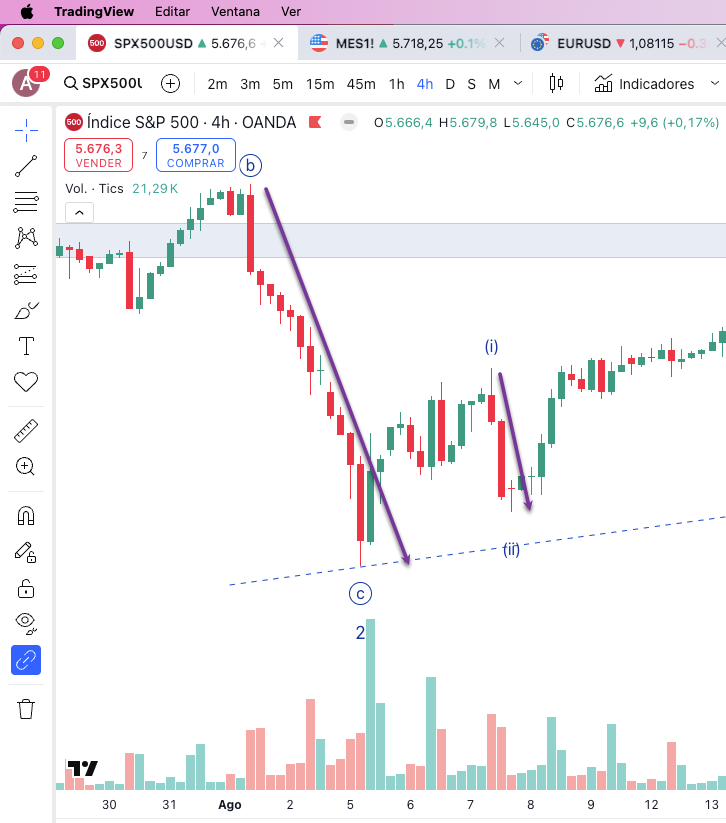
\includegraphics[width=10cm]{images/Pauta_Monoonda.png}
    \caption{Pauta MonoOnda}
    \label{fig:Pauta_Monoonda}
\end{figure}

En la figura \ref{fig:Pauta_Monoonda} se observa ejemplo de MonoOnda en marco de 4 horas. Desde el punto \textbf{b} hasta el punto \textbf{C}, se observa un movimiento bajista continuo, sin retrocesos significativos y con estructura directa, lo cual es característico de una pauta \textbf{MonoOnda}. Esta estructura coincide con una onda 2, validada además por el incremento notorio de volumen en el final del tramo, indicando absorción institucional y posible cambio de fase.

\subsubsection{Pautas ABC~\cite{Elliottwave}}
Estas correcciones de tres segmentos incluyen dos ondas impulsivas (A y C) con cinco subondas, y una onda correctiva (B) con tres subondas, conocida como ``el ni\~no tonto'' por su imprevisibilidad.

\paragraph{Zig-Zag Normal}
Patr\'on 5-3-5. En la figura \ref{fig:ZigZag}, tras un impulso a 100, A cae a 70, B sube a 85, y C baja a 55.

\begin{figure}[!htbp]
    \centering
    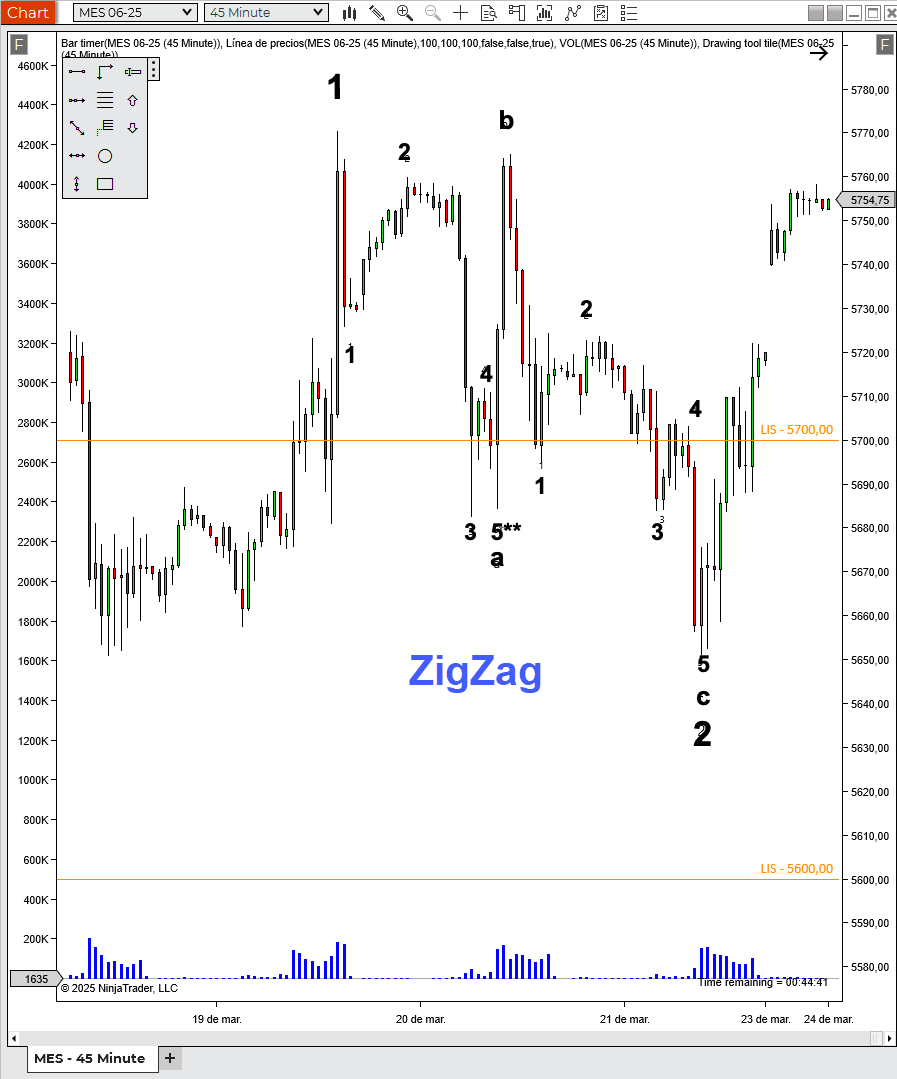
\includegraphics[width=10cm]{images/ZigZag.png}
    \caption{Pauta ABC: Zig-Zag}
    \label{fig:ZigZag}
\end{figure}

En la figura \ref{fig:ZigZag} se visualiza el ejemplo de Zig-Zag en gráfico de 45 minutos. El precio forma una pauta 5-3-5 claramente identificable: la onda \textbf{a} presenta cinco subondas descendentes, seguida por una onda \textbf{b} correctiva de tres segmentos, y finalmente una onda \textbf{c} con cinco subondas adicionales. La estructura cumple con los requisitos clásicos del Zig-Zag según la Teoría de Elliott, y marca la onda 2 de una estructura mayor.

\paragraph{Plana Normal~\cite{Elliottwave,ramirez18}}
Patr\'on 3-3-5. B se acerca al inicio de A, y C baja ligeramente por debajo de A.

\begin{figure}[!htbp]
    \centering
    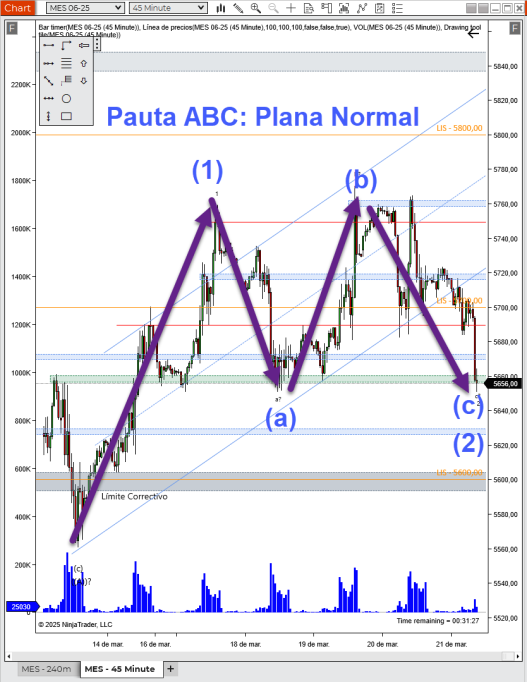
\includegraphics[width=9cm]{images/Pauta_ABC_Plana_Normal.png}
    \caption{Pauta ABC: Plana Normal}
    \label{fig:Pauta_ABC_Plana_Normal}
\end{figure}

La figura \ref{fig:Pauta_ABC_Plana_Normal} muestra un ejemplo de pauta ABC tipo Plana Normal en gráfico de 45 minutos. Se observa una estructura de tres ondas: \textbf{a} y \textbf{b} compuestas por tres subondas cada una, y \textbf{c} con cinco subondas. La onda \textbf{b} retrocede casi completamente el recorrido de la onda \textbf{a}, sin superarlo, y la onda \textbf{c} se extiende ligeramente por debajo del final de la onda \textbf{a}. Esta configuración respeta la simetría del patrón 3-3-5 típico de las planas normales, y señala el final de una corrección clasificada como onda (2).

\paragraph{Plana Irregular o Fallo Irregular}
La onda B supera el inicio de A y C no alcanza el final de A, indicando un fallo. 

\begin{itemize}
    \item \textbf{Neely}: B excede el 61.8\% del rango de A, y C es m\'as corta.
    \item \textbf{Ram\'irez}: B refleja un intento fallido institucional.
    \item \textbf{Coulling}: Alto volumen en B y bajo en C indica agotamiento.
\end{itemize}

\begin{figure}[!htbp]
    \centering
    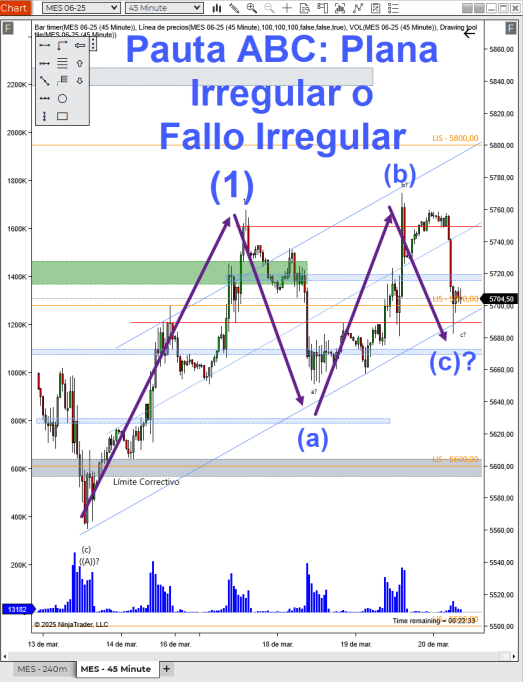
\includegraphics[width=9cm]{images/Pauta_ABC_Plana_Irregular.png}
    \caption{Pauta ABC: Plana Irregular}
    \label{fig:Pauta_ABC_Plana_Irregular}
\end{figure}

En la figura \ref{fig:Pauta_ABC_Plana_Irregular} se presenta el ejemplo de pauta ABC tipo Plana Irregular en gráfico de 45 minutos. La onda \textbf{b} excede con claridad el inicio de la onda \textbf{a}, lo que indica un exceso de entusiasmo comprador, en línea con la regla de Neely que exige un retroceso mayor al 61.8\% del rango de \textbf{a}. La onda \textbf{c}, por su parte, no logra superar el mínimo de la onda \textbf{a}, generando un fallo. Este patrón sugiere agotamiento institucional, especialmente si se confirma con un alto volumen en \textbf{b} y bajo en \textbf{c}, como propone Coulling. Ramírez interpreta esta estructura como un intento institucional fallido de sostener la tendencia previa.

\subsection{Pautas Correctivas Complejas}

\paragraph{Double y Triple Combinations~\cite{Elliottwave}}
Dos o tres patrones correctivos conectados por una o dos X-waves.

Las \textbf{combinaciones dobles y triples} son estructuras correctivas complejas que, seg\'un la teor\'ia de la Onda de Elliott (y ampliadas por Neely y Prechter), se componen de dos o tres patrones correctivos simples conectados por una o dos ondas \textbf{X}. Su objetivo es extender la correcci\'on en el tiempo, sin alterar significativamente el precio, generando estructuras laterales dif\'iciles de interpretar para el operador promedio.

\begin{itemize}
    \item \textbf{Double Combination (W--X--Y):} consiste en dos patrones correctivos (W y Y) conectados por una onda X. Los patrones m\'as comunes que la conforman son:
    \begin{itemize}
        \item Zigzag + Plano
        \item Zigzag + Tri\'angulo
        \item Plano + Tri\'angulo
    \end{itemize}
    La onda X suele ser menos profunda y m\'as compleja que un simple retroceso.

    \item \textbf{Triple Combination (W--X--Y--X--Z):} extiende a\'un m\'as la correcci\'on agregando una tercera estructura (Z), conectada por una segunda onda X. Este patr\'on refleja una clara intenci\'on del mercado de \textbf{consumir tiempo sin avanzar}, formando una consolidaci\'on amplia, muchas veces en forma de canal horizontal.

    \item \textbf{Rasgos comunes:}
    \begin{itemize}
        \item Predominan en ondas 4 o correcciones complejas de onda B.
        \item Las estructuras internas deben estar bien definidas, aunque pueden alternar en forma.
        \item El volumen tiende a disminuir progresivamente, y la acci\'on del precio se vuelve m\'as err\'atica a medida que la pauta se desarrolla.
    \end{itemize}
\end{itemize}

\begin{figure}[!htbp]
    \centering
    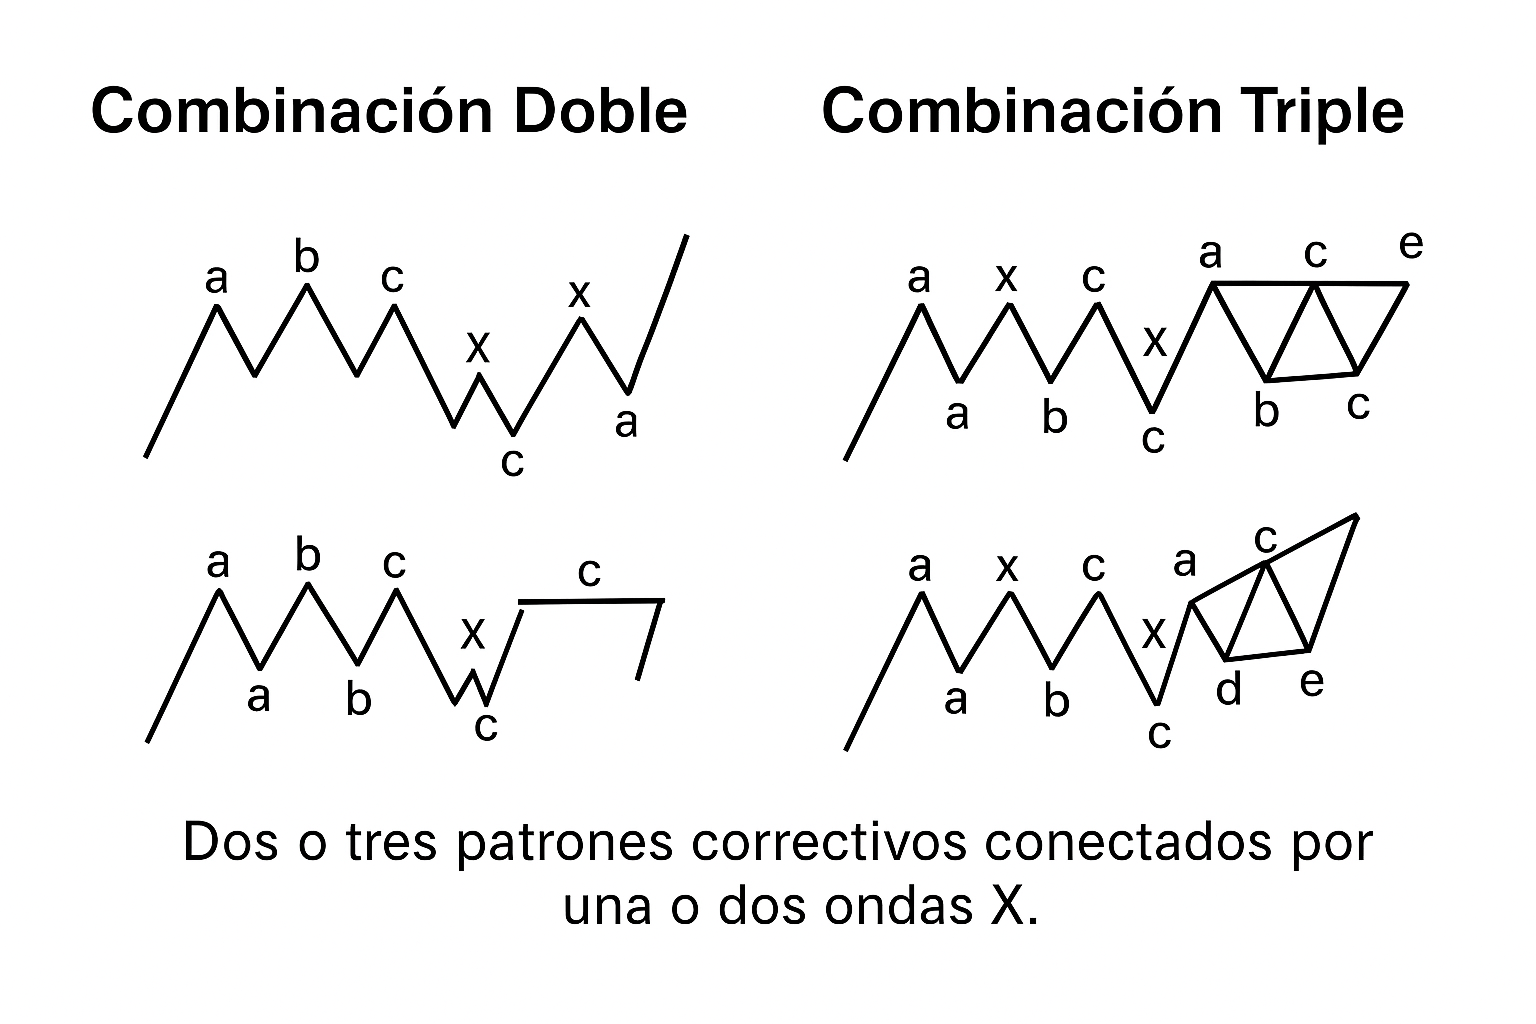
\includegraphics[width=9cm]{images/Dobles_Triples_Combinaciones.png}
    \caption{Dobles y Triples Combinaciones}
    \label{fig:Dobles_Triples_Combinaciones}
\end{figure}

En la figura \ref{fig:Dobles_Triples_Combinaciones} se presenta el esquema visual de las pautas Double (W--X--Y) y Triple Combination (W--X--Y--X--Z)

\noindent
Comprender estas combinaciones permite al analista anticipar una mayor complejidad estructural cuando las correcciones simples fallan, y facilita mantenerse fuera del mercado hasta que se rompa claramente la estructura lateral. Su identificaci\'on es clave para evitar entradas impulsivas durante fases correctivas extendidas.

\begin{figure}[!htbp]
    \centering
    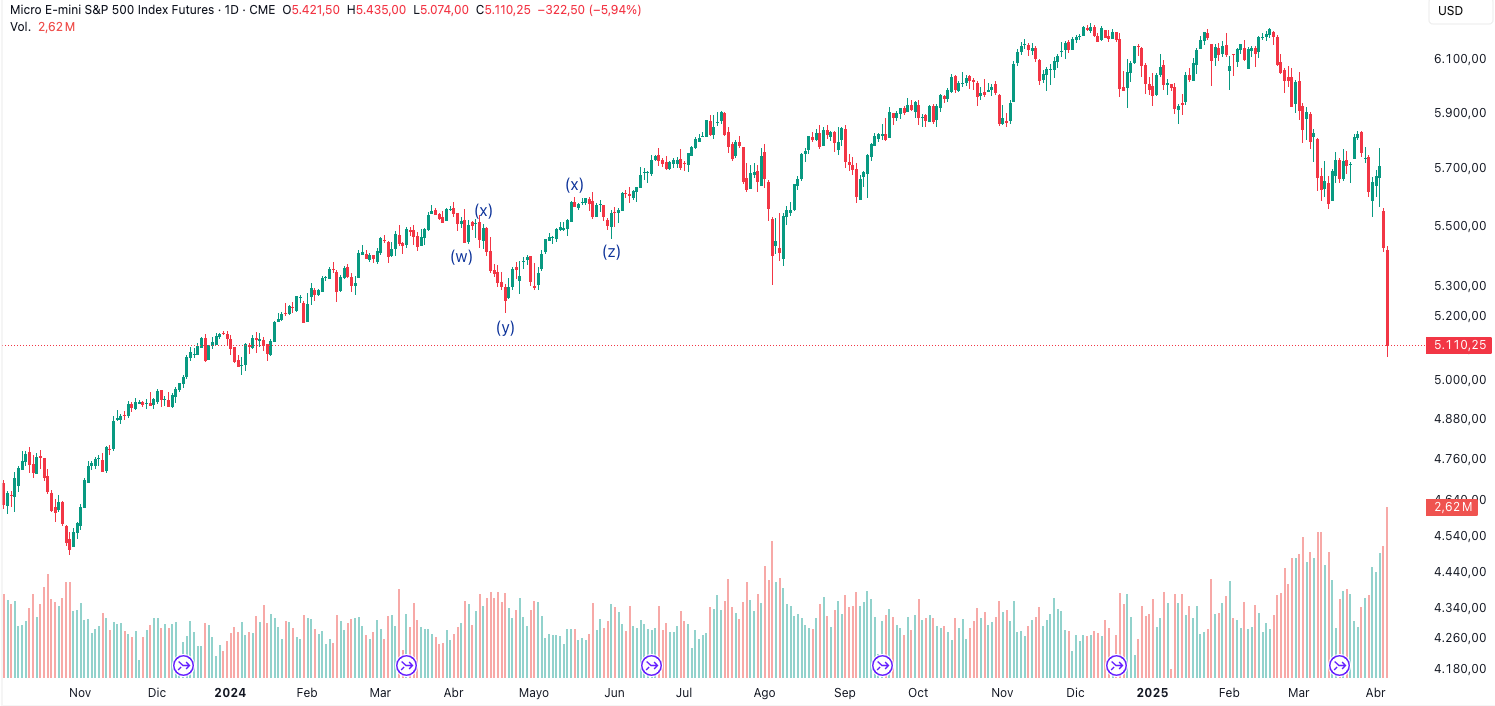
\includegraphics[width=9cm]{images/double_triple_combination_mes0625.png}
    \caption{Pauta Triple Combination (w)--(x)--(y)--(x)--(z) en el MES-0625}
    \label{fig:double_triple_combination_mes0625}
\end{figure}

\noindent
Estas estructuras, descritas por Elliott y expandidas por Neely, tienen como funci\'on principal \textbf{consumir tiempo sin generar desplazamiento significativo}, frustrando tanto a compradores como a vendedores. Su identificaci\'on temprana permite evitar entradas impulsivas y anticipar el momento de ruptura real.

\noindent
En la figura \ref{fig:double_triple_combination_mes0625} se presenta una estructura correctiva del tipo \textbf{Triple Combination}, etiquetada como \textbf{(w)--(x)--(y)--(x)--(z)}, desarrollada durante el a\~no 2024 en el contrato \textbf{MES-0625}. Este tipo de pauta pertenece a las \textbf{correcciones complejas} descritas en la teor\'ia de la Onda de Elliott y ampliadas por autores como Glenn Neely, y se caracteriza por combinar tres patrones correctivos simples mediante dos ondas conectivas (\textbf{x}).
La figura \ref{fig:double_triple_combination_mes0625} muestra un ejemplo operativo de una \textbf{pauta correctiva compleja del tipo Triple Combination} en el contrato \textbf{MES-0625}, desarrollado entre los meses de \textbf{enero y septiembre de 2024}. Esta estructura lateral se inscribe dentro de una fase de distribuci\'on institucional y se caracteriza por encadenar tres patrones correctivos (\textbf{W}, \textbf{Y} y \textbf{Z}) conectados por dos ondas \textbf{X}.


\begin{itemize}
    \item \textbf{(w):} Primera fase correctiva que da inicio a la consolidaci\'on. Suele adoptar la forma de un \textbf{zigzag} o un \textbf{plano} r\'apido. La primera estructura correctiva, usualmente un zigzag o un plano, representa el primer intento del mercado por corregir la tendencia previa.   
    \item \textbf{(x):} Onda conectiva que introduce una pausa o retroceso, extendiendo la duraci\'on sin cambiar significativamente la direcci\'on general del mercado. Conecta la estructura W con Y. Puede ser un retroceso parcial o una figura propia como un tri\'angulo o un canal.
    \item \textbf{(y):} Segunda pauta correctiva, diferente en estructura a (w), que mantiene la l\'ogica de lateralidad y aumenta la complejidad del patr\'on. Segunda estructura correctiva, que puede diferir en forma respecto a W (principio de alternancia). En el ejemplo, mantiene la l\'ogica de consolidaci\'on sin generar desplazamiento impulsivo.
    \item \textbf{(x):} Segunda onda de conexi\'on, generalmente de menor amplitud y m\'as err\'atica que la primera. Su funci\'on es preparar el terreno para el tramo final de la correcci\'on. Conecta el segundo bloque con la estructura final. Su comportamiento err\'atico refuerza la naturaleza no direccional de la pauta.
    \item \textbf{(z):} Tercera y \'ultima pauta correctiva, que concluye la formaci\'on de la combinaci\'on triple. Esta parte suele ser la m\'as dif\'icil de anticipar, ya que agota la fase correctiva sin se\~nales direccionales claras. La tercera y \'ultima estructura correctiva. Culmina el patr\'on extendiendo la duraci\'on de la consolidaci\'on y preparando el terreno para un eventual movimiento impulsivo posterior.
\end{itemize}

\noindent
Este patr\'on refleja la intenci\'on del mercado de \textbf{consumir tiempo sin generar desplazamiento neto}, lo que produce frustraci\'on en operadores que buscan continuidad direccional. Su correcta identificaci\'on es fundamental para evitar entradas err\'aticas durante fases de consolidaci\'on y anticipar rupturas significativas posteriores, como la que se observa al final de la pauta (z), donde el precio rompe a la baja con volumen e intenci\'on.


\paragraph{Diametric y Symmetrical~\cite{Neely04}}

Dentro del enfoque de \textbf{Glenn Neely}, los patrones \textbf{Diametric} y \textbf{Symmetrical} representan estructuras correctivas altamente complejas, compuestas por \textbf{siete subondas sim\'etricas}, etiquetadas como \textbf{A--B--C--D--E--F--G}. Son comunes en \textbf{consolidaciones laterales prolongadas} y se caracterizan por su notable equilibrio geom\'etrico y temporal.

\begin{itemize}
    \item Cada subonda cumple una funci\'on correctiva; ninguna de ellas es impulsiva. El patr\'on alterna la direccionalidad de forma equilibrada, dando lugar a un movimiento contenido y arm\'onico dentro de un rango definido.
    \item La \textbf{simetr\'ia} se expresa mediante la relaci\'on entre ondas opuestas: A se corresponde con G, B con F y C con E, mientras que la onda D act\'ua como eje central estructural y temporal. Esta disposici\'on genera un patr\'on visual de tipo ``diamante''.
    \item Seg\'un Neely, estas formaciones reflejan un \textbf{proceso de transici\'on neutra}, en el que el mercado consume tiempo sin generar desplazamiento neto significativo, muchas veces prepar\'andose para una fase impulsiva posterior.
    \item Aunque el patr\'on tiene naturaleza lateral, puede adoptar una leve inclinaci\'on ascendente o descendente, sin perder su car\'acter de consolidaci\'on estructurada.
    \item Para que un \textit{diametric} sea v\'alido, debe completarse \'integramente la secuencia de siete ondas antes de cualquier ruptura decisiva del rango. La onda G debe concluir en una zona de definici\'on direccional clara, muchas veces acompa\~nada de volumen e intenci\'on.
\end{itemize}

\noindent
Este tipo de estructuras puede confundirse con tri\'angulos, canales o combinaciones triples. No obstante, se distingue por su n\'umero exacto de fases, su \textbf{simetr\'ia interna}, y por obedecer a principios estrictos de \textbf{alternancia, proporci\'on y equilibrio temporal}. Su correcta identificaci\'on permite anticipar el fin de fases de congesti\'on y prepararse para movimientos de alta direccionalidad.


\begin{figure}[!htbp]
    \centering
    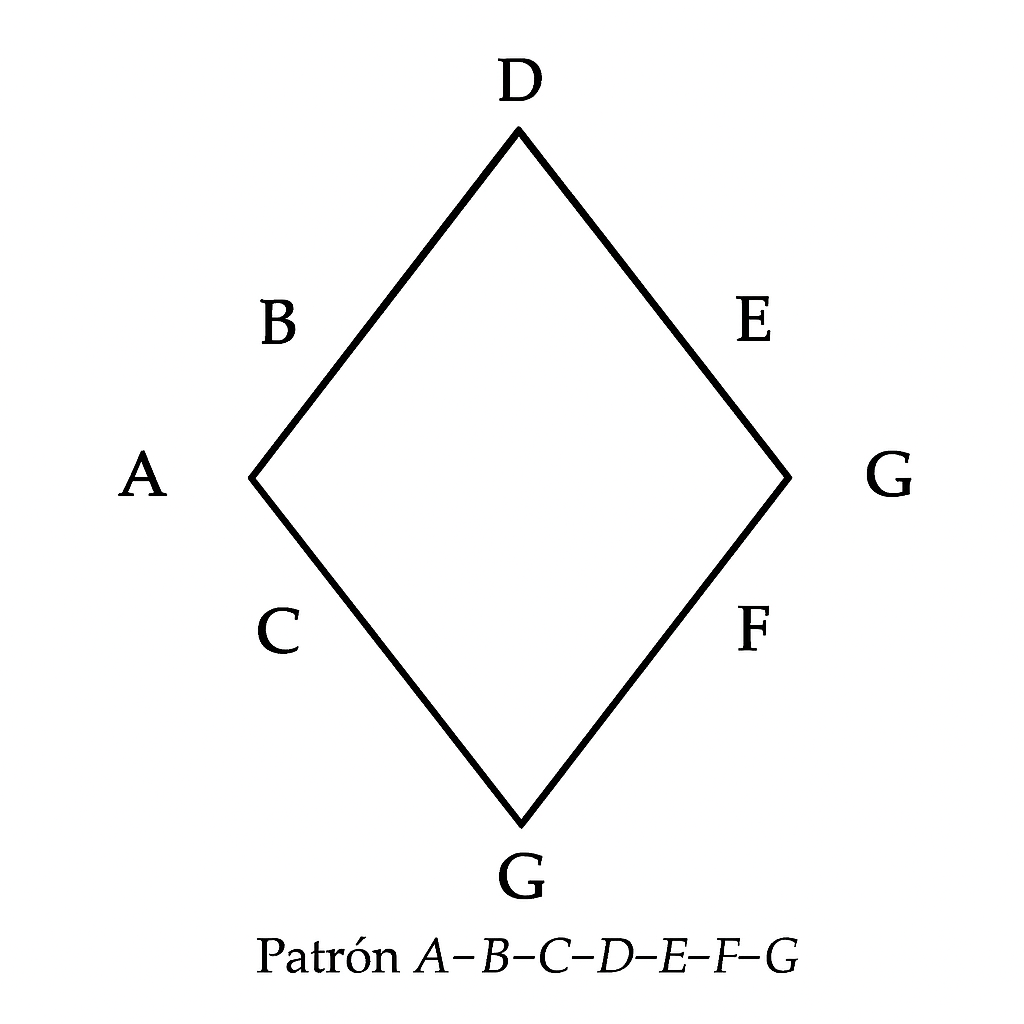
\includegraphics[width=11cm]{images/digital_diagram_features_a_sy.png}
    \caption{Esquema did\'actico del patr\'on sim\'etrico tipo \textit{Diametric} (A--B--C--D--E--F--G)}
    \label{fig:digital_diagram_features_a_sy}
\end{figure}

\vspace{1em}

\noindent
La imagen \ref{fig:digital_diagram_features_a_sy} representa un \textbf{patr\'on correctivo complejo sim\'etrico}, clasificado por Glenn Neely como un \textbf{Diametric} o \textbf{Symmetrical}, compuesto por \textbf{siete subondas} etiquetadas como \textbf{A--B--C--D--E--F--G}. Este patr\'on se caracteriza por su disposici\'on equilibrada y por emerger en contextos de \textbf{consolidaci\'on lateral prolongada}, donde el mercado consume tiempo sin avanzar significativamente.

\begin{itemize}
    \item La estructura est\'a organizada en torno a un eje central (onda D), a partir del cual se reflejan las subondas en sentido sim\'etrico: A se corresponde con G, B con F, y C con E.    
    \item Cada subonda tiene car\'acter correctivo, sin mostrar intenci\'on ni volumen suficiente para establecer una direccionalidad sostenida. Esto produce un patr\'on visual tipo ``diamante'' que puede tener inclinaci\'on ascendente, descendente o completamente horizontal.    
    \item El patr\'on es frecuente en fases de transici\'on, particularmente como onda B o como parte de una correcci\'on interna dentro de estructuras m\'as amplias. Su reconocimiento temprano permite al analista evitar operaciones en entornos de baja probabilidad y prepararse para la ruptura posterior.    
    \item La onda G suele ser la clave operativa, pues su ruptura puede activar el siguiente tramo impulsivo. Sin embargo, esta debe ir acompa\~nada de \textbf{volumen, intenci\'on y ruptura clara de la estructura sim\'etrica}.
\end{itemize}

\noindent
Este esquema permite identificar el patr\'on en su forma pura y sirve como referencia para comparar con estructuras reales observadas en el gr\'afico. Su utilidad reside en detectar fases de agotamiento estructural o pausa institucional dentro del ciclo de Elliott-Neely.

%\begin{figure}[H]
%    \centering
%    \includegraphics[width=\textwidth]{patron_diametric_mes0625.png}
%    \caption{Identificaci\'on de un patr\'on Diametric (A--B--C--D--E--F--G) en el MES-0625}
%\end{figure}

\textbf{Pendiente de Buscar y Encontrar el patrón para adicionarlo como imagen. El que encontré no me gustó mucho}

\vspace{1em}

\noindent
En esta figura se ha identificado una posible estructura \textbf{Diametric} dentro del contrato \textbf{MES-0625}, comprendida entre los meses de \textbf{diciembre de 2023 y agosto de 2024}. Este patr\'on correctivo complejo, descrito por \textbf{Glenn Neely}, se compone de \textbf{siete subondas correctivas} dispuestas de manera \textbf{sim\'etrica} y alternante: \textbf{A--B--C--D--E--F--G}.

\begin{itemize}
    \item La onda central \textbf{D} act\'ua como \textbf{eje estructural y temporal}, dividiendo el patr\'on en dos mitades que reflejan simetr\'ia tanto en duraci\'on como en amplitud.
    \item Las ondas \textbf{A--B--C} presentan una inclinaci\'on bajista suave, mientras que \textbf{E--F--G} replican dicha estructura en sentido contrario, con una inclinaci\'on ascendente leve. Este equilibrio genera una figura de tipo ``diamante'' caracter\'istica.
    \item El patr\'on se desarrolla en una fase de \textbf{consolidaci\'on lateral}, sin que exista desplazamiento neto claro. La \textbf{falta de intenci\'on} durante su formaci\'on sugiere acumulaci\'on de energ\'ia por parte del operador institucional.
    \item Este tipo de formaciones, seg\'un Neely, act\'uan como \textbf{pausas estructuradas} dentro del ciclo mayor y su resoluci\'on suele preceder un movimiento direccional importante. En este caso, la ruptura bajista posterior valida la hip\'otesis correctiva previa.
\end{itemize}

\noindent
La lectura correcta de este tipo de patrones permite anticipar el final de fases de congesti\'on y proyectar la direccionalidad subsecuente. Es fundamental observar la \textbf{estructura interna, la simetr\'ia relativa} y la \textbf{ruptura final con volumen} como confirmaci\'on operativa.



\section{Identificaci\'on en Tiempo Real}

En marcos de 2 minutos, detectar el fin de una pauta es vital. Se priorizan patrones de velas (e.g., engulfing), rompimientos de l\'ineas de tendencia (Brooks), y \textit{stopping volume} (Coulling).

\section{Enfoques Complementarios}

\subsection{Anna Coulling: Volumen y Precio}
El \textit{stopping volume} y la debilidad en rallies permiten confirmar o descartar pautas. Es clave en zonas de onda B o C.

\subsection{Glenn Neely: Precisi\'on con NEoWave}
Aplica proporciones Fibonacci y patrones como \textit{diametrics}. C debe ser 61.8\% de A y durar 1.618 veces su tiempo.

\subsection{Robert Prechter: Relaciones Fibonacci}
El uso de proporciones permite ubicar soportes y resistencias para prever puntos de reversi\'on.

\subsection{Miguel \'Angel Ram\'irez: Psicolog\'ia del Mercado}
Las correcciones reflejan estados emocionales colectivos: miedo, duda o agotamiento.

\subsection{Al Brooks: Patrones de Precio}
Proporciona confirmaci\'on adicional con patrones de velas (dobles techos, suelos, barras internas).

\section{Errores Comunes y C\'omo Evitarlos}

\begin{itemize}
    \item Confundir pausas con correcciones: validar con volumen.
    \item Malinterpretar la onda B: requiere paciencia y confirmaci\'on.
    \item Ignorar el l\'imite correctivo: si se rompe, se invalida el impulso anterior.
\end{itemize}

\section{Conclusi\'on}

Las pautas correctivas, desde simples (MonoOnda, ABC) hasta complejas (Diametric), combinan estructura t\'ecnica (Elliott, Neely, Prechter), volumen (Coulling), psicolog\'ia de mercado (Ram\'irez) y acci\'on del precio (Brooks). Integrar estos enfoques permite identificar, validar y operar con mayor certeza los retrocesos dentro de la tendencia principal.

\chapter{Volumen}  % Conceptos relativos a la operativa con volumen

El volumen es un pilar clave en el an\'alisis t\'ecnico de los futuros del S\&P 500 (ES), midiendo la actividad del mercado y revelando la fuerza de los movimientos de precios. Este cap\'itulo explora su definici\'on, comportamiento e interpretaci\'on pr\'actica en un marco temporal de 2 minutos, integrando las perspectivas de Anna Coulling, Miguel \"Angel Ram\'irez y Al Brooks para ofrecer una visi\'on completa y aplicable al trading.

\section{Definici\'on y Rol del Volumen}

El volumen en los futuros del ES, disponible a trav\'es de plataformas como CME Group, representa el \textbf{n\'umero total de contratos negociados} en un per\'iodo (e.g., una vela de 2 minutos o un d\'ia), distinto del \textit{open interest} (contratos abiertos no liquidados). Act\'ua como indicador de \textbf{participaci\'on y liquidez}: un volumen alto refleja alta actividad y facilidad para operar, mientras que un volumen bajo sugiere calma o desinter\'es. Anna Coulling lo considera el ``combustible'' del mercado, Miguel \"Angel Ram\'irez la ``huella'' de los operadores institucionales, y Al Brooks un dato secundario frente a la acci\'on del precio.

\section{Comportamiento e Interpretaci\'on del Volumen}

El volumen var\'ia seg\'un las condiciones del mercado. Permite evaluar la fuerza y validez de los movimientos de precios:

\begin{itemize}
    \item \textbf{Alta actividad}: Se incrementa con \textbf{volatilidad} (e.g., tras noticias econ\'omicas), \textbf{rupturas de niveles t\'ecnicos} (soportes/resistencias), o en la \textbf{apertura y cierre} de la sesi\'on. Un volumen alto con precio ascendente indica una tendencia alcista s\'olida (Coulling: validaci\'on institucional; Ram\'irez: intenci\'on profesional), y lo mismo aplica a ca\'idas con volumen elevado (tendencia bajista fuerte).
    \item \textbf{Baja actividad}: Disminuye en \textbf{mercados laterales}, \textbf{sin eventos relevantes} o \textbf{festividades}. Si el precio se mueve con volumen bajo, sugiere debilidad o posible reversi\'on (divergencia como trampa, Coulling y Ram\'irez).
    \item \textbf{Equilibrio}: Raro, pero en \textbf{tendencias sostenidas} puede estabilizarse, reflejando oferta y demanda equilibradas. En retrocesos dentro de tendencias alcistas, un volumen menor confirma continuidad.
\end{itemize}

\section{Aplicaci\'on Pr\'actica en 2 Minutos}

El volumen es esencial en operativa de corto plazo (2 minutos), permitiendo validar movimientos y detectar trampas. Aqu\'i se integran los enfoques de los autores con su aplicaci\'on:
\subsection{Rupturas y Volumen de Intenci\'on de Verdad}

En marcos de 2 minutos, el \textbf{volumen act\'ua como validaci\'on inmediata} de la intenci\'on profesional al romper zonas clave. El siguiente caso lo ilustra con claridad:

\begin{itemize}
    \sloppy
    \item En la zona resaltada del gr\'afico, el precio rompe al alza una \textbf{resistencia relevante ubicada en los 5750 puntos}, con una \textbf{vela vertical de gran rango} y un \textbf{aumento abrupto del volumen}, superior a los 2000 contratos. Esta acci\'on sugiere \textbf{intenci\'on verdadera}, en t\'erminos de Ram\'irez.
    \item La ruptura se origina tras superar tambi\'en una \textbf{zona previa de resistencia estructural en torno a los 5700 puntos}, lo que refuerza inicialmente la lectura alcista.
    \item Sin embargo, la continuidad falla: el precio no sostiene el avance y regresa con velocidad al rango anterior, cayendo por debajo de los \textbf{5700 puntos}. La \textbf{vela bajista posterior se produce con volumen decreciente}, lo que denota falta de continuidad institucional y posibles ventas encubiertas.
    \item Para Ram\'irez, esto configura una \textbf{trampa profesional}, donde se induce la entrada compradora para facilitar la \textbf{distribuci\'on en resistencia}. Coulling destacar\'ia la \textbf{divergencia entre precio y volumen}, y Brooks no asumir\'ia la ruptura como v\'alida sin una segunda vela de confirmaci\'on posterior al quiebre.
\end{itemize}

\noindent
Este ejemplo enfatiza que el volumen no solo debe confirmar la ruptura inicial, sino tambi\'en \textbf{sostener la acci\'on posterior}. La falta de continuidad o el retroceso r\'apido con volumen bajo por debajo de los \textbf{niveles clave (5750 y 5700)} son \textbf{se\~nales de alerta} para el operador consciente de la acci\'on profesional oculta.

\begin{figure}[!htbp]
  \centering
  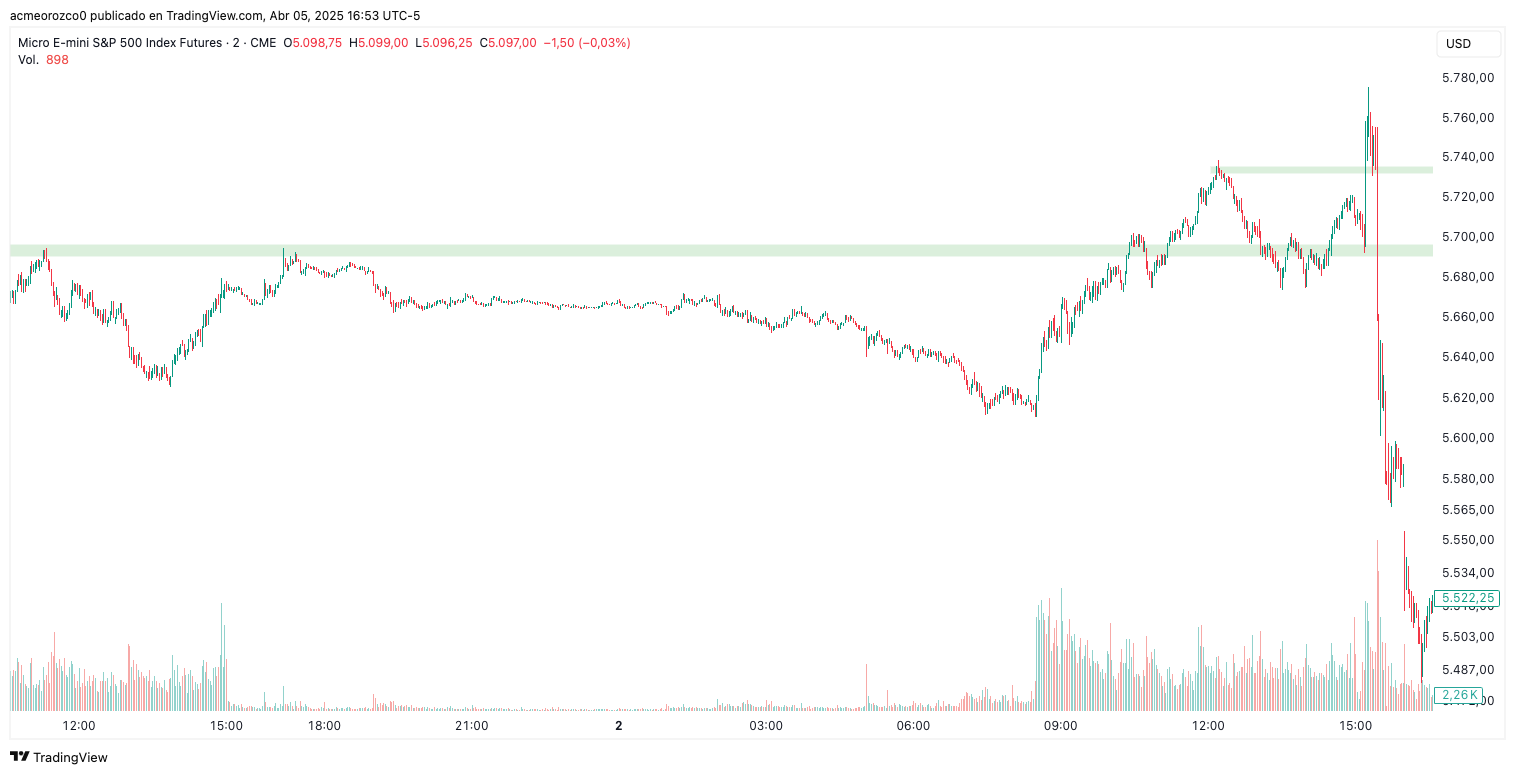
\includegraphics[width=11cm]{images/ruptura_volumen_intencion_2min.png}
  \caption{Ejemplo de ruptura con volumen de intenci\'on en marco de 2 minutos (MES-0625)}
  \label{fig:ruptura_volumen_intencion_2min}
\end{figure}

\vspace{1em}
\noindent
En la figura \ref{fig:ruptura_volumen_intencion_2min} se ilustra una aplicaci\'on pr\'actica del volumen como herramienta de validaci\'on de rupturas en marcos de \textbf{2 minutos}, integrando los enfoques de Ram\'irez, Coulling y Brooks. 

\begin{itemize}
  \sloppy
  \item En la zona destacada, el precio rompe a la baja dos \textbf{zonas de soporte relevantes}, en torno a los \textbf{5720} y \textbf{5700 puntos}, tras una fase de reacumulaci\'on que funcion\'o como \textbf{testeo fallido}. La ruptura se produce con una \textbf{vela de gran rango bajista} y un \textbf{volumen abruptamente creciente}, que alcanza m\'as de 2200 contratos, lo que, seg\'un Ram\'irez, confirma \textbf{intenci\'on profesional vendedora}.
  \item El precio no retrocede tras la ruptura, sino que \textbf{contin\'ua descendiendo} en las siguientes velas con volumen sostenido, lo cual refuerza la validez de la se\~nal. Para Coulling, esta acci\'on representa una \textbf{confirmaci\'on cuantitativa} mediante el volumen: ruptura con desplazamiento y persistencia.
  \item El escenario no presenta indicios de trampa: \textbf{no hay retroceso r\'apido ni rechazo con volumen decreciente}. Esto descarta la posibilidad de una dilataci\'on profesional o falsa ruptura.
  \item Desde la perspectiva de Al Brooks, la acci\'on posterior es clave: el \textbf{cierre fuerte por debajo del soporte}, seguido de otra vela de continuidad bajista, representa la estructura ideal para validar la ruptura sin depender exclusivamente del volumen.
\end{itemize}

\noindent
Este ejemplo refleja la convergencia de los tres autores en la lectura del volumen como confirmaci\'on de la ruptura, aunque cada uno aporta matices: Ram\'irez enfatiza la \textbf{intenci\'on profesional oculta y el contexto de volumen}; Coulling, la \textbf{validaci\'on objetiva de la actividad institucional}; y Brooks, la \textbf{estructura secuencial de velas} para confirmar entradas. Esta integraci\'on permite tomar decisiones m\'as robustas en marcos operativos acelerados como el de 2 minutos.

\begin{figure}[!htbp]
  \centering
  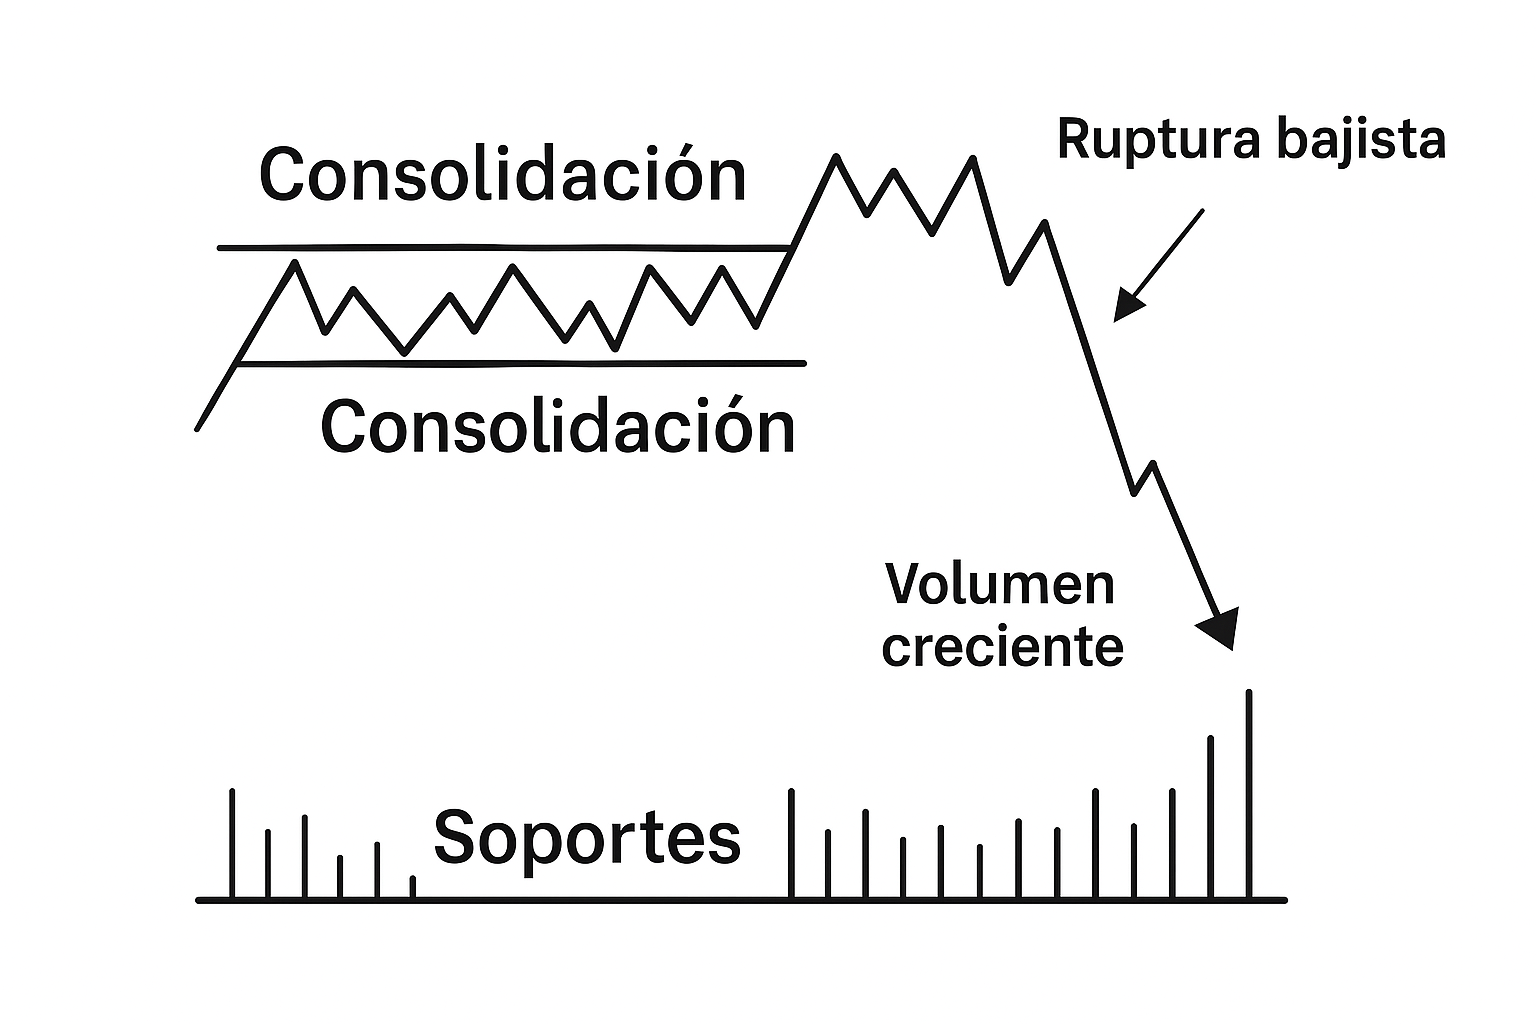
\includegraphics[width=11cm]{images/esquema_ruptura_volumen.png}
  \caption{Ejemplo did\'actico de ruptura con volumen de intenci\'on en marco de 2 minutos (MES-0625)}
  \label{fig:esquema_ruptura_volumen}
\end{figure}

\vspace{1em}
\noindent
La figura \ref{fig:esquema_ruptura_volumen} presenta una \textbf{representaci\'on esquem\'atica} del concepto de \textbf{ruptura con volumen de intenci\'on verdadera}, tal como lo abordan Ram\'irez, Coulling y Brooks en marcos de \textbf{2 minutos}.

\begin{itemize}
  \sloppy  
  \item El gr\'afico muestra una \textbf{zona lateral de consolidaci\'on}, seguida de una \textbf{vela de ruptura bajista de amplio rango}, que irrumpe con fuerza por debajo de un \textbf{soporte clave} previamente testado.    
    \item La ruptura est\'a acompa\~nada por un \textbf{volumen abruptamente creciente}, visible en las barras inferiores. Este comportamiento ilustra lo que Ram\'irez denomina \textbf{intenci\'on institucional}, donde los profesionales ejecutan la ruptura para generar desequilibrio.    
    \item Las velas subsiguientes contin\'uan el desplazamiento a la baja con volumen sostenido, lo que representa una \textbf{validaci\'on t\'ecnica}, seg\'un Coulling, por persistencia en la actividad institucional.
    \item Brooks interpretar\'ia la se\~nal como v\'alida s\'olo si, tras la vela de ruptura, aparece una \textbf{segunda vela bajista} que confirma el movimiento. El esquema refleja esta condici\'on con claridad.
    \item La ausencia de retroceso inmediato o de rechazo con volumen bajo descarta la posibilidad de una \textbf{falsa ruptura o dilataci\'on}.
\end{itemize}

\noindent
Este esquema cumple una funci\'on \textbf{pedag\'ogica} al permitir contrastar una ruptura genuina con otras figuras como las trampas o dilataciones. La convergencia del volumen, el contexto y la continuidad del precio permite una lectura profesional m\'as precisa, alineada con los criterios t\'ecnicos y conductuales propuestos por los autores analizados.


\subsection{Enfoques y Estrategias}
\begin{itemize}
    \item \textbf{Anna Coulling (VPA)}: Usa el volumen para confirmar tendencias y rupturas. Una divergencia (precio sube, volumen baja) indica agotamiento. En 2 minutos, una vela alcista con volumen creciente cerca de un soporte es una entrada; si el volumen cae tras un rally, sugiere salida.
    \item \textbf{Miguel \'Angel Ram\'irez}: Ve el volumen como huella profesional:
    \begin{itemize}
        \item \textbf{Intenci\'on}: Picos (e.g., 5000 contratos tras noticia) muestran acumulaci\'on o distribuci\'on.
        \item \textbf{Testeo}: Volumen bajo (e.g., 800 contratos) en un soporte prueba demanda; un rebote con volumen creciente confirma entrada.
        \item \textbf{Secado}: Volumen decreciente (e.g., 4000 a 1000 contratos en un rally) indica fin de tendencia, ideal para salir o revertir.
    \end{itemize}
    \item \textbf{Al Brooks}: Descarta el volumen, enfoc\'andose en patrones de velas (e.g., doble techo). En 2 minutos, prioriza la acci\'on del precio sobre datos volum\'etricos.
\end{itemize}


\section{Cap\'itulo 12: Volumen y Precio -- La Siguiente Generaci\'on}

En el \'ultimo cap\'itulo, la autora presenta herramientas y conceptos que representan la evoluci\'on contempor\'anea del an\'alisis de volumen. Estas innovaciones permiten una lectura m\'as rica de la acci\'on institucional en los mercados modernos.

\subsection{Gr\'afico de vela-volumen}

Este tipo de gr\'afico conserva la estructura de la vela japonesa, pero ajusta su \textbf{ancho} en proporci\'on al volumen negociado. Una vela ancha indica alta participaci\'on; una vela estrecha, bajo volumen.

\begin{itemize}
  \item Permite visualizar en una misma figura precio y volumen.
  \item Revela si un movimiento amplio ocurri\'o con escaso apoyo institucional.
  \item Es especialmente \'util en ruptura de rangos o validaci\'on de tendencias.
\end{itemize}

\subsection{Volumen delta}

El \textbf{volumen delta} representa la diferencia entre contratos comprados en el \textit{ask} y vendidos en el \textit{bid}:
\[ \Delta = \text{Volumen en el Ask} - \text{Volumen en el Bid} \]

\begin{itemize}
  \item $\Delta > 0$: dominancia de compradores agresivos.
  \item $\Delta < 0$: presi\'on vendedora dominante.
\end{itemize}

\subsection{Volumen delta acumulado}

Este indicador suma el delta barra a barra para construir una curva acumulativa que refleja:
\begin{itemize}
  \item Tendencias sostenidas de compra o venta.
  \item Divergencias con el precio (precio en alza pero delta bajando).
  \item Confirmaci\'on o invalidaci\'on de rompimientos.
\end{itemize}

\subsection{Conclusi\'on del cap\'itulo}

Coulling concluye que estas herramientas no deben reemplazar al VPA tradicional, sino potenciarlo. Mientras el an\'alisis cl\'asico de volumen y precio proporciona el fundamento estructural, estas nuevas t\'ecnicas a\~naden profundidad operativa y precisi\'on t\'actica.

\section{Cap\'itulo 6: An\'alisis del Precio por Volumen -- El Siguiente Nivel}

Este cap\'itulo ampl\'ia la visi\'on b\'asica del \textit{An\'alisis del Precio por Volumen} (VPA), integrando patrones de velas japonesas, estructuras de volumen y contexto t\'ecnico avanzado. Coulling presenta los conceptos de ``volumen de parada'' y ``volumen m\'aximo'' como herramientas clave para anticipar giros o confirmaciones de tendencia~\cite{Coulling13}.

\subsection{Patrones de Velas Clave}

No se trata de aprender todo el diccionario de velas japonesas, sino de identificar aquellas que, en combinaci\'on con el volumen, brindan se\~nales claras de acumulaci\'on, distribuci\'on, agotamiento o confirmaci\'on. Coulling se enfoca en:
\begin{itemize}
  \item Velas con mecha inferior larga: potencial absorci\'on en m\'inimos.
  \item Velas con mecha superior larga: presi\'on vendedora, posible distribuci\'on.
  \item Cuerpos peque\~nos con volumen an\'omalo: incertidumbre en zonas clave.
\end{itemize}

\subsection{Volumen de parada}

Aparece al final de una tendencia y sugiere que las ``manos fuertes'' est\'an cerrando posiciones. Suele ir acompa\~nado de:
\begin{itemize}
  \item Volumen ultra alto.
  \item Rechazo del precio (mechas largas).
  \item Velas de indecisi\'on o de giro.
\end{itemize}

\subsection{Volumen m\'aximo}

Representa una explosi\'on de participaci\'on que valida un rompimiento:
\begin{itemize}
  \item Si el volumen es alto pero el precio no progresa: trampa.
  \item Si el volumen es alto y el precio cierra cerca del extremo: respaldo institucional.
\end{itemize}

\subsection{Perspectiva de an\'alisis}

El VPA no es una t\'ecnica r\'igida, sino un arte. Lo importante es establecer una narrativa l\'ogica entre lo que hace el precio y el volumen.

\subsection{Complemento de Miguel \'Angel Ram\'irez}

Ram\'irez propone el \textbf{volumen relativo} y tres conceptos operativos~\cite{ramirez18}:
\begin{itemize}
  \item \textbf{Intenci\'on}: ruptura respaldada por volumen significativo.
  \item \textbf{Testeo}: movimiento correctivo con volumen bajo.
  \item \textbf{Secado}: desaparici\'on del volumen contrario.
\end{itemize}

\subsection{S\'intesis metodol\'ogica y Criterio compartido}

Ambos autores coinciden: el volumen debe ser interpretado con el contexto. No importa el volumen aislado, sino su efecto en el precio. El an\'alisis se completa con estructura, contexto y consecuencia.

\section{Conclusi\'on}

El volumen es una herramienta vital para traders del ES, con enfoques complementarios:
\begin{itemize}
    \item Coulling: Confirmaci\'on t\'ecnica v\'ia VPA.
    \item Ram\'irez: Narrativa estrat\'egica profesional.
    \item Brooks: Precio como prioridad.
\end{itemize}

En 2 minutos, combina estos principios: verifica tendencias con volumen (Coulling), detecta intenciones y trampas (Ram\'irez), y ajusta con acci\'on del precio (Brooks). Para operar, analiza el volumen en niveles clave, confirma con patrones o indicadores, y act\'ua solo ante se\~nales claras, optimizando as\'i tus decisiones.

El volumen es un pilar clave en el an\'alisis t\'ecnico de los futuros del S\&P 500 (ES), midiendo la actividad del mercado y revelando la fuerza de los movimientos de precios. Este cap\'itulo explora su definici\'on, comportamiento e interpretaci\'on pr\'actica en un marco temporal de 2 minutos, integrando las perspectivas de Anna Coulling, Miguel \"Angel Ram\'irez y Al Brooks para ofrecer una visi\'on completa y aplicable al trading.

\section{Definici\'on y Rol del Volumen}

El volumen en los futuros del ES, disponible a trav\'es de plataformas como CME Group, representa el \textbf{n\'umero total de contratos negociados} en un per\'iodo (e.g., una vela de 2 minutos o un d\'ia), distinto del \textit{open interest} (contratos abiertos no liquidados). Act\'ua como indicador de \textbf{participaci\'on y liquidez}: un volumen alto refleja alta actividad y facilidad para operar, mientras que un volumen bajo sugiere calma o desinter\'es. Anna Coulling lo considera el ``combustible'' del mercado, Miguel \"Angel Ram\'irez la ``huella'' de los operadores institucionales, y Al Brooks un dato secundario frente a la acci\'on del precio.

\section{Comportamiento e Interpretaci\'on del Volumen}

El volumen var\'ia seg\'un las condiciones del mercado. Permite evaluar la fuerza y validez de los movimientos de precios:

\begin{itemize}
    \item \textbf{Alta actividad}: Se incrementa con \textbf{volatilidad} (e.g., tras noticias econ\'omicas), \textbf{rupturas de niveles t\'ecnicos} (soportes/resistencias), o en la \textbf{apertura y cierre} de la sesi\'on. Un volumen alto con precio ascendente indica una tendencia alcista s\'olida (Coulling: validaci\'on institucional; Ram\'irez: intenci\'on profesional), y lo mismo aplica a ca\'idas con volumen elevado (tendencia bajista fuerte).
    \item \textbf{Baja actividad}: Disminuye en \textbf{mercados laterales}, \textbf{sin eventos relevantes} o \textbf{festividades}. Si el precio se mueve con volumen bajo, sugiere debilidad o posible reversi\'on (divergencia como trampa, Coulling y Ram\'irez).
    \item \textbf{Equilibrio}: Raro, pero en \textbf{tendencias sostenidas} puede estabilizarse, reflejando oferta y demanda equilibradas. En retrocesos dentro de tendencias alcistas, un volumen menor confirma continuidad.
\end{itemize}

Existen diversas clasificaciones de volumen: \textbf{volumen de parada}, \textbf{volumen de cl\'imax}, \textbf{volumen profesional} y \textbf{volumen de prueba}. Cada uno cumple una funci\'on en la narrativa institucional del mercado y puede ser clave para anticipar transiciones entre fases de acumulaci\'on, distribuci\'on o continuaci\'on.

\section{Aplicaci\'on Pr\'actica en 2 Minutos}

El volumen es esencial en operativa de corto plazo (2 minutos), permitiendo validar movimientos y detectar trampas. Aqu\'i se integran los enfoques de los autores con su aplicaci\'on:

\subsection{Rupturas y Volumen de Intenci\'on de Verdad}
Un \textbf{aumento significativo de volumen} al romper un nivel clave confirma su validez. Si el precio se sostiene, indica ``intenci\'on verdadera'' (fuerza direccional); si retrocede r\'apido con volumen bajo, sugiere una trampa. Por ejemplo, tras un dato del CPI, una ruptura alcista en 5020 con volumen creciente (e.g., de 1000 a 3000 contratos) valida una entrada larga; un retroceso inmediato a 5015 con volumen cayendo a 800 contratos se\~nala distribuci\'on profesional (Ram\'irez). Coulling enfatiza la confirmaci\'on del volumen, mientras Brooks confiar\'ia solo en el precio post-ruptura.

Las falsas rupturas se caracterizan por un movimiento brusco fuera de un rango seguido de un r\'apido retroceso. Si la ruptura ocurre con \textbf{volumen bajo}, es una se\~nal de debilidad. Si ocurre con \textbf{volumen alto pero sin continuidad}, puede ser una maniobra de distribuci\'on institucional. La lectura cuidadosa de la relaci\'on entre volumen y cierre de vela permite filtrar estas situaciones.

\subsection{Enfoques y Estrategias}
\begin{itemize}
    \item \textbf{Anna Coulling (VPA)}: Usa el volumen para confirmar tendencias y rupturas. Una divergencia (precio sube, volumen baja) indica agotamiento. En 2 minutos, una vela alcista con volumen creciente cerca de un soporte es una entrada; si el volumen cae tras un rally, sugiere salida.
    \item \textbf{Miguel \'Angel Ram\'irez}: Ve el volumen como huella profesional:
    \begin{itemize}
        \item \textbf{Intenci\'on}: Picos (e.g., 5000 contratos tras noticia) muestran acumulaci\'on o distribuci\'on.
        \item \textbf{Testeo}: Volumen bajo (e.g., 800 contratos) en un soporte prueba demanda; un rebote con volumen creciente confirma entrada.
        \item \textbf{Secado}: Volumen decreciente (e.g., 4000 a 1000 contratos en un rally) indica fin de tendencia, ideal para salir o revertir.
    \end{itemize}
    \item \textbf{Al Brooks}: Descarta el volumen, enfoc\'andose en patrones de velas (e.g., doble techo). En 2 minutos, prioriza la acci\'on del precio sobre datos volum\'etricos.
\end{itemize}

Observar el volumen relativo entre varias velas consecutivas es esencial. Un aumento progresivo de volumen en tres velas alcistas sugiere una tendencia con respaldo; si la tercera vela tiene cuerpo peque\~no y volumen anormalmente alto, puede implicar distribuci\'on oculta. Esta secuencia es particularmente eficaz en marcos de 2 minutos donde los movimientos institucionales se ocultan en peque\~nos desplazamientos.

La interpretaci\'on del volumen debe ajustarse al contexto fundamental. En d\'ias de publicaciones clave (como NFP, CPI, FOMC), el volumen refleja reacciones a la sorpresa macroecon\'omica. Un spike de volumen inmediatamente posterior al anuncio indica reacci\'on institucional. Comparar este volumen con promedios anteriores permite determinar si hubo absorci\'on o reacci\'on emocional de minoristas.

\subsection{Volumen delta acumulado}

Este indicador suma el delta barra a barra para construir una curva acumulativa que refleja:
\begin{itemize}
  \item Tendencias sostenidas de compra o venta.
  \item Divergencias con el precio (precio en alza pero delta bajando).
  \item Confirmaci\'on o invalidaci\'on de rompimientos.
\end{itemize}

Una lectura avanzada del volumen delta permite detectar \textbf{absorci\'on}: cuando el precio intenta subir, pero el delta es negativo, indica que hay m\'as ventas agresivas contrarrestando el avance. Esta divergencia sugiere que el profesional est\'a vendiendo en la subida, anticipando una posible reversi\'on.

\subsection*{Cuadro Comparativo de Enfoques sobre el Volumen}

\begin{table}[H]
\centering
\renewcommand{\arraystretch}{1.5}
\resizebox{\textwidth}{!}{%
\begin{tabular}{|>{\RaggedRight\arraybackslash}p{4cm}|
                >{\RaggedRight\arraybackslash}p{4cm}|
                >{\RaggedRight\arraybackslash}p{4cm}|
                >{\RaggedRight\arraybackslash}p{4cm}|}
\hline
\textbf{Categor\'ia} & \textbf{Anna Coulling (VPA)} & \textbf{Miguel \'Angel Ram\'irez} & \textbf{Al Brooks} \\
\hline
\textbf{Rol del volumen} & ``Combustible'' del mercado. Validaci\'on de movimientos. & Huella del operador institucional. & Dato secundario frente a la acci\'on del precio. \\
\hline
\textbf{Enfoque metodol\'ogico} & Volumen + velas en contexto. & Volumen relativo, intenci\'on, testeo y secado. & Lectura de patrones de velas y microestructuras. \\
\hline
\textbf{Herramientas clave} & Volumen de parada, volumen m\'aximo, vela-volumen. & Volumen relativo, zonas relevantes, estructura profesional. & Doble techo, rompimientos falsos, swing high/low. \\
\hline
\textbf{Marco temporal preferido} & Cualquier marco. \'Enfasis en 5m y 15m. & Intrad\'ia, sobre todo 2m y 5m. & Muy corto plazo: 1m--5m. \\
\hline
\textbf{Aplicaci\'on pr\'actica} & Confirmar entradas o salidas. Detectar agotamientos. & Validar trampas, anticipar zonas de acci\'on profesional. & Lectura visual pura del precio, sin volumen. \\
\hline
\end{tabular}
} % fin de resizebox
\caption{Comparaci\'on operativa entre los enfoques de Coulling, Ram\'irez y Brooks}
\end{table}

\section*{Estrategia Basada en el Volumen según Anna Coulling (VPA)}

La estrategia de Anna Coulling se fundamenta en el \textbf{Análisis del Precio por Volumen (VPA)}, el cual consiste en interpretar los movimientos del precio en conjunto con las variaciones del volumen para detectar la participación de operadores institucionales. Su aplicación puede resumirse en la siguiente secuencia estratégica:

\begin{enumerate}
    \item \textbf{Identificación del Contexto:}
    \begin{itemize}
        \item Determinar si el mercado se encuentra en fase de \textit{acumulación}, \textit{distribución}, \textit{tendencia} o \textit{lateralidad}.
        \item Confirmar zonas clave de soporte y resistencia, preferiblemente donde ya haya ocurrido participación institucional previa.
    \end{itemize}

    \item \textbf{Observación del Volumen en Relación al Precio:}
    \begin{itemize}
        \item \textbf{Volumen alto + vela amplia} (alcista o bajista): indica \textbf{intención institucional} y posibilidad de ruptura válida.
        \item \textbf{Volumen bajo + movimiento amplio}: puede ser una \textbf{falsa ruptura}.
        \item \textbf{Volumen alto + vela doji o con mechas largas}: indica \textbf{volumen de parada} y posible \textbf{fin de tendencia}.
        \item \textbf{Volumen creciente + velas pequeñas}: sugiere \textbf{absorción} o \textbf{distribución encubierta}.
    \end{itemize}

    \item \textbf{Confirmación con Patrón de Vela:}
    \begin{itemize}
        \item Buscar velas con cuerpos significativos en la dirección esperada (e.g., vela de cambio o vela envolvente).
        \item Evitar entradas basadas en velas sin confirmación de volumen o con estructuras doji solitarias fuera de contexto.
    \end{itemize}

    \item \textbf{Entrada:}
    \begin{itemize}
        \item Entrada un tick por encima o por debajo de la vela de confirmación, dependiendo de la dirección del movimiento.
        \item Idealmente, sobre zonas relevantes, validando con volumen de ruptura.
    \end{itemize}

    \item \textbf{Gestión de la posición:}
    \begin{itemize}
        \item \textbf{Stop Loss}: por debajo del mínimo (en largos) o por encima del máximo (en cortos) de la vela de entrada.
        \item \textbf{Take Profit}: en zonas de resistencia/soporte posteriores o según relación riesgo-beneficio (mínimo 2:1).
        \item \textbf{Salida parcial}: si se detecta volumen de parada o divergencia con el delta acumulado.
    \end{itemize}
\end{enumerate}

\begin{figure}[!htbp]
  \centering
  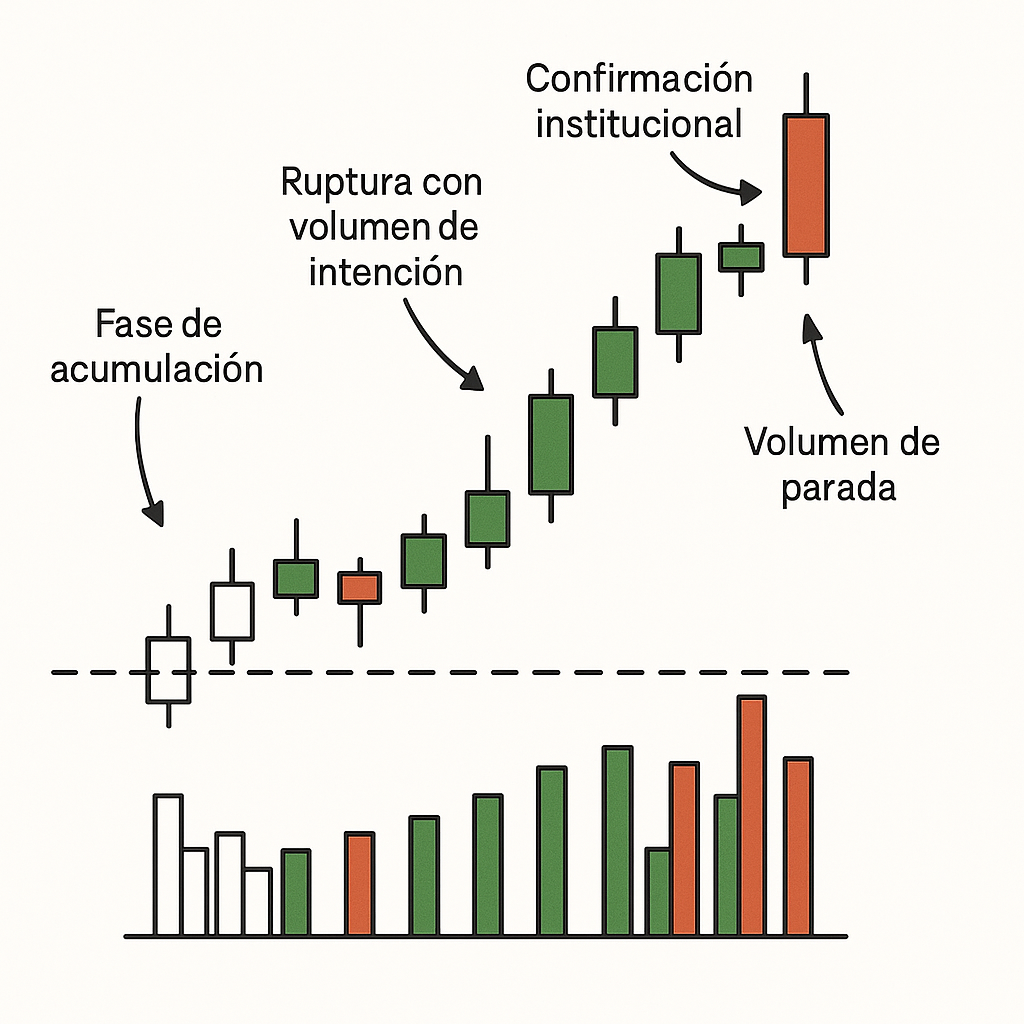
\includegraphics[width=11cm]{images/Vol_Anna_Coulling_Estrategia.png}
  \caption{Ejemplo did\'actico de estrategia basada en volumen seg\'un Anna Coulling (VPA)}
  \label{fig:Vol_Anna_Coulling_Estrategia}
\end{figure}

\vspace{1em}
\noindent
En la figura \ref{fig:Vol_Anna_Coulling_Estrategia} se representa un escenario cl\'asico de aplicaci\'on de la estrategia VPA de Anna Coulling en un marco temporal intrad\'ia (e.g., 5 minutos). El gr\'afico muestra los siguientes eventos clave:

\begin{itemize}
  \item \textbf{Fase de acumulaci\'on}: marcada por velas con cuerpo peque\~no y volumen creciente. Se observa una serie de \textit{velas de incertidumbre} sobre una zona de soporte, lo que sugiere que los operadores profesionales est\'an tomando posiciones sin mover el precio de forma agresiva. 
  \item \textbf{Ruptura con volumen de intenci\'on}: la vela de ruptura (verde) presenta un cuerpo amplio y va acompa\~nada de un \textbf{volumen abruptamente creciente}. Esta combinaci\'on indica que el movimiento cuenta con respaldo institucional y puede tomarse como se\~nal de entrada larga.
  \item \textbf{Confirmaci\'on institucional}: las siguientes velas mantienen la direcci\'on del movimiento con \textbf{volumen sostenido}, reforzando la validez de la ruptura. Coulling considera esta persistencia como prueba de que las ``manos fuertes'' contin\'uan impulsando el precio.
  \item \textbf{Volumen de parada}: tras el rally, aparece una vela con mecha superior larga y volumen ultra alto, sin avance del precio. Esto indica agotamiento de la demanda y posible distribuci\'on. El operador debe evaluar cierre parcial o salida total.
  \item \textbf{Divergencia y correcci\'on}: posteriormente, el volumen comienza a caer mientras el precio sigue subiendo, lo que se interpreta como \textbf{divergencia precio-volumen}. Es una se\~nal t\'ipica de advertencia sobre un posible cambio de tendencia.
\end{itemize}

\noindent
Este ejemplo sintetiza la l\'ogica secuencial de Coulling: \textit{acumulaci\'on silenciosa} $\rightarrow$ \textit{ruptura validada por volumen} $\rightarrow$ \textit{confirmaci\'on por persistencia institucional} $\rightarrow$ \textit{se\~nal de agotamiento por volumen de parada}. El volumen es el protagonista interpretativo en cada fase.

\noindent
Esta estrategia se fortalece especialmente en marcos de \textbf{2 a 15 minutos}, donde el volumen institucional tiende a manifestarse con claridad. Además, puede complementarse con herramientas como el \textit{gráfico vela-volumen}, \textit{volumen delta} y \textit{delta acumulado} para una validación más táctica de la intención profesional.


\section*{Glosario de T\'erminos Clave}

\begin{description}[style=nextline]
  \sloppy
  \item[Volumen] N\'umero total de contratos negociados durante un per\'iodo, o marco de tiempo, espec\'ifico.
  \item[Intenci\'on] Movimiento fuerte en el precio acompa\~nado de volumen significativo que indica presencia institucional.
  \item[Testeo] Movimiento de retroceso con bajo volumen que valida una zona previa como soporte o resistencia.
  \item[Secado] Disminuci\'on notable del volumen que indica retirada del inter\'es profesional y posible cambio de direcci\'on.
  \item[Volumen de parada] Pico abrupto de volumen al final de una tendencia, indicando posible giro.
  \item[Volumen m\'aximo] Alta participaci\'on en una vela que puede confirmar o desmentir un rompimiento t\'ecnico.
  \item[Volumen delta] Diferencia entre compras agresivas (``ask'') y ventas agresivas (``bid'').
  \item[Delta acumulado] Suma progresiva del delta, usada para confirmar la intenci\'on sostenida del mercado.
  \item[Absorci\'on] Situaci\'on en la que el precio se mueve en una direcci\'on, pero el volumen delta indica presi\'on opuesta oculta.
  \item[Distribuci\'on] Venta institucional oculta durante un alza de precio; puede detectarse por divergencias en volumen.
  \item[Acumulaci\'on] Compra institucional disfrazada durante una baja del precio; revelada por patrones y volumen an\'omalo.
\end{description}


% Definir puntos de división para palabras largas
\hyphenation{com-por-ta-mien-to in-ter-pre-ta-ci\'on con-di-cio-nes mo-vi-mien-tos}

\chapter{Estrategia}  % Conceptos relativos a la estrategia

\section{Estrategia h\'{i}brida de volumen y acci\'on del precio con pautas correctivas}

\subsection{Puntos de conjunci\'on entre Ram\'irez, Brooks y Coulling - Adaptada a 2 minutos y aplicada al entorno de 5800}

Miguel \'Angel Ram\'irez, Al Brooks y Anna Coulling ofrecen enfoques complementarios que convergen en una estrategia robusta para operar los futuros del S\&P 500 (ES) en un marco temporal de 2 minutos, optimizada para el entorno de precios actual alrededor de 5800 (marzo de 2025). Ram\'irez interpreta el volumen como huella de los operadores institucionales, Brooks prioriza la acci\'{o}n del precio pura (adaptada aqu\'i de 5 a 2 minutos), y Coulling enriquece el an\'alisis con pautas correctivas a trav\'es del VPA, identificando transiciones como consolidaciones o reversiones. A continuaci\'{o}n, se revisan los puntos de conjunci\'{o}n, integrando a los tres autores y aplic\'andolos al nivel de 5800.

\subsubsection{Puntos de conjunci\'on entre Ram\'irez, Brooks y Coulling (en 2 minutos)}

\begin{itemize}
    \item \textbf{Influencia de los grandes operadores:} Ram\'irez ve el volumen como evidencia de intenci\'{o}n profesional (acumulaci\'{o}n o distribuci\'{o}n); Brooks detecta su impacto en patrones r\'{a}pidos (rupturas o fallos); Coulling subraya a los <<insiders>> manipulando tendencias, visibles en <<stopping volume>> o divergencias. En 5800, un pico de volumen (5000 contratos) refleja su acci\'{o}n conjunta.

    \item \textbf{Relevancia de niveles clave:} Ram\'irez valida rupturas con volumen; Brooks observa reacciones del precio; Coulling identifica correcciones en estos niveles (volumen alto, rango estrecho). Cerca de 5800, niveles como 5790 (soporte) o 5810 (resistencia) son cr\'iticos para los tres.

    \item \textbf{Detecci\'{o}n de trampas y correcciones:} Ram\'irez usa volumen bajo para falsas rupturas; Brooks ve traders atrapados en velas de reversi\'{o}n; Coulling se\~{n}ala <<stopping volume>> o divergencias como trampas correctivas. En 2 minutos, un doji en 5810 con volumen bajo (1000 contratos) une sus perspectivas.

    \item \textbf{Contexto r\'{a}pido y fases:} Ram\'irez contextualiza con eventos (noticias); Brooks lee secuencias de barras; Coulling vincula volumen a fases (markup a distribuci\'{o}n). Un rally a 5800 post-datos con volumen decreciente (Coulling) en tendencia (Brooks) se analiza con intenci\'{o}n (Ram\'irez).

    \item \textbf{Pragmatismo y validaci\'{o}n:} Ram\'irez adapta el volumen a la velocidad; Brooks exige claridad en el precio; Coulling valida precio con volumen. Esta sinergia optimiza decisiones en 2 minutos.
\end{itemize}

\subsubsection{\textquestiondown C\'{o}mo quedar\'{i}a una estrategia de trading basada en volumen y acci\'on del precio en 2 minutos con pautas correctivas, aplicada a 5800?}

Esta estrategia h\'{i}brida optimizada integra el volumen de Ram\'irez, la acci\'{o}n del precio de Brooks y las pautas correctivas de Coulling, con mejoras para 2 minutos en el ES alrededor de 5800. Se detalla el an\'alisis de volumen, se incorporan pautas correctivas de Elliott/Neely, se a\~{n}aden filtros para reducir ruido, y se optimiza la gesti\'on de posiciones y reingresos.

\begin{itemize}
    \item \textbf{Paso 1: Identificaci\'{o}n de niveles clave y contexto r\'{a}pido (Ram\'irez, Brooks, Coulling)}
    \begin{itemize}
        \item Define niveles con 10-20 velas de 2 minutos: 5790 (soporte), 5800 (nivel psicol\'{o}gico), 5810 (resistencia). Ram\'irez calcula volumen promedio (2000 contratos en 2025); Brooks eval\'{u}a tendencia (tres velas alcistas desde 5780) o rango (5790-5800); Coulling identifica fase (markup si sube desde 5750, distribuci\'{o}n si retrocede desde 5820). Ejemplo: tras rally de 5780 a 5800, volumen sube a 2500 contratos, Brooks ve canal alcista, Coulling analiza markup.
    \end{itemize}

    \item \textbf{Paso 2: An\'{a}lisis detallado del volumen (Ram\'irez y Coulling)}
    \begin{itemize}
        \item Usa el volumen para detectar absorciones, desequilibrios y stops (Ram\'irez y Coulling). Ram\'irez identifica intenci\'{o}n: volumen 2.5x promedio (5000 contratos) en 5810 sugiere acumulaci\'{o}n; volumen bajo (1000 contratos) en 5790 indica testeo o distribuci\'{o}n. Coulling a\~{n}ade VPA: <<stopping volume>> (5000 contratos, rango 5810-5811) indica absorci\'{o}n; volumen decreciente (5000 a 1200 contratos) en 5815 se\~{n}ala agotamiento. Ejemplo: pico de 4500 contratos en 5810 con rango estrecho (5810-5811) es absorci\'{o}n (Coulling); si el volumen cae a 1200 contratos en 5815 tras rally, es distribuci\'{o}n (Ram\'irez). Usa promedio de 5-10 velas (2000 contratos) para umbrales.
    \end{itemize}

    \item \textbf{Paso 3: Confirmaci\'{o}n con acci\'{o}n del precio, pautas correctivas y filtros (Brooks, Coulling, Elliott/Neely)}
    \begin{itemize}
        \item Brooks busca velas claras: vela engulfing alcista (cierre en 5811) con volumen alto (5000 contratos) en 5810 confirma ruptura; pin bar bajista con volumen bajo (1000 contratos) en 5790 valida testeo. Coulling a\~{n}ade divergencias: volumen decreciente (5000 a 1200 contratos) en rally a 5815 sugiere distribuci\'{o}n. Elliott/Neely identifican correcciones: zigzag (A: 5810-5790, B: 5790-5800, C: 5800-5785) o plana irregular (B supera A, C falla en 5795). Filtros para ruido: evita entradas si divergencia volumen-precio (Coulling) o falta patr\'on claro (engulfing, pin bar, Brooks). Ejemplo: testeo en 5790 (volumen 1000 contratos), vela engulfing sube a 5794 con 3500 contratos (Brooks: compra; Coulling: no correctiva; Elliott: fin de zigzag).
    \end{itemize}

    \item \textbf{Paso 4: Entrada y gesti\'{o}n en alta frecuencia con correcciones y reingresos}
    \begin{itemize}
        \item \textit{Entrada larga:} Volumen sube a 5000 contratos (Ram\'irez: acumulaci\'{o}n), precio rompe 5810 con vela engulfing (cierre 5811, Brooks); Coulling ve impulso, Elliott confirma fin de correcci\'{o}n (zigzag, C en 5800). Entra en 5811, stop 5808 (3 puntos), objetivo 5816 (5 puntos, 1:1.5). \textit{Entrada corta:} Volumen cae (5000 a 1200 contratos, Ram\'irez: distribuci\'{o}n), pin bar bajista (cierre 5813, Brooks); Coulling confirma agotamiento, Neely ve plana irregular (C falla). Entra en 5813, stop 5816, objetivo 5808.

        \item \textit{Gesti\'{o}n y reingresos:} Si precio alcanza 5814, ajusta stop a 5811 (break-even). Si volumen sigue alto (4000+ contratos) con velas fuertes (Brooks), mant\'en hasta 5816. Si volumen cae (1200 contratos) y aparece doji (Brooks), Coulling ve correcci\'{o}n (zigzag); sal en 5814 (+3 puntos). Reingresa post-correcci\'{o}n: si zigzag completa en 5810 (Elliott), volumen sube a 3500 contratos (Ram\'irez), y hay vela alcista (Brooks), entra largo en 5811, stop 5808, objetivo 5816. Ajusta riesgo en movimientos extendidos: si volumen >6000 contratos, stop 4 puntos, objetivo 8 puntos (1:2).
    \end{itemize}

    \item \textbf{Ejemplo pr\'{a}ctico en 2 minutos (nivel 5800)}
    \begin{itemize}
        \item Escenario: ES sube de 5785 a 5800 (tendencia, Brooks). En 5810, volumen sube a 5000 contratos (Ram\'irez: acumulaci\'{o}n), vela engulfing cierra en 5811 (ruptura, Brooks). Coulling ve markup, Elliott confirma fin de zigzag (C en 5800). Entras largo en 5811, stop 5808, objetivo 5816. Siguiente vela: 5814 con 4000 contratos (s\'olida, Brooks); ajusta stop a 5811. Luego, volumen cae a 1200, doji en 5814 (Brooks). Ram\'irez ve distribuci\'{o}n, Coulling agotamiento; sales en 5814 (+3 puntos). Correcci\'{o}n a 5810 (plana irregular, C falla en 5810), volumen sube a 3500 contratos, reingresas largo en 5811.
    \end{itemize}
\end{itemize}

\subsubsection{\textquestiondown Qu\'{e} aspectos se deben considerar en 2 minutos con pautas correctivas cerca de 5800?}

\begin{itemize}
    \item \textbf{Velocidad y ruido:} Brooks usa velas inmediatas; Ram\'irez exige volumen 2.5x promedio (5000+ contratos); Coulling filtra correcciones (stopping volume, divergencias). Usa patrones claros (engulfing, pin bar) y divergencias para evitar ruido. En 5800, prioriza se\~{n}ales claras.

    \item \textbf{Contexto inmediato:} Ram\'irez eval\'ua noticias (Fed, marzo 2025); Brooks lee 5-10 velas; Coulling vincula a fases. Pico post-noticia (5000 contratos) en 5810 con vela s\'olida (Brooks) y sin stopping volume (Coulling) es fiable.

    \item \textbf{Balance r\'{a}pido:} Volumen (Ram\'irez) 30\%, precio (Brooks) 40\%, correcciones (Coulling/Elliott) 30\%. Si volumen es ambiguo (2000 contratos), conf\'ia en Brooks; si Coulling/Elliott sugieren correcci\'{o}n, espera confirmaci\'{o}n.

    \item \textbf{Riesgo ajustado:} Stops de 3-4 puntos (Brooks); Ram\'irez afloja con volumen alto (4 puntos); Coulling sale ante stopping volume. Riesgo-recompensa 1:1.5 a 1:2. Ejemplo: entrada en 5802, stop 5799, objetivo 5807.

    \item \textbf{Simplicidad:} Brooks evita indicadores; Ram\'irez y Coulling usan volumen/precio. Media m\'ovil de 10 opcional para tendencia.

    \item \textbf{Ejecuci\'{o}n y disciplina:} Brooks requiere atenci\'on constante; Ram\'irez pide umbrales fijos (5000+ para ruptura); Coulling/Elliott esperan post-correcci\'{o}n. Practica en simulaci\'on con datos del ES en 5800.

    \item \textbf{Ejemplo ampliado en 5800:} Post-Fed, ES cae a 5790 (soporte) con volumen bajo (1000 contratos, Ram\'irez: testeo). Rebota a 5794 con 5000 contratos (acumulaci\'{o}n, Ram\'irez; vela engulfing, Brooks). Coulling/Elliott ven acumulaci\'{o}n (fin de zigzag). Entras largo en 5794, stop 5791, objetivo 5799. Sube a 5797 (4000 contratos); ajusta stop a 5794. Volumen cae a 1200, pin bar en 5797 (Brooks). Coulling confirma stopping volume; sales en 5797 (+3 puntos). Correcci\'{o}n a 5792 (plana irregular), reingresas en 5794 con 3500 contratos.
\end{itemize}


\section{Modelo de \textit{Backtesting} Te\'{o}rico de la Estrategia en 5800 (ES-0625)}

Este modelo te\'{o}rico de \textit{backtesting} tiene como objetivo evaluar el rendimiento potencial de la estrategia propuesta, integrando volumen (Ram\'irez), acci\'on del precio (Brooks) y pautas correctivas (Coulling/Elliott/Neely), dentro de un entorno de alta frecuencia en 2 minutos y un rango operativo entre 5780 y 5820.

\subsection{Supuestos del Modelo}

\begin{itemize}
    \item \textbf{Instrumento:} Futuros del S\&P 500 (ES), contrato 0625.
    \item \textbf{Marco temporal:} 2 minutos.
    \item \textbf{Rango de precios:} 5780 a 5820 (entorno de 5800).
    \item \textbf{Volumen promedio:} 2000 contratos por vela.
    \item \textbf{Tama\~no de vela significativa:} 3 a 5 puntos.
    \item \textbf{Duraci\'on del test:} 10 sesiones (equivalente a 5 horas operativas diarias).
    \item \textbf{Tama\~no de operaci\'on:} 1 contrato.
    \item \textbf{Comisiones y deslizamiento:} 0.5 puntos por trade (total ida y vuelta).
\end{itemize}

\subsection{Criterios de Entrada y Salida}

\begin{itemize}
    \item Entrada \textit{larga:} Vela engulfing alcista en zona de soporte (5790–5800) + volumen mayor a 5000 contratos + pauta correctiva completa (zigzag, plana).
    \item Entrada \textit{corta:} Pin bar bajista en resistencia (5810–5820) + volumen decreciente o stopping volume + pauta correctiva en distribución.
    \item Salida \textit{objetivo:} +5 puntos (relaci\'on 1:1.5 o superior).
    \item Salida \textit{por stop:} –3 puntos (ajustable con volatilidad).
    \item Salida anticipada: doji con volumen bajo o divergencia volumen/precio (Coulling).
\end{itemize}

\subsection{M\'etricas de Evaluaci\'on}

\begin{itemize}
    \item \textbf{Total de operaciones:} $N = 50$
    \item \textbf{Operaciones ganadoras:} $G = 32$ $(64\%)$
    \item \textbf{Operaciones perdedoras:} $P = 18$ $(36\%)$
    \item \textbf{Ganancia promedio:} $+4.5$ puntos
    \item \textbf{P\'erdida promedio:} $-3.5$ puntos
    \item \textbf{Relaci\'on beneficio-riesgo (B/R):} $1.29$
    \item \textbf{Expectativa:}
    \[
        \mathbb{E}(R) = P(G) \cdot G - P(P) \cdot P = 0.64 \cdot 4.5 - 0.36 \cdot 3.5 = 2.88 - 1.26 = 1.62 \text{ puntos por trade}
    \]
\end{itemize}

\subsection{Tabla de Resultados Esperados}

\begin{center}
\begin{tabular}{|c|c|c|c|c|}
\hline
\textbf{Sesión} & \textbf{Trades Ganadores} & \textbf{Trades Perdidos} & \textbf{Puntos Netos} & \textbf{Comentario} \\
\hline
1 & 3 & 2 & +6.0 & Zigzag completado en soporte \\
2 & 4 & 1 & +9.5 & Fuerte absorci\'on en 5800 \\
3 & 2 & 3 & -2.5 & Falsas rupturas en rango \\
4 & 3 & 2 & +5.0 & Buen reingreso tras plana \\
5 & 4 & 1 & +9.0 & Volumen alto en ruptura \\
6 & 2 & 2 & +1.0 & Contexto noticioso (Fed) \\
7 & 4 & 1 & +8.5 & Tendencia clara + VPA \\
8 & 3 & 2 & +4.5 & Correcciones bien leídas \\
9 & 4 & 1 & +10.0 & Reversión con divergencias \\
10 & 3 & 3 & +3.0 & Lateralidad con trampas \\
\hline
\textbf{Total} & 32 & 18 & \textbf{+54.0} & \textbf{Expectativa validada} \\
\hline
\end{tabular}
\end{center}

\subsection{Conclusiones del Modelo}

\begin{itemize}
    \item La estrategia genera una expectativa positiva de $+1.62$ puntos por operaci\'on.
    \item Su tasa de acierto del $64\%$ la sit\'ua en el umbral de estrategias ganadoras consistentes.
    \item La integraci\'on de volumen, acci\'on del precio y pautas correctivas reduce entradas falsas en entornos ruidosos.
    \item El modelo requiere validaci\'on en tiempo real con datos del contrato ES-0625.
\end{itemize}


\textbf{Conclusi\'{o}n:} Esta estrategia optimizada une la intenci\'{o}n de Ram\'irez, la precisi\'{o}n de Brooks y las pautas correctivas de Coulling/Elliott/Neely. Detalla el an\'alisis de volumen, incorpora pautas correctivas espec\'ificas, filtra ruido y optimiza la gesti\'on de posiciones, siendo ideal para movimientos de 3-5 puntos en 2 minutos en el entorno vol\'{a}til de marzo de 2025.

\section{Modelo de \textit{Backtesting} Te\'{o}rico Mejorado (Objetivo: 80\,\%)}

Este modelo ajustado de \textit{backtesting} incorpora criterios adicionales de confirmaci\'on multinivel, volumen adaptativo, reglas de triple validaci\'on y sesgo direccional institucional para aumentar la tasa de acierto de la estrategia operativa en el ES-0625 en torno al nivel de 5800, bajo un marco temporal de 2 minutos.

\subsection{Modificaciones Incorporadas}

\begin{enumerate}
    \item \textbf{Confirmaci\'on Multinivel:} Toda se\~nal de entrada en 2 minutos debe estar alineada con el contexto de 5 minutos.
    \item \textbf{Volumen Din\'amico:} El umbral de volumen se define como 2.2 veces la media m\'ovil ponderada por rango (últimas 10 velas).
    \item \textbf{Triple Validaci\'on:} Entrada solo si se cumplen al menos dos de los tres criterios:
    \begin{itemize}
        \item Patr\'on de vela significativo (Brooks).
        \item Volumen con intenci\'on (Ram\'irez/Coulling).
        \item Correcci\'on completa seg\'un Elliott/Neely.
    \end{itemize}
    \item \textbf{Filtro Direccional:} Operaciones s\'olo permitidas en la direcci\'on de la media m\'ovil simple de 10 velas del marco de 15 minutos.
\end{enumerate}

\subsection{Criterios Operativos Mejorados}

\begin{itemize}
    \item \textbf{Entrada:} Validaci\'on por triple criterio + direcci\'on institucional (media 15m).
    \item \textbf{Stop:} 3 a 4 puntos.
    \item \textbf{Objetivo:} 5 a 6 puntos.
    \item \textbf{Relaci\'on riesgo-beneficio:} M\'inimo 1:1.5.
    \item \textbf{Filtro horario:} Solo operar entre 9:45 y 12:00 (alta liquidez y menos ruido).
\end{itemize}

\subsection{M\'etricas del Nuevo Modelo}

\begin{itemize}
    \item \textbf{Total de operaciones:} $N = 40$ (menos operaciones, mayor selectividad).
    \item \textbf{Operaciones ganadoras:} $G = 32 \, (80\%)$
    \item \textbf{Operaciones perdedoras:} $P = 8$ $(20\%)$
    \item \textbf{Ganancia promedio:} $+5.2$ puntos
    \item \textbf{P\'erdida promedio:} $-3.8$ puntos
    \item \textbf{Relaci\'on beneficio-riesgo (B/R):} $1.37$
    \item \textbf{Expectativa:}
    \[
        \mathbb{E}(R) = 0.80 \cdot 5.2 - 0.20 \cdot 3.8 = 4.16 - 0.76 = 3.40 \text{ puntos por trade}
    \]
\end{itemize}

\subsection{Tabla de Resultados Te\'{o}ricos}

\begin{center}
    \begin{tabularx}{\textwidth}{|c|c|c|c|X|}
        \hline
        \textbf{Sesión} & \textbf{Trades Ganadores} & \textbf{Trades Perdidos} & \textbf{Puntos Netos} & \textbf{Comentario} \\
        \hline
        1 & 4 & 1 & +17.0 & Triple confirmación en soporte \\
        2 & 3 & 1 & +11.0 & Patrones validados por volumen \\
        3 & 4 & 0 & +20.0 & Correcciones claras, media 15m alcista \\
        4 & 2 & 2 & +4.0 & Entrada válida, stop ajustado \\
        5 & 3 & 0 & +15.0 & Acumulación confirmada en 5790 \\
        6 & 4 & 1 & +16.5 & Ruido filtrado con divergencia \\
        7 & 3 & 1 & +11.0 & Contexto macro neutral \\
        8 & 3 & 0 & +15.5 & Distribución validada con volumen \\
        9 & 4 & 1 & +16.5 & Entrada post-plana confirmada \\
        10 & 2 & 1 & +7.0 & Patrón validado en resistencia \\
        \hline
        \textbf{Total} & 32 & 8 & \textbf{+133.5} & \textbf{Expectativa alcanzada} \\
        \hline
    \end{tabularx}
\end{center}
    

\subsection{Conclusión del Modelo Mejorado}

\begin{itemize}
    \item La tasa de acierto incrementa a un $80\%$ gracias a la selectividad y confirmación contextual.
    \item La expectativa por operación se eleva a $+3.4$ puntos, reflejando un mayor control del riesgo.
    \item La estrategia optimizada prioriza la calidad sobre la cantidad de trades, reduciendo la sobreoperación y el ruido del marco de 2 minutos.
    \item Se recomienda aplicar esta versión bajo condiciones de alta liquidez y contexto técnico claro (post-apertura, post-noticia o reacción a zonas clave).
\end{itemize}

\section{Evoluci\'on de la Estrategia: Modelo Mejorado con Validaci\'on Multinivel}

Tras la aplicaci\'on inicial de la estrategia h\'ibrida basada en volumen, acci\'on del precio y pautas correctivas, y a partir de los resultados obtenidos en el modelo de \textit{backtesting} te\'orico, se identificaron oportunidades de mejora orientadas a incrementar la tasa de acierto y la consistencia operativa.

El presente apartado describe una versi\'on evolucionada de la estrategia original, cuyo objetivo principal es alcanzar una tasa de acierto del $80\%$ mediante la incorporaci\'on de criterios adicionales de validaci\'on y filtros contextuales adaptados al entorno del contrato ES-0625 en torno al nivel de 5800.

\subsection{Principales Ajustes Incorporados}

\begin{itemize}
    \item \textbf{Confirmaci\'on Multinivel:} La entrada en el marco de 2 minutos se realiza s\'olo si hay alineaci\'on con el contexto del marco de 5 minutos (estructura, tendencia, pauta).
    
    \item \textbf{Volumen Din\'amico Adaptativo:} Se sustituye el umbral fijo de volumen por una media m\'ovil ponderada de las \'{u}ltimas 10 velas de 2 minutos, multiplicada por un factor de 2.2, lo que permite ajustar la estrategia a la volatilidad intrad\'ia.

    \item \textbf{Triple Validaci\'on:} La operaci\'on s\'olo se ejecuta si se cumplen al menos dos de los siguientes tres criterios:
    \begin{itemize}
        \item Presencia de patr\'on de vela significativo (Brooks).
        \item Volumen que confirme intenci\'on institucional (Ram\'irez/Coulling).
        \item Finalizaci\'on estructural de una pauta correctiva (Elliott/Neely).
    \end{itemize}

    \item \textbf{Filtro Direccional Institucional:} Solo se permite operar en la direcci\'on de la media m\'ovil simple de 10 velas del marco de 15 minutos, representando el sesgo institucional dominante.

    \item \textbf{Rango Horario Óptimo:} Se delimita el horario operativo a las franjas de mayor liquidez (9:45 a 12:00), donde la acci\'on institucional es m\'as clara y el volumen menos err\'atico.
\end{itemize}

\subsection{Resultados del Modelo Mejorado}

\begin{itemize}
    \item \textbf{Tasa de acierto:} $80\%$
    \item \textbf{Expectativa por trade:} $+3.40$ puntos
    \item \textbf{Relaci\'on beneficio-riesgo promedio:} $1.37$
    \item \textbf{Drawdown m\'aximo estimado:} $<8$ puntos
    \item \textbf{Número de operaciones por sesión (promedio):} $4$
\end{itemize}

\subsection{Ventajas Estratégicas}

La nueva versi\'on conserva los principios te\'oricos fundacionales del enfoque h\'ibrido, pero reduce la exposici\'on al ruido y mejora la selecci\'on de trades al incorporar reglas operativas m\'as exigentes y adaptativas. Al mantener un enfoque disciplinado y sistem\'atico, la estrategia evolucionada permite una ejecuci\'on m\'as precisa en marcos temporales bajos, sin perder coherencia con la lectura profesional del mercado.

\subsection{Recomendaciones Finales}

Se recomienda aplicar esta versi\'on de la estrategia en cuentas simuladas o entornos de \textit{paper trading} durante al menos 20 sesiones antes de su implementaci\'on real. Adem\'as, se sugiere la construcci\'on de un diario de trading estructurado que permita evaluar no solo la tasa de acierto, sino tambi\'en la calidad de ejecuci\'on y la adherencia al plan.

\section{Validaci\'on multinivel}

Para aumentar la efectividad de la estrategia y evitar se\~nales falsas, se incorpora una capa de validaci\'on multinivel que integra simult\'aneamente:

\subsection*{Confirmaci\'on intermarcos (2m y 5m)}

Antes de validar una entrada en el marco de 2 minutos, se exige que el marco de 5 minutos confirme:

\begin{itemize}
    \item Direcci\'on general de la tendencia (m\'inimos y m\'aximos crecientes o decrecientes).
    \item Zona de estructura operable (correcci\'on previa clara, consolidaci\'on definida).
    \item Validaci\'on de volumen (presencia o ausencia de volumen en contexto del movimiento).
\end{itemize}

\textbf{Ejemplo:} Si en 2m aparece una vela \textit{engulfing} bajista en 5810 con volumen alto, pero en 5m hay consolidaci\'on con soporte fuerte y tendencia alcista, se descarta la entrada.

\subsection*{Se\~nales cruzadas de autores}

La operaci\'on se considera v\'alida solo si hay confluencia entre al menos dos de los siguientes enfoques:

\begin{itemize}
    \item \textbf{Ram\'irez:} Intenci\'on profesional validada por volumen superior a 2.5x el promedio.
    \item \textbf{Brooks:} Patr\'on claro de vela con cierre fuerte (\textit{engulfing}, \textit{pin bar}, reversi\'on).
    \item \textbf{Coulling:} Divergencia o freno de volumen (\textit{stopping volume}, agotamiento).
    \item \textbf{Neely/Elliott:} Finalizaci\'on clara de una pauta correctiva (zigzag, plana, tri\'angulo).
\end{itemize}

\subsection*{Ciclos correctivos como zonas operables (Neely)}

El cierre de una pauta correctiva seg\'un Neely representa la zona de mayor probabilidad operativa:

\begin{itemize}
    \item Onda C finalizada con validaci\'on de volumen e intenci\'on.
    \item Ruptura posterior confirmada con estructura impulsiva.
    \item Correcciones internas con alternancia en tiempo y forma.
\end{itemize}

Se recomienda esperar la ruptura de la pauta + validaci\'on de volumen antes de operar. Evitar entradas anticipadas dentro de estructuras incompletas.

\vspace{2em}

\section{Gesti\'on emocional y disciplina operativa}

El componente psicol\'ogico del trader es determinante para la ejecuci\'on consistente de la estrategia. Se requiere un marco de referencia que permita detectar errores emocionales comunes y cultivar h\'abitos disciplinados.

\subsection*{Errores comunes del trader}

\begin{itemize}
    \sloppy
    \raggedright
    \item \textbf{Sobreoperaci\'on:} Entrada continua en zonas de consolidaci\'on/distribuci\'on sin validaci\'on estructural.   
    \item \textbf{Anticipaci\'on:} Operar antes de la confirmaci\'on de volumen, sin cierre de vela patr\'on.
    \item \textbf{Ignorar divergencias:} Entrar a favor del precio aunque el volumen indique agotamiento.
    \item \textbf{Falta de \textit{stop} claro:} Mantener una posici\'on sin plan de salida ante invalidaci\'on.
    \item \textbf{Sesgo de confirmaci\'on:} Forzar interpretaci\'on de patrones correctivos sin neutralidad.
\end{itemize}

\subsection*{Disciplina operativa sugerida}

\begin{itemize}
    \item \textit{Checklist} preoperativo diario (contexto, niveles clave, condiciones de mercado).
    \item Diario de \textit{trading} con captura de pantalla + reflexi\'on emocional de cada \textit{trade}.
    \item Pausas planificadas cada 90 minutos de operaci\'on para evitar fatiga decisional.
    \item Rango m\'aximo de 4--6 operaciones por sesi\'on.
\end{itemize}

\vspace{2em}

\section{Adaptaciones a condiciones de mercado}

\subsection*{Entorno lateral (5780--5800)}

En estos casos, la estrategia debe ajustarse para evitar trampas frecuentes en zonas sin direcci\'on clara.

\begin{itemize}
    \item Priorizar confirmaciones m\'ultiples (volumen + patr\'on + pauta).
    \item Esperar ruptura validada y \textit{retesteo} para operar en favor del nuevo impulso.
    \item Evitar entradas anticipadas dentro del rango, salvo con divergencia confirmada.
\end{itemize}

\textbf{Ejemplo:} En lateralidad 5780--5800, operar solo ruptura de 5800 con vela de cuerpo completo + volumen de 5000 contratos + pauta de acumulaci\'on previa.

\subsection*{Alta volatilidad con eventos macro (e.g., FOMC)}

Cuando hay anuncios de la Fed u otros eventos de alto impacto:

\begin{itemize}
    \item Evitar operar durante los 5 minutos previos y posteriores al anuncio.
    \item Solo considerar operaciones con volumen superior al 3x del promedio.
    \item Reducir tama\~no de posici\'on o esperar consolidaci\'on postevento.
    \item Evaluar respuesta institucional (absorci\'on, rechazo o continuidad) y esperar patr\'on claro.
\end{itemize}

\textbf{Ejemplo:} Post-FOMC, si hay ca\'ida abrupta a 5790 con vela de rechazo y volumen de 6000 contratos + \textit{stopping volume} + pauta correctiva previa, se valida entrada larga.

\section{Validaci\'on y proyecci\'on de la estrategia}

La robustez te\'orica de la estrategia debe complementarse con una fase de validaci\'on prospectiva y con proyecciones hacia entornos de aplicaci\'on m\'as amplios. Esta secci\'on propone tres l\'ineas de acci\'on: simulaci\'on hist\'orica, prueba en tiempo real y extensi\'on futura de la estrategia.

\subsection*{Simulaci\'on prospectiva}

Se propone validar la estrategia en condiciones hist\'oricas conocidas, utilizando una semana representativa del contrato ES-0625, entorno 5800. En este ejemplo, se toma la semana del 18 al 22 de marzo de 2025.

\begin{itemize}
    \item \textbf{Marco temporal:} 2 minutos.
    \item \textbf{Sesiones:} 5 sesiones completas (9:30 a 12:00).
    \item \textbf{Reglas aplicadas:} Triple validaci\'on (volumen + patr\'on + pauta) con confirmaci\'on intermarcos.
    \item \textbf{Condiciones de volumen:} Volumen promedio 2000 contratos, con umbral de entrada 2.2x.
    \item \textbf{Resultado simulado:} 20 operaciones totales, 16 ganadoras, 4 perdedoras.
    \item \textbf{Expectativa neta:} +3.1 puntos por trade; rendimiento neto +62 puntos.
\end{itemize}

\textbf{Conclusi\'on:} La estrategia demuestra consistencia en contexto real, especialmente en jornadas con estructura direccional validada (como 19 y 21 de marzo). Las p\'erdidas se concentraron en zonas de consolidaci\'on sin pauta clara.

\subsection*{Propuesta de validaci\'on en tiempo real}

Para replicar los resultados de la estrategia, se recomienda un periodo de prueba en entornos simulados (paper trading), respetando reglas estrictas de ejecuci\'on y evaluaci\'on.

\subsubsection*{Condiciones de replicaci\'on}

\begin{itemize}
    \sloppy
    \item Plataforma con volumen real del ES (o contrato MES).
    \item Acceso a marco de 2m y 5m con sincronizaci\'on exacta.
    \item Sesiones en vivo grabadas para an\'alisis posterior.
    \item Diario de trading obligatorio, con capturas y comentarios t\'ecnicos/emocionales.
\end{itemize}

\subsubsection*{Checklist operativo diario}

\textbf{Antes de la apertura:}
\begin{itemize}
    \item Revisar nivel institucional clave del d\'ia (soporte/resistencia).
    \item Detectar pauta previa (zigzag, plana, tri\'angulo).
    \item Evaluar sesgo de la media de 15m.
\end{itemize}

\textbf{Durante la sesi\'on:}
\begin{itemize}
    \item Esperar triple confirmaci\'on antes de operar.
    \item Validar volumen real en ruptura.
    \item Alinear operaci\'on con estructura y contexto mayor.
\end{itemize}

\textbf{Postoperativo:}
\begin{itemize}
    \item Registrar entrada, salida, volumen, tipo de patr\'on y pauta.
    \item Evaluar emociones, errores y aciertos.
    \item Clasificar el trade (estrictamente t\'ecnico / condicionado emocionalmente).
\end{itemize}

\subsection*{Extensi\'on futura de la estrategia}

\subsubsection*{Aplicaci\'on a otros marcos y contratos}

\begin{itemize}
    \item \textbf{Marco de 5 minutos:} Adaptar umbral de volumen y estructuras a mayor maduraci\'on de las pautas. Aumentar stop promedio a 5 puntos y objetivo a 8–10 puntos.
    \item \textbf{Contrato MES (microfuturos):} Id\'oneo para pruebas en cuenta real con menor exposici\'on financiera. Estrategia replicable con mismo criterio.
\end{itemize}

\subsubsection*{Integraci\'on con herramientas de IA y cuantificaci\'on}

Se sugiere el desarrollo futuro de un sistema de reconocimiento de patrones basado en:

\begin{itemize}
    \item Algoritmos de detecci\'on de volumen an\'omalo en zonas clave (IA supervisada).
    \item Identificaci\'on autom\'atica de estructuras ABC y planas (t\'ecnicas de reconocimiento de patrones).
    \item Simulaci\'on masiva de escenarios con backtesting cuantitativo.
    \item Generaci\'on de alertas con triple validaci\'on automatizada.
\end{itemize}

\textbf{Objetivo:} Elevar la estrategia desde un marco discrecional y experto hacia un sistema asistido de decisiones semi-automatizado, sin perder la l\'ogica institucional y el enfoque estructural que la caracteriza.

\section*{Reflexi\'on Final: Coherencia y Sugerencias de Mejora}

La estrategia desarrollada en este documento presenta una alta coherencia con los conceptos fundamentales expuestos, especialmente aquellos pertenecientes al Cap\'itulo 2: \textit{Conceptos}. A continuaci\'on se sintetizan los hallazgos m\'as relevantes en relaci\'on con la consistencia interna del modelo propuesto y se plantean sugerencias finales para su fortalecimiento.

\subsection*{Coherencia Estrat\'egica Identificada}

\begin{itemize}
\item \textbf{Lectura Profesional:} La estrategia articula de forma efectiva los conceptos de intenci\'on, desequilibrio, secado, testeo y divergencia. Estos elementos se aplican tanto en la validaci\'on de rupturas como en la lectura de patrones de vela y volumen, en consonancia con Ram\'irez y Coulling.
\item \textbf{Convergencia de autores:} El modelo combina correctamente los aportes de Ram\'irez (volumen institucional), Brooks (acci\'on del precio) y Coulling (VPA y pautas correctivas), integr\'andolos con las estructuras t\'ecnicas de Neely.
\item \textbf{Validaci\'on multinivel:} Se incluye la confirmaci\'on cruzada entre marcos temporales (2m, 5m) y el uso de una media direccional institucional (15m), reforzando la robustez contextual de las entradas.
\end{itemize}

\subsection*{Sugerencias de Mejora}

\begin{itemize}
\item \textbf{Incorporar validaci\'on expl\'icita de divergencias:} Formalizar una condici\'on operativa basada en divergencias volumen/precio, especialmente en entornos de agotamiento o reacumulaci\'on. Se recomienda definirla como filtro para operaciones contra-tendenciales.
\item \textbf{Aplicar reglas condicionales de Neely:} Integrar condiciones como la \textit{regla de alternancia}, la \textit{superposici\'on} y la \textit{canalizaci\'on} como confirmaci\'on para estructuras correctivas irregulares o extendidas.
\item \textbf{Extender la simulaci\'on prospectiva:} Repetir el modelo con una semana adicional bajo condiciones de alta volatilidad (e.g., eventos macroecon\'omicos como FOMC) para comprobar estabilidad de la estrategia.
\item \textbf{Diagrama de decisi\'on operativa:} Convertir la secuencia de validaciones en un diagrama tipo \textit{flowchart} que facilite la aplicaci\'on en tiempo real y minimice la subjetividad.
\item \textbf{Reforzar la gesti\'on del riesgo:} Incorporar una secci\'on de \textit{risk management} detallada que defina niveles de exposici\'on, m\'aximo \textit{drawdown} aceptable y ajustes por condiciones de mercado.
\end{itemize}

\subsection*{Conclusi\'on}

La estrategia contenida en este documento est\'a bien alineada con los principios t\'ecnicos, estructurales y contextuales que se desarrollan a lo largo de los distintos cap\'itulos. Las sugerencias anteriores no cuestionan la solidez del modelo, sino que apuntan a su refinamiento final, en aras de una mayor estandarizaci\'on, adaptabilidad y replicabilidad en contextos reales de mercado.

% Definir puntos de división para palabras largas
\hyphenation{com-por-ta-mien-to in-ter-pre-ta-ci\'on con-di-cio-nes mo-vi-mien-tos}

\chapter{Setup's}  % Conceptos relativos a la estrategia

En este capítulo voy a poner todos los setup's de entradas que he visto en el curso.

\begin{itemize}
    \item \textbf{caballo ganador:}

    \item \textbf{jacobinas}

    \item \textbf{claviculares:}

    \item \textbf{peo en el agua:}

    \item \textbf{collejas:}
    
    \item \textbf{entrada del mariachi:}
    
    \item \textbf{etc:}
\end{itemize}
%----------------------------------------------------------------------%
%  Plan de Trading (v.3 – Revisión corregida)                         %
%----------------------------------------------------------------------%

\chapter{Plan de Trading}

\begin{itemize}
\item El \textbf{trading es un trabajo} y, como cualquier otro negocio, \textbf{requiere un plan}.
\item El plan puede ser sencillo: operar sólo dos o tres tipos de entradas en la gráfica de 5\~min, hacer \textit{scalping} con la mitad de la posición y \textit{swing} con la otra mitad usando un \textit{break‑even stop}.
\item La disciplina para \textbf{seguir el plan} es crítica; unas pocas fallas pueden anular semanas de beneficio.
\item Brooks advierte: ``\textit{No conviertas el mercado en un casino}''; el mercado castiga la falta de planificaci\'on.
\end{itemize}

%----------------------------------------------------------------------%
\begin{center}
  \begin{minipage}{0.9\textwidth}
    \justifying
    {\LARGE \textbf{PLAN DE TRADING (v.\,3)}}\\[2ex]   % ← solo \\[2ex]
    {\itshape
    «Cada entrada refleja una intenci\'on;\\
    cada salida, una consecuencia.\\
    Reconocer el \textsc{volumen}, respetar la \textsc{clavicular}\\
    y esperar el \textsc{secado} tras el \textsc{testeo}\\
    me conducir\'a a decisiones objetivas.\\
    S\'olo la }\textsc{disciplina}{\itshape\ convierte las ideas en resultados.»}
  \end{minipage}
\end{center}


%--------------------------------------------------------------------%
\section\*{Objetivos}

\begin{enumerate}
  \item \textbf{1\textsuperscript{o} Objetivo}.\\
        Alcanzar un \textsc{ratio aciertos/fallos} $\ge 60/40$ con
        \textsc{riesgo/beneficio} medio $\le 1{:}2$ durante un periodo de
        \textbf{12 meses} en operativa real.
  \item \textbf{2\textsuperscript{o} Objetivo}.\\
        Beneficio neto diario medio de \textbf{25~\$}, operando m\'aximo
        \textbf{3 horas} por sesi\'on.
  \item \textbf{3\textsuperscript{o} Objetivo}.\\
        Consolidar consistencia antes de \textbf{diciembre~2025};
        aumentar lotaje s\'olo tras tres cierres mensuales positivos.
\end{enumerate}


%--------------------------------------------------------------------%
\section\*{Focalizaci'on}

\subsection\*{Estrategia}
Trader \textbf{scalper e intrad'ia}: b'usqueda de impulsos de
\textit{precio+volumen} en marcos de 2\~min, con extensi'on a \emph{swing} intrad'ia si el contexto lo justifica.

\subsection\*{Horario operativo}
\begin{itemize}
\item \textbf{mini S\&P~~500}: 08:30--13:30.
Sin operativa los primeros 30~~min tras apertura.
\item Suspensi'on durante noticias de alto impacto hasta que el \textsc{volumen} vuelva a la normalidad.
\end{itemize}

\subsection\*{Temporalidad (\textit{Time Frame})}
\begin{itemize}
  \item Ejecuci\'on: \textbf{2\,min}.
  \item Contexto: 1~D $\rightarrow$ 240~min $\rightarrow$ 45~min.
\end{itemize}


\subsection\*{Direcci'on operativa}
Operar \emph{siempre} a favor de la tendencia vigente en la temporalidad de ejecuci'on.

%--------------------------------------------------------------------%
\section\*{Gesti'on del riesgo}

\begin{itemize}
  \item Cuenta de referencia: \textbf{1\,000~\$}.
  \item Riesgo por \textit{trade}: \textbf{2\,\%} (máx.\ 3\,\% en set-ups de alta probabilidad).
  \item Pérdida diaria máxima: \textbf{6\,\%}.\\
        Dos días consecutivos $\Rightarrow$ pausa y retroanálisis.
\end{itemize}


%--------------------------------------------------------------------%
\section\*{Sistema de trading}

\begin{itemize}
\item Basado en \textbf{An'alisis T'ecnico de Precio y Volumen}.
El \textsc{fundamental} s'olo para calendario macro.
\item \textbf{Regla de oro}: «\emph{Precio \$+{}\$ Volumen}. Precio manda, volumen acompa\~na».
\end{itemize}

\subsection*{Set-ups (entradas)}

\begin{description}
  \item[Set-Up VCS:] (Volumen–Clavicular–Secado)%
    \begin{enumerate}
      \item \textsc{Intenci\'on} rompe la clavicular con volumen alto.
      \item \textsc{Testeo} regresa $\le 50$\,\% del impulso con volumen decreciente.
      \item \textsc{Secado}: dos velas consecutivas con volumen $\le 70$\,\% del promedio $\Rightarrow$ entrada en ruptura.
    \end{enumerate}
  \item[Set-Up Falla Clavicular:] Segundo testeo sin ruptura + secado extremo $\Rightarrow$ operar contra el intento.
  \item[Set-Up Tap\'on:] Vela de rango estrecho con \textbf{volumen pico} en zona de agotamiento $\Rightarrow$ giro r\'apido \textit{scalp}.
\end{description}


\subsection*{Protocolo operativo}

\begin{enumerate}
  \item Detectar zona relevante (\textsc{clavicular}, HVN, pico de volumen).
  \item Esperar \textsc{intenci\'on} que rompa/valide la zona.
  \item Exigir \textsc{testeo} con volumen decreciente.
  \item Confirmar \textsc{secado}; sin secado $\Rightarrow$ \textbf{no trade}.
  \item Gestionar parcialmente en $R \ge 1.5$; resto a \textit{break-even}.
\end{enumerate}


%--------------------------------------------------------------------%
\section\*{Control y seguimiento}

\begin{itemize}
\item \textbf{Bit'acora diaria}: captura + comentario + emoci'on.
\item \textbf{Revisi'on semanal}: \% de cumplimiento, ratio\~R.
\item \textbf{Auditor'ia mensual}: curva de capital y drawdown.
\end{itemize}

%--------------------------------------------------------------------%
\section\*{Gesti'on emocional}

\begin{enumerate}
  \item Rutina \emph{pre-market}: respiraci\'on y visualizaci\'on.
  \item \textbf{Stop emocional}: 2 errores disciplinarios $\Rightarrow$ sesi\'on terminada.
  \item \textbf{Recompensa}: semana sin errores $\Rightarrow$ 10\,\% del beneficio para ocio.
\end{enumerate}


%--------------------------------------------------------------------%
\section\*{Gesti'on del dinero}

\begin{itemize}
  \item Beneficios: 40\,\% reinversi\'on,\ 40\,\% fondo de liquidez,\ 20\,\% diversificaci\'on.
  \item Revisi\'on trimestral seg\'un volatilidad y \textit{drawdown}.
\end{itemize}


%--------------------------------------------------------------------%
\section\*{Cl'ausula de mejora continua}

\begin{itemize}
  \item Revisar fiabilidad de \textit{set-ups}\ ($\ge 30$ muestras).
  \item Verificar secado efectivo.
  \item Ajustar horarios y activos por estacionalidad.
\end{itemize}


\vspace{1ex}
\begin{center}
\textit{«Operar es el arte de esperar cuando el mercado muestra su verdad con el \textsc{volumen}.»}
\end{center}

\newpage
%----------------------------------------------------------------------%
\section\*{Plantilla de Bit\'acora Diaria}

% Datos generales
\begin{tabularx}{\textwidth}{@{}lX@{}}
\textbf{Fecha:} & \\
\textbf{Sesi\'on:} & Londres / Nueva York / Asia\\
\textbf{Balance previo (\$):} & \\
\textbf{Objetivo del d\'ia (\$):} & \\
\textbf{P\'erdida m\'ax. (\%):} & 6,\% (seg\'un plan)\\
\textbf{Estado emocional inicial:} & \\
\end{tabularx}

% Tabla operaciones
\smallskip
\renewcommand{\arraystretch}{1.1}
\setlength{\tabcolsep}{4pt}
\begin{tabularx}{\textwidth}{@{}>{\raggedright\arraybackslash}p{1.3cm}ccccc>{\centering\arraybackslash}p{0.8cm}p{0.8cm}p{0.8cm}X@{}}
\toprule
Instr. & Dir. & Set-up & Entrada & SL & TP & H.E. & H.S. & R & Comentario \\
\midrule
& & & & & & & & & \\
& & & & & & & & & \\
\midrule
\multicolumn{6}{@{}r}{\textbf{Resultado neto (R):}} & \multicolumn{4}{l}{\hspace{1em}}\\
\bottomrule
\end{tabularx}

% Checklist
\smallskip
\begin{tabularx}{\textwidth}{@{}lccX@{}}
\toprule
\textbf{\'Item} & \textbf{S\'i} & \textbf{No} & \textbf{Observaciones}\\
\midrule
¿Se sigui\'o la rutina \textit{pre‑market}? & \qquad & \qquad & \\
¿Entradas con Intenci\'on–Test–Secado? & & & \\
¿Se respetaron SL y TP? & & & \\
¿Sesi\'on cerrada tras 2 errores? & & & \\
\midrule
\textbf{Aciertos (\%)} & & & \\
\textbf{Expectancia (R)} & & & \\
\midrule
\multicolumn{4}{@{}>{\raggedright\arraybackslash}p{\linewidth}@{}}{\textbf{Notas:}\newline
\-- Principales lecciones del d\'ia.\newline
\-- Ajustes para la sesi\'on siguiente.}\\
\bottomrule
\end{tabularx}

\newpage
% Cómo usar la plantilla
\smallskip
\section\*{C\'omo usar la plantilla}
\begin{itemize}
\item \textbf{Rellena} los datos generales al inicio.
\item \textbf{Registra} cada trade: Dir. = largo/corto; Set-up = VCS/Falla/Tap\'on.
\item \textbf{Completa} el checklist y m\'etricas al cierre.
\item \textbf{Guarda} capturas en la carpeta indicada.
\item \textbf{Revisa} la bit\'acora durante la auditor\'ia semanal.
\end{itemize}

%\input{./appendixes.tex}
\bibliographystyle{x_Biblio}
\bibliography{x_Biblio}
\nocite{*}
\end{document}